\documentclass[11pt]{article}

\usepackage[margin=1in]{geometry}
\usepackage{microtype}

\usepackage{amsmath}
\usepackage{amssymb}
\usepackage{amsthm}
\usepackage{mathtools}

\usepackage{graphicx}
\graphicspath{{figures/}}
\usepackage{booktabs}
\usepackage{array}
\usepackage{tabularx}
\usepackage{siunitx}
\usepackage[font=small,labelfont=bf]{caption}

\usepackage{algorithm}
\usepackage{algpseudocode}
\usepackage[titletoc,title]{appendix}
\usepackage[section]{placeins}
\usepackage{flafter}

\usepackage{hyperref}
\usepackage[nameinlink,capitalise,noabbrev]{cleveref}

\usepackage[numbers,sort&compress]{natbib}

% Fix duplicate hyperref anchors for algorithmicx line numbers across multiple algorithms.
\makeatletter
\renewcommand{\theHALG@line}{\thealgorithm.\arabic{ALG@line}}
\makeatother

% Common macros and theorem environments for the arXiv manuscript.

% \Pr is defined by amsmath (as an operator), so use \PP for probability.
\newcommand{\PP}{\mathbb{P}}
\newcommand{\ind}{\mathbf{1}}
\newcommand{\countfrac}[2]{\makebox[1.35em][r]{#1}/\makebox[1.35em][l]{#2}}
\newcommand{\winloss}[2]{\makebox[1.35em][r]{#1}--\makebox[1.0em][l]{#2}}
\newcommand{\tablehead}[1]{\multicolumn{1}{c}{#1}}
\newcolumntype{L}[1]{>{\raggedright\arraybackslash}p{#1}}
\newcolumntype{C}[1]{>{\centering\arraybackslash}p{#1}}
\newcolumntype{Y}{>{\raggedright\arraybackslash}X}
\sisetup{
  group-separator={,},
  group-minimum-digits=4,
  input-ignore={,},
  retain-explicit-plus,
  table-number-alignment=center,
  table-text-alignment=center
}

\DeclareMathOperator*{\argmin}{arg\,min}

\theoremstyle{plain}
\newtheorem{theorem}{Theorem}
\newtheorem{lemma}{Lemma}
\newtheorem{corollary}{Corollary}
\newtheorem{proposition}{Proposition}
\AddToHook{env/theorem/begin}{\crefalias{section}{theorem}}
\AddToHook{env/lemma/begin}{\crefalias{section}{lemma}}
\AddToHook{env/corollary/begin}{\crefalias{section}{corollary}}

\theoremstyle{definition}
\newtheorem{definition}{Definition}
\AddToHook{env/definition/begin}{\crefalias{section}{definition}}

\theoremstyle{remark}
\newtheorem{remark}{Remark}
\AddToHook{env/remark/begin}{\crefalias{section}{remark}}

% At most one top float per page, so two floats never stack without text between them.
\setcounter{topnumber}{1}
\renewcommand{\bottomfraction}{0.6}
\renewcommand{\textfraction}{0.07}
\hypersetup{
  hidelinks,
  pdftitle={Conditional Inference Trees and Forests for Feature Selection},
  pdfauthor={Robert Milletich, Justin Downes, Steve Goley, Newel Hirst}
}

\title{Conditional Inference Trees and Forests for Feature Selection}
\author{%
  Robert Milletich, Justin Downes, Steve Goley, Newel Hirst\\
  Amazon Web Services\\
  \texttt{\char`\{rmilleti,jusdow,sgoley,nhirst\char`\}@amazon.com}
}
\date{}

\begin{document}
\maketitle

\begin{abstract}
Decision trees that choose a feature and a threshold in one search favor
features with many possible thresholds. Conditional inference trees (CIT) and
forests (CIF) test features before choosing thresholds to reduce this split
selection bias, but their repeated permutation tests make them costly. We
benchmark CIT and CIF as feature rankers against 15 classification and 16
regression rankers on 31 real datasets and on synthetic designs with known
informative features, scoring each ranking by the held-out balanced accuracy or
$R^2$ of fixed learners on its top-$k$ features. CIF ranks features as well as
random forests (RF), tied 3rd of 17 in classification and 2nd of 18 in
regression, and better than every other conditional inference method, while the
remedies for the bias of RF importance rank below RF. On panels where every
method completed it is tied 6th and 5th, and the regression ordering is
descriptive. CIF recovers the informative features only as well as the middle of
the field. The forest rather than the split test carries its ranking:
unbiased split selection removes the RF preference for many-valued features
without improving recovery or prediction. The split tests set the cost instead:
at the minimum budget their Bonferroni corrections cost of order $m^2/\alpha$
and $K^2/\alpha$ permutations per node over $m$ features and $K$ candidate
thresholds. A max-type threshold test keeps the fixed-node guarantee with about
$999K$ statistic evaluations, loses 0.006 in power at equal realized size, and
moves CIF to 5th and 4th. CIF thus matches RF as a feature ranker with valid
split tests, and the max-type test makes them affordable.

\end{abstract}

\section{Introduction}
\label{sec:introduction}

Conditional inference separates feature selection from threshold optimization to
reduce split selection bias. Classification and regression trees (CART) choose
both a feature and a threshold from the same label-dependent search, which helps
explain the well-documented preference for features with many admissible
cutpoints
\citep{Breiman1984ClassificationAndRegressionTrees,LohShih1997SplitSelectionMethods,KimLoh2001ClassificationTreesUnbiasedMultiwaySplits,Loh2002RegressionTreesUnbiasedVariableSelectionInteractionDetection,Shih2004NoteOnSplitSelectionBiasClassificationTrees,StroblBoulesteixAugustin2007UnbiasedSplitSelectionGini,Strobl2007BiasRFVariableImportance}.
In the conditional inference framework \citep{Hothorn2006UnbiasedRecursivePartitioning,HothornHornikVandeWielZeileis2006LegoSystemConditionalInference},
the Stage~A feature test checks features for association with the response at
the current node and selects among them; the Stage~B threshold test then
chooses a threshold for the selected feature. That separation addresses split
selection bias, but the classical approach can require substantial computation
through large permutation budgets and exhaustive threshold scans at every node.
The same conditional inference framework also motivated later work on
conditional variable importance \citep{Strobl2008ConditionalVIM}.
A related line of work uses forests directly for variable screening and ranking,
rather than only for final prediction
\citep{GenuerPoggiTuleauMalot2010VariableSelectionUsingRandomForests}.

We evaluate conditional inference trees (CIT) and conditional inference
forests (CIF), as implemented in the software of
\citet{MilletichDownesHirst2026citrees}, as feature selection methods, and ask
how their rankings compare with established rankers and what the Bonferroni
corrections inside their split tests cost and change. The feature correction
divides the Stage~A level by the number of features tested at a node, and the
threshold correction divides the Stage~B level by the number of candidate
thresholds. For each seed and cross-validation fold, a method ranks the
features on the training fold, and fixed downstream learners fitted to the
top-$k$ features of that ranking are scored on the held-out fold. This
feature-selection benchmark is separate from work on trees and forests as
direct predictors or causal estimators
\citep{Breiman2001RandomForests,WagerAthey2018CausalForests,AtheyTibshiraniWager2019GeneralizedRandomForests}.
Because several methods have tunable configurations, the benchmark fixes one
configuration per method and task and repeats that choice with each dataset
held out, in leave-one-dataset-out (LODO) analyses on the panels of
\cref{sec:experiments-analysis-plan}. For the second question, the theory
shows that each split test is valid at a fixed node whose tested features and
permutation budget do not depend on the node responses, so the tests whose cost
the ablations measure control their level there, while the fitted tree and
forest rankings are assessed by the benchmark.

\paragraph{Contributions.}
This paper provides four things.
\begin{enumerate}[label=(\arabic*),leftmargin=*]
  \item A benchmark of the ranking quality of CIT and CIF for downstream
  prediction, against 15 classification and 16 regression rankers on 31 real
  datasets, with checks that the result is not an artifact of the setup
  (\cref{sec:experiments-real}). CIF ranks features as well as random forests
  and better than every other conditional inference method, under
  configuration reselection, across downstream learners, values of $k$, and
  seeds, and when CIF and cforest use the same importance measure; the standard
  remedies for the random forest's cardinality bias rank below the forest
  itself.
  \item An analysis of how the CIF ranker behaves and where it is weaker
  (\cref{sec:boundary}). On synthetic designs with known informative features,
  CIF recovers them only as well as the middle of the field at every list size,
  because the forest rather than the split test carries its ranking and feature
  sampling keeps informative features out of most splits in sparse wide data.
  \item An account of what the statistical machinery changes and costs
  (\cref{sec:results-practical}). Unbiased split selection removes the random
  forest's preference for many-valued features but improves neither recovery
  nor prediction, and the two Bonferroni corrections behind it cost of order
  $m_t^2/\alpha$ permutations per node in the feature test and $K^2/\alpha$ in
  the threshold test.
  \item A cheaper threshold test with guarantees
  (\cref{sec:theory,sec:results-stageB}). The max-type threshold test keeps the
  fixed-node guarantee at a fraction of the cost, and the paper proves that
  every split test is valid at a fixed node and gives the exact null size of
  the default adaptive stopping rule.
\end{enumerate}

\section{Tree-growing method}
\label{sec:method}

At each internal node the Stage~A feature test chooses a feature and the
Stage~B threshold test searches thresholds only for that feature; if either
test accepts nothing, the node becomes terminal. CIT denotes the resulting single-tree feature selection method, and
CIF a bootstrap ensemble of such trees with feature sampling at each node,
which ranks features by split importance aggregated across trees. CIF-all
disables feature subsampling, so every nonconstant available feature enters
Stage~A at each node, which tightens the feature correction and raises the
per-node cost.

\subsection{Stage~A and Stage~B}
\label{sec:stageA-stageB}

At a node $t$, write $(X_t,Y_t)$ for the samples reaching it and
$F_{t,\mathrm{avail}}$ for the features carried into it, after any feature
muting inherited from ancestors. After features constant on the node samples
are dropped and any feature subsampling, Stage~A considers a set
$F_t \subseteq F_{t,\mathrm{avail}}$ of size $m_t=|F_t|$. Label-independent
auxiliary randomness used by a selector, such as the random projections of the
randomized dependence coefficient, is denoted by $U$.

\paragraph{Stage~A feature test.}
Stage~A follows the conditional inference trees of
\citet{Hothorn2006UnbiasedRecursivePartitioning} and calibrates the configured
selector statistic by Monte Carlo label permutation. It computes a selector
statistic $T^{\mathrm{sel}}_j(X_{t,j},Y_t;U)$ and a right-tail permutation
$P$-value $P_{t,j}$ for every feature $j \in F_t$, then selects the smallest
$P$-value $P_t^{\star} := \min_{j \in F_t} P_{t,j}$ and the set
$M_t^\star := \{j \in F_t : P_{t,j}=P_t^{\star}\}$ of features that attain it.
The feature correction is the Bonferroni correction over these $m_t$ tests:
let $\tau_t=\alpha_{\mathrm{sel}}/m_t$ when it is enabled and
$\tau_t=\alpha_{\mathrm{sel}}$ otherwise. Stage~A rejects when
$P_t^{\star} < \tau_t$ and then draws the selected feature $j_t^{\star}$
uniformly from $M_t^\star$. This full scan at a fixed budget $B$ is the
reference rule of the fixed-node results in \cref{sec:theory}. During tree growing, feature scanning tests the features in
order of their observed selector statistic, stops at the first rejection, and
returns a score $q_t^{\mathrm{feat}}$ that grows the tree, and feature muting
removes the features whose test does not reject from the descendant pools.

\paragraph{Stage~B threshold test.}
Stage~B guards against a spurious split on the selected feature; the ctree
reference implementation instead places the split at the maximum of a
standardized two-sample statistic, without a second test
\citep{Hothorn2006UnbiasedRecursivePartitioning}. The candidate thresholds
start from the midpoints between ordered unique values of $X_{t,j_t^\star}$:
the exact method uses all of them, and the random, percentile, and histogram
methods choose a bounded set of representative thresholds. The histogram
method with $h$ bins returns at most $h+1$ bin edges, so the 256-bin setting of
the benchmark yields up to 257 candidates.
After removing thresholds that would leave either child below the minimum leaf
size, it tests each of the remaining $K$ candidates $c$ by the weighted child
impurity $\bigl(|Y_t^L(c)|\,H(Y_t^L(c)) + |Y_t^R(c)|\,H(Y_t^R(c))\bigr)/|Y_t|$
in a left-tail test, where $H$ is the chosen node impurity measure, and returns
no split if no candidate remains. The threshold correction is the Bonferroni
correction over the $K$ candidates, and testing each candidate at
$\tau_t^{\mathrm{split}}=\alpha_{\mathrm{split}}/K$, or at
$\alpha_{\mathrm{split}}$ without the correction, is the per-threshold rule. The
full scan chooses the threshold with the smallest Stage~B $P$-value, with
uniform tie breaking, while threshold scanning tests the thresholds in order of
weighted child impurity and stops at the first rejection. \Cref{alg:citree}
summarizes this flow, including the final check of the minimum required
impurity decrease, and stores the returned scores $q_t^{\mathrm{feat}}$ and
$q_t^{\mathrm{split}}$ at each split.

\begin{algorithm}[tb]
  \caption{Conditional inference tree training skeleton (Stage~A $\rightarrow$ Stage~B)}
  \label{alg:citree}
  \begin{algorithmic}[1]
    \Require Training data $(X,Y)$, hyperparameters $\lambda$
    \Ensure Trained tree $\mathcal{T}$
    \State $p \gets$ number of columns of $X$
    \State \Return \Call{GrowNode}{$X,Y,1,\{1,\dots,p\},\lambda$}
    \Function{GrowNode}{$X_t,Y_t,d,F_{\mathrm{avail}},\lambda$}
      \If{\Call{Stop}{$X_t,Y_t,d,\lambda$}}
        \State \Return \Call{Leaf}{$Y_t$}
      \EndIf
      \State $(j_t^\star, q_t^{\mathrm{feat}}, F'_{\mathrm{avail}}) \gets \Call{StageA}{X_t,Y_t,F_{\mathrm{avail}},\lambda}$
      \If{$j_t^\star = \bot$}
        \State \Return \Call{Leaf}{$Y_t$}
      \EndIf
      \State $(c_t^\star, q_t^{\mathrm{split}}) \gets \Call{StageB}{X_t,Y_t,j_t^\star,\lambda}$
      \If{$c_t^\star = \bot$}
        \State \Return \Call{Leaf}{$Y_t$}
      \EndIf
      \State $(X_t^L,Y_t^L,X_t^R,Y_t^R) \gets$ \Call{Partition}{$X_t,Y_t,j_t^\star,c_t^\star$}
      \State $\Delta_t \gets \Call{ImpurityDecrease}{Y_t,Y_t^L,Y_t^R,\lambda}$
      \If{$\Delta_t$ is below the minimum required impurity decrease}
        \State \Return \Call{Leaf}{$Y_t$}
      \EndIf
      \State Add $\Delta_t$ to the feature-importance accumulator for $j_t^\star$
      \State $u \gets$ internal node with split $(j_t^\star,c_t^\star)$ and stored scores $(q_t^{\mathrm{feat}},q_t^{\mathrm{split}})$
      \State $u.\mathrm{left} \gets \Call{GrowNode}{X_t^L,Y_t^L,d+1,F'_{\mathrm{avail}},\lambda}$
      \State $u.\mathrm{right} \gets \Call{GrowNode}{X_t^R,Y_t^R,d+1,F'_{\mathrm{avail}},\lambda}$
      \State \Return $u$
    \EndFunction
  \end{algorithmic}
\end{algorithm}

\paragraph{Permutation $P$-values and budgets.}
Both stages use the $+1$ $P$-value of Phipson and Smyth
\citep{NorthCurtisSham2002EmpiricalPValuesMonteCarlo,PhipsonSmyth2010PermutationPValues}.
For an observed statistic $T_{\mathrm{obs}}$ and its values $T_1,\dots,T_B$ on
$B$ random label permutations, the right-tail $P$-value is
%
\begin{equation}
  P_{\mathrm{MC}}^{\ge} := \frac{1 + \sum_{b=1}^B \ind\{T_b \ge T_{\mathrm{obs}}\}}{B+1},
  \label{eq:plusone}
\end{equation}
%
where $\ind\{\cdot\}$ denotes the indicator function, and the left-tail
$P$-value $P_{\mathrm{MC}}^{\le}$ uses $\le$ in place of $\ge$. Stage~A uses the
right tail and Stage~B the left tail; ties count as exceedances in both. Write
$\alpha_{\mathrm{adj}}$ for the level of a single test,
$\alpha_{\mathrm{sel}}/m_t$ in Stage~A and $\alpha_{\mathrm{split}}/K$ in the
per-threshold rule when the corrections are enabled. The minimum budget gives
each test $B=\lceil 1/\alpha_{\mathrm{adj}}\rceil$ permutations, at which the floor
$+1$ $P$-value $1/(B+1)$ falls below $\alpha_{\mathrm{adj}}$. The
auto budget, the library default, gives each test
%
\begin{equation}
  B = \max\!\left(\left\lceil \frac{1}{\alpha_{\mathrm{adj}}} \right\rceil,\
  \left\lceil \frac{z^2(1-\alpha_{\mathrm{adj}})}{\alpha_{\mathrm{adj}}} \right\rceil\right),
  \qquad z=\Phi^{-1}(1-\alpha_{\mathrm{adj}}),
  \label{eq:auto-budget}
\end{equation}
%
permutations, where $\Phi$ is the standard normal distribution function.

The benchmark uses $\alpha_{\mathrm{sel}}=\alpha_{\mathrm{split}}=0.05$ with the
minimum budget, so a Stage~A test at a node with 20 features receives 400
permutations and a per-threshold test over 257 candidates receives 5{,}140. A
full Stage~A scan then costs of order $m_t^2/\alpha_{\mathrm{sel}}$ statistic
evaluations per node, and a full per-threshold scan of order
$K^2/\alpha_{\mathrm{split}}$. At this budget a test rejects only when no
permuted statistic is as extreme as the observed one, so every rejecting
feature and every rejecting threshold returns the floor $P$-value $1/(B+1)$.
The Stage~A and Stage~B decisions are then an ordering by the raw statistics
behind the two corrections, and scanning takes the first rejecting candidate in
scan order. Adaptive stopping, the default stopping rule, checks a Beta
posterior for the exceedance probability every 32 permutations
\citep{BesagClifford1991SequentialMonteCarloPValues,Gandy2009SequentialImplementationMonteCarloTests};
\cref{prop:adaptive-size} bounds its size.

\paragraph{Max-type rule for Stage~B.}
The max-type rule, an opt-in alternative, tests the candidates jointly. Write
$S_{b,c}$ for the weighted child impurity at candidate $c$ under the observed
response ($b=0$) and under permutation $b=1,\dots,B$. Each column is
standardized by the mean $\mu_c$ and standard deviation $\sigma_c$ of its $B+1$
entries, candidates with $\sigma_c=0$ or an empty child are dropped, and
%
\begin{equation}
  T_b := \min_{c} \frac{S_{b,c}-\mu_c}{\sigma_c},
  \qquad
  P^{\max}_{t} := \frac{1+\sum_{b=1}^{B}\ind\{T_b \le T_0\}}{B+1}.
  \label{eq:maxt-stat}
\end{equation}
%
Stage~B rejects when $P^{\max}_t<\alpha_{\mathrm{split}}$, without division by
$K$, and places the split at $\arg\min_c (S_{0,c}-\mu_c)/\sigma_c$, so the two
rules can accept different thresholds on the same feature. The implementation
uses $B=999$, so a full scan costs of order $BK$ evaluations, fewer than the
per-threshold rule once $K>\alpha_{\mathrm{split}}B\approx 50$, and
\cref{cor:stageB-maxt} gives the fixed-node guarantee for the full scan at fixed $B$; the adaptive
version lies outside it (\cref{sec:theory-adaptive}). This is the single-step max-T statistic of
\citet{WestfallYoung1993ResamplingBasedMultipleTesting}, with the empirical
null standardization of \citet{PollardVanDerLaan2004NullDistribution}. Like the
ctree split statistic, it standardizes each candidate before optimizing
\citep{Hothorn2006UnbiasedRecursivePartitioning,LausenSchumacher1992MaximallySelectedRankStatistics,HothornZeileis2008GeneralizedMaximallySelectedStatistics},
with Monte Carlo column moments in place of the exact conditional moments of
\citet{StrasserWeber1999PermutationStatistics}, because impurity is not a
linear statistic.

\subsection{Forests and runtime hyperparameters}
\label{sec:bootstrap}

CIF grows each tree on a bootstrap sample with the Stage~A and Stage~B rules of
CIT and averages the tree predictions
\citep{Breiman2001RandomForests,HothornBuehlmannDudoitMolinaroVanDerLaan2006SurvivalEnsembles}.
The CIT and CIF benchmark configurations hold fixed the two corrections,
the per-threshold rule, the minimum budget with adaptive stopping, feature
muting, feature and threshold scanning, the 256-bin histogram method, and
bootstrap sampling for CIF. They vary the selector and honesty, which grows
each tree on one half of its training sample and re-estimates the leaf values
on the other half \citep{WagerAthey2018CausalForests}. The runtime controls
(feature subsampling, feature muting, the histogram method, the two scans, and
adaptive stopping) act on the realized work at each node, and
\cref{app:complexity-details} gives the runtime and memory accounting.

\subsection{Feature rankings}
\label{sec:rank-construction}

CIT and CIF rank features by fitted split importance rather than by Stage~A
$P$-values. The importance of feature $j$ in a fitted CIT is the sum, over
internal nodes that split on $j$, of the impurity decrease, the parent impurity
$H(Y_t)$ minus the weighted child impurity at the accepted threshold. The decrease carries no weight for the node's share of the
sample, so a deep split counts as much as a root split. A tree with positive
total importance normalizes its vector to sum to one, and otherwise the vector
remains zero; CIF sums the tree vectors and normalizes the forest vector in the
same way. Larger importances are ranked earlier. Features never used by a split
receive zero importance and follow in the tie order of the implementation,
which is close to descending column order. Every synthetic generator shuffles
its base block, but the high-cardinality and correlated noise columns are
appended after it, so on those two designs the zero-importance features of a ranking list
the appended noise columns before any unused planted feature.

This ranking differs from random forest impurity importance in how a feature
enters threshold search. In CART-style trees, the feature and threshold are
chosen together by an impurity search, so a feature with more possible
thresholds has more chances to produce a large apparent impurity decrease
\citep{Strobl2007BiasRFVariableImportance}. In CIT and CIF, Stage~A selects the
feature by a permutation test before Stage~B searches its thresholds, which is
designed to reduce that advantage of high-cardinality features. The
per-threshold rule works in the opposite direction, a reverse cardinality bias:
more candidates mean a stricter level $\alpha_{\mathrm{split}}/K$ and a lower
probability of any split. The max-type rule tests at $\alpha_{\mathrm{split}}$
whatever $K$ is.

\section{Fixed-node control}
\label{sec:theory}

At a fixed node, the Stage~A feature test and both Stage~B threshold tests keep
their rejection probability under the complete nodewise null at or below the
nominal level. The results cover the full-scan fixed-$B$ reference rule of
\cref{sec:stageA-stageB} and condition on the node covariates $X_t$ and the
auxiliary randomness $U$; \cref{app:assumptions} states the assumptions A0.1
to A0.5, and \cref{app:theory-scope} gives the scope of each result. They
assume that the node responses are exchangeable (A0.2), which holds for
subsampled and unsampled fits and fails under bootstrap resampling: duplicated rows carry the
same response, so permuting the responses over them does not reproduce the
null law of the node sample.

\begin{lemma}[$+1$ permutation $P$-values are superuniform; \citealp{HemerikGoeman2018ExactTestingRandomPermutations}]
\label{lem:plusone-superuniform}
Assume A0.1 through A0.5 from \cref{app:assumptions}. Under the nodewise
complete permutation null at the fixed node $t$, let $T_{\mathrm{obs}}$ be the
observed statistic of one feature, $T_1,\dots,T_B$ its values under $B$
independent uniform random permutations of $Y_t$, and $P_{\mathrm{MC}}^{\ge}$
the right-tail $+1$ Monte Carlo $P$-value of \cref{eq:plusone}. Then
$\PP(P_{\mathrm{MC}}^{\ge} \le \alpha \mid X_t,U) \le \alpha$ for every
$\alpha \in [0,1]$.
\end{lemma}

This is the standard exchangeable-rank result for Monte Carlo permutation tests
\citep{NorthCurtisSham2002EmpiricalPValuesMonteCarlo,Ernst2004PermutationMethodsExactInference,HemerikGoeman2018ExactTestingRandomPermutations};
\cref{app:permutation-exchangeability} gives the proof, and the left-tail
version follows by applying it to $-T$.

\begin{corollary}[Stage~A complete null control at a fixed node]
\label{cor:stageA-global-null}
Assume A0.1 through A0.5 from \cref{app:assumptions}. Under the nodewise
complete null at $t$, let $F_t$ be nonempty, write $m_t = |F_t| \ge 1$, and let
Stage~A reject when $\min_{j \in F_t} P_{t,j} \le \alpha_{\mathrm{sel}}/m_t$.
Then
$\PP(\exists j \in F_t : P_{t,j} \le \alpha_{\mathrm{sel}}/m_t \mid X_t,U)
\le \alpha_{\mathrm{sel}}$.
\end{corollary}

The proof combines \cref{lem:plusone-superuniform} with the Bonferroni union
bound over the $m_t$ tests, and the strict comparison of the tree-growing rule
rejects on a subset of this event.

\begin{corollary}[Stage~B per-threshold rule at a fixed node]
\label{cor:stageB-bonferroni}
Assume A0.1 through A0.5 from \cref{app:assumptions} at a fixed node $t$, with
the tested feature and the finite candidate set $C$, $K = |C| \ge 1$, fixed as
functions of $(X_t,U)$ alone. For $c \in C$ let $P_{t,c}$ be the left-tail $+1$
Monte Carlo $P$-value of the child impurity at threshold $c$, with ties counted
with $\le$. Under the nodewise complete permutation null,
$\PP(\exists c \in C : P_{t,c} \le \alpha_{\mathrm{split}}/K \mid X_t,U)
\le \alpha_{\mathrm{split}}$.
\end{corollary}

Each $P_{t,c}$ is covered by \cref{lem:plusone-superuniform} in its left-tail
form, and the union bound over the $K$ candidates requires no independence
among them; threshold scanning leaves the rejection event unchanged.

\begin{corollary}[Stage~B max-type control at a fixed node]
\label{cor:stageB-maxt}
Assume A0.1 through A0.5 from \cref{app:assumptions} at a fixed node $t$, with
the tested feature and the finite candidate set $C$ fixed as functions of
$(X_t,U)$ alone and left-tail ties counted with $\le$. Let $P^{\max}_t$ be the
max-type Stage~B $P$-value of \cref{eq:maxt-stat} with column moments computed
over all $B+1$ rows. Under the nodewise complete permutation null,
$\PP(P^{\max}_t \le \alpha \mid X_t,U) \le \alpha$ for every
$\alpha\in[0,1]$.
\end{corollary}

The proof is in \cref{app:proof-maxt}. The moments must include the observed
row, because estimating them from the permuted rows alone singles out that row
and can be anti-conservative.

\subsection{Size of the default adaptive stopping rule}
\label{sec:theory-adaptive}

Adaptive stopping runs one permutation test at level $\alpha$ with budget $B$,
confidence $\gamma$, and batch size $s$, drawing permutations independently and
uniformly, with replacement, in batches of $s$. At each batch boundary $r$ that
is a multiple of $s$ with $r \ge \lceil 1/\alpha \rceil$, and at $r=B$, it
stops when the $\mathrm{Beta}(1+e,\,1+r-e)$ posterior places mass at least
$\gamma$ on either side of $\alpha$, where $e$ counts permuted statistics at
least as extreme as the observed one. It then reports $(e+1)/(r+1)$, and the
tree rejects when the reported value is strictly below $\alpha$. The library
default is $\gamma=0.95$ and $s=32$. Let $\rho(\alpha,\gamma,s,B)$ be the
probability of rejection when the same rule is applied to a P\'olya urn started
from one ball of each color.

\begin{proposition}[Size of the adaptive stopping rule under A0.1 to A0.3 at fixed $B$]
\label{prop:adaptive-size}
Assume A0.1 through A0.3 at a fixed node for one permutation test whose
statistic is a fixed function of each permuted response vector (a Stage~A test
or a per-threshold Stage~B test), run with adaptive stopping at level $\alpha$,
confidence $\gamma$, batch size $s$, and fixed budget $B$. Suppose that at every
reachable stopping state a significance stop reports a value strictly below
$\alpha$ and a futility stop reports a value at least $\alpha$. Under the
complete nodewise null, conditional on $(X_t,U)$, three statements hold.
(i)~Continuous mixing: if the per-draw probability that a permuted statistic is
at least as extreme as the observed one is uniform on $(0,1)$, the size equals
$\rho(\alpha,\gamma,s,B)$ exactly. (ii)~Finite orbit: for a statistic without ties on
the $N = n_t!$ permutations, that probability is uniform on
$\{1/N, 2/N, \dots, 1\}$, and the size lies in $[\rho - 1/N,\ \rho]$.
(iii)~Ties: counting ties as exceedances can only lower the size, so with ties
the size is at most the value in (ii); for a discrete response, where
permutations tie, only this bound applies.
\end{proposition}

The proof is in \cref{app:proof-adaptive}, and \cref{app:adaptive-values} gives
the exact enumeration behind the values below. At $\alpha=0.05$ the default
rule has $\rho(0.05,0.95,32,999)=0.0488$ at 999 permutations and
$\rho(0.05,0.95,32,52)=0.0377$ at the auto budget of 52 from
\cref{eq:auto-budget}, and $\rho\le 0.0496$ for every $B$ from 20 to 3{,}000.
Under the minimum budget the first stopping check coincides with the full
budget, so every Stage~A and per-threshold Stage~B $P$-value in the benchmark
is a fixed-$B$ $+1$ permutation $P$-value of the form in
\cref{lem:plusone-superuniform}, and adaptive stopping never changes a benchmark decision. The max-type rule with adaptive stopping
recomputes its column moments at each check and falls outside
\cref{prop:adaptive-size}; the null simulations of \cref{sec:results-stageB}
cover its calibration.

\section{Experimental design}
\label{sec:experiments}
\label{sec:experiments-protocol}

The experiments judge a ranking by what it does for prediction. The benchmark
uses 5 random seeds of 5-fold cross-validation. In each fold, a method ranks the
features of the training fold, and fixed downstream learners fitted to its
top-$k$ features are scored on the held-out fold. Classification uses logistic
regression (LR), a support vector machine (SVM), and k-nearest neighbors (KNN),
scored by balanced accuracy, the mean recall across classes; regression uses
ridge regression, support vector regression (SVR), and KNN, scored by $R^2$
(\cref{app:methods} gives their settings). The main tables use the standard
values $k \in \{5,10,25,50,100\}$; every dataset is also scored at $k=p$, and
on datasets with more than 100 features the high-$p$ analysis adds
$k \in \{150,200,300,500,750,1{,}000\}$ and
$\lceil 0.25p\rceil,\lceil 0.5p\rceil,\lceil 0.75p\rceil$, up to $p$.
\label{sec:experiments-analysis-plan}%
Scores are averaged in three steps: over folds and seeds, then over downstream
learners and the standard $k$ values available to the compared methods, then
over datasets. The other studies hold CIT or CIF fixed except for one part, to
measure what that part costs or how it shapes the ranking.

\paragraph{Datasets and panels.}
\label{sec:experiments-datasets}%
The benchmark has 23 classification and 8 regression datasets
(\cref{app:dataset-inventory}), 15 and 6 of them with more than 100 features,
and feature recovery uses 8 synthetic classification and 8 synthetic regression
datasets with known informative features (\cref{app:dataset-inventory}). Excluded runs on \nolinkurl{gisette},
\nolinkurl{isolet}, and \nolinkurl{orlraws10P} (\cref{app:methods}) leave 21
classification datasets in the all-method panel. A dataset with fewer
than $k$ features drops out at $k$, so the all-method counts by $k$ are 21, 20,
14, 14, and 13 in classification and 8, 8, 7, 7, and 6 in regression.
\Cref{tab:panels} lists these panels and those of the other studies.

\begin{table}[htb]
  \centering
  \footnotesize
  \setlength{\tabcolsep}{3pt}
  \begin{tabular}{@{}lL{5.45cm}rrL{3.9cm}@{}}
    \toprule
    \tablehead{Panel} & \tablehead{Definition} & Classification & Regression & \tablehead{Used for} \\
    \midrule
    All-method & every method present & 21 & 8 & main rank table, LODO \\
    Pairwise & both compared methods present & 21 to 23 & 8 & direct CIF comparisons \\
    Complete-case & every method, learner, and $k$ present & 13 & 6 & bootstrap intervals, omnibus tests, LODO \\
    High-$p$ & real datasets with more than 100 features & 15 & 6 & high-$p$ analysis \\
    Synthetic & datasets with known informative features & 8 & 8 & feature recovery, support \\
    Ablation & real datasets except isolet & 22 & 8 & CIF ranking ablation \\
    Runtime & 9 real and 14 synthetic datasets & 15 & 8 & runtime ablations \\
    Benchmark-size & classification datasets with at least 500 observations except madelon; regression datasets with at least 200 observations & 9 & 5 & wide-dataset runtime check \\
    Mechanism-matched & cforest pairwise panel without gisette and letter & 20 & 8 & CIF ranked by out-of-bag permutation importance \\
    Max-type extension & every real and synthetic benchmark dataset & 31 & 16 & max-type ranking runs \\
    Head-to-head & Benchmark-size classification datasets and madelon & 10 & 0 & forest timing of the two Stage~B rules \\
    Stage~B real & vowel, spam, page-blocks; imports-85, residential, facebook & 3 & 3 & threshold test comparison \\
    \bottomrule
  \end{tabular}
  \caption{Dataset panels, with the number of datasets per task. LODO is the
  leave-one-dataset-out configuration check. The Benchmark-size panel is the
  set of performance datasets of \citet{MilletichDownesHirst2026citrees}. The
  max-type extension runs on every benchmark dataset and is ranked on the
  all-method panel.}
  \label{tab:panels}
\end{table}

\paragraph{Compared methods.}
\label{sec:experiments-methods}%
The benchmark includes three types of feature selectors. Permutation-test
filters rank features by the permutation $P$-values of univariate dependence
statistics: multiple correlation (MC) and the randomized dependence coefficient
(RDC) for classification, and Pearson correlation (PC), distance correlation
(DC) \citep{Szekely2007DistanceCorrelation}, and RDC for regression. The RDC
keeps the empirical-CDF random feature map of \citet{LopezPaz2013RDC} but
replaces the canonical-correlation solve with the maximum absolute pairwise
correlation across 10 random projections; CIT and CIF use the same MC, PC, and
RDC statistics as Stage~A selectors. Embedded methods rank features by tree or
ensemble importance: CART decision trees (DT), single trees with random split
thresholds (RT), CIT, CIF, random forests (RF) \citep{Breiman2001RandomForests},
ExtraTrees \citep{Geurts2006ExtraTrees}, XGBoost \citep{ChenGuestrin2016XGBoost},
LightGBM \citep{Ke2017LightGBM}, CatBoost \citep{Prokhorenkova2018CatBoost},
and the partykit reference implementations ctree and cforest
\citep{RPartykitPackage,Hothorn2006UnbiasedRecursivePartitioning,HothornZeileis2015Partykit}.
Wrapper baselines score features through auxiliary random-forest fits: Boruta
\citep{Kursa2010Boruta}, permutation importance (PI) on a 20\% held-out split of
the training fold \citep{Breiman2001RandomForests,Strobl2007BiasRFVariableImportance},
conditional permutation importance (CPI)
\citep{DebeerStrobl2020ConditionalPermutationImportanceRevisited}, and
random-forest recursive feature elimination (RF-RFE)
\citep{Guyon2002RFE,Pedregosa2011ScikitLearn}. cforest is ranked by partykit's
out-of-bag permutation importance, the only importance the package provides for
forests, while CIF uses split importance, so the two forests differ in
importance mechanism as well as in how their trees are grown. A
mechanism-matched check ranks CIF by cforest's importance to separate the two,
and the RF ranked by the same out-of-bag permutation importance, which scores
every training row, is an added comparator.

\paragraph{Configuration selection.}
\label{sec:experiments-repro}%
For each task and method family, the
configuration with the best mean score over the real datasets, downstream
learners, and standard values of $k$ is held fixed across datasets
(\cref{tab:selected-configs} gives the grid sizes). The
selected CIT configurations use the MC selector in classification and the RDC
selector in regression; the selected CIF configurations use RDC in both tasks
with 100 trees and square-root feature sampling, with honesty in regression
only. Because configuration selection and
reporting use the same benchmark, the reported scores, intervals, and rank
summaries are descriptive. LODO reselection scores each dataset of the
complete-case and all-method panels with configurations chosen on the other
datasets of its panel. For the synthetic analysis, each method is assigned the
configuration with the highest average recovery of the true informative
features over $k = 5, 10, 25, 50,$ and $100$.

\paragraph{Ranking and mechanism studies.}
\label{sec:experiments-ablations}%
The CIF ranking ablation changes one component of the selected CIF
configuration at a time on the ablation panel: split counts replace split
importance, feature muting or bootstrap sampling is disabled, or the forest
shrinks to one tree. Each variant is scored as in the benchmark and paired with
the selected configuration within seed and fold.
\label{sec:experiments-mechanism}%
The support measurement counts, on each synthetic dataset over 25 fits, the
features that win at least one split and how many of them are informative. The
feature-use study fits CIT, CIF, CIF-all, RF, and ExtraTrees, with 1,000 trees
per forest, at $n=250$, $p \in \{100, 500, 1{,}000\}$, and 1, 2, 5, or 10
informative features. The weak-signal cardinality designs place 10 informative
Gaussian features among 25 noise features with 500 levels, 25 binary noise
features, and 10 Gaussian noise features, at $n=1{,}000$ and signal strengths
0.05, 0.10, and 0.20; CIF and CIT use the MC selector in classification and the
PC selector in regression there.

\paragraph{Cost and threshold test studies.}
The runtime ablations refit the selected CIT and CIF configurations on the
runtime panel with one control changed at a time, and also at the auto budget,
with adaptive stopping and with no stopping, because the minimum budget leaves
the stopping rule no room to act. The
Benchmark-size check refits the tree with adaptive stopping off, with threshold
scanning off, and without the two corrections, and the forest with adaptive
stopping off.
\label{sec:experiments-stageB}%
The threshold test comparison runs both Stage~B rules under the MC and PC
selectors, with adaptive stopping and with no stopping, at the auto budget (999
permutations for the max-type rule), on histogram candidates at 16, 64, and 256
bins. The null calibration measures the false-split rate of the whole node
decision, Stage~A followed by Stage~B, in a depth-one tree with five
independent Gaussian predictors and an independent response, at
$n\in\{100,200,500\}$. The power study plants a step in the first predictor.
The Stage-B-only study tests one Gaussian predictor with the Stage~A level set
to 1, compares the power of the two rules at a common realized size, and runs
the per-threshold test without the threshold correction as a reference. A
scaling study times one tree at $n$ up to 16{,}000, and a real-data study fits
one tree on the six Stage~B real datasets.
\label{sec:experiments-h2h}%
\label{sec:experiments-maxt}%
The head-to-head timing fits 100-tree classification forests with each Stage~B
rule in the configuration recommended by
\citet{MilletichDownesHirst2026citrees}, and the max-type extension reruns the
four CIT and four CIF candidate configurations with the max-type rule in place
of the per-threshold rule on every benchmark dataset at the five benchmark
seeds, with evaluation, configuration selection, and ranking unchanged. \Cref{app:stageB-tables} gives the replicate counts and remaining settings of
these studies.

\section{Results}
\label{sec:results}

\subsection{Real-data benchmark}
\label{sec:experiments-real}

\Cref{tab:method-main-comparison} reports the main real-data comparison.
Classification uses the 21 datasets with results for every method; the full
classification collection has 23 datasets, and \nolinkurl{gisette} and
\nolinkurl{isolet} enter only the comparisons whose methods completed there
(\cref{app:methods}). Regression uses all 8 datasets. Within each dataset,
scores are first averaged over downstream learners and the standard $k$ values
shared by the compared methods, then converted to ranks. Lower mean rank is
better.

\begin{table}[!htbp]
  \centering
  \footnotesize
  \setlength{\tabcolsep}{5pt}
  \renewcommand{\arraystretch}{0.88}
  \begin{tabular}{@{}l S[table-format=2.2] @{\hspace{2.5em}} l S[table-format=2.2]@{}}
    \toprule
    \multicolumn{2}{c}{Classification} &
    \multicolumn{2}{c}{Regression} \\
    \cmidrule(lr){1-2}\cmidrule(l){3-4}
    \tablehead{Method} & {Mean rank} & \tablehead{Method} & {Mean rank} \\
    \midrule
    RF-RFE & 4.19 & ExtraTrees & 5.00 \\
    XGBoost & 5.81 & CIF & 6.25 \\
    CIF & 5.86 & CatBoost & 6.75 \\
    RF & 5.86 & RF-RFE & 6.88 \\
    LightGBM & 6.05 & RF & 7.63 \\
    Boruta & 6.62 & RT & 8.25 \\
    CatBoost & 6.76 & cforest & 8.75 \\
    ExtraTrees & 7.33 & DT & 9.38 \\
    cforest & 8.33 & Boruta & 9.50 \\
    DT & 8.62 & PC filter & 9.88 \\
    RDC filter & 11.05 & LightGBM & 10.13 \\
    PI & 11.67 & XGBoost & 10.13 \\
    MC filter & 11.86 & RDC filter & 11.00 \\
    RT & 12.81 & CIT & 11.13 \\
    ctree & 12.86 & ctree & 11.38 \\
    CIT & 13.14 & PI & 11.75 \\
    CPI & 14.19 & DC filter & 12.25 \\
    \multicolumn{2}{c}{} & CPI & 15.00 \\
    \bottomrule
  \end{tabular}
  \caption{Main real-data comparison. Ranks are computed within each dataset
  after scores are averaged over downstream learners and the standard $k$ values
  shared by the compared methods, then averaged across datasets. Classification
  uses the 21 datasets with results for every method; regression uses all 8
  datasets.}
  \label{tab:method-main-comparison}
\end{table}

With the selected configurations fixed, CIF ranks tied 3rd of 17 in
classification, behind RF-RFE and XGBoost and level with RF; 2nd of 18 in
regression, behind ExtraTrees. The complete-case Friedman test rejects equal
ranks in classification ($\chi^2(16)=140.46$, $P<0.001$, Kendall's $W=0.68$)
and does not reject in regression ($\chi^2(17)=26.15$, $P=0.072$, $W=0.26$), so
the regression ordering is a descriptive summary of 6 datasets.
\Cref{app:benchmark-stability} breaks the ranking down by downstream learner,
value of $k$, and seed.

The per-dataset ranks show how CIF reaches this position. It is in the top
half on 17 of 21 classification and 5 of 8 regression datasets, and in the top
3 on 4 of 21 and 2 of 8.

\begin{table}[!htbp]
  \centering
  \footnotesize
  \setlength{\tabcolsep}{4pt}
  \renewcommand{\arraystretch}{0.95}
  \begin{tabular}{@{}llS[table-format=2.0]S[table-format=+1.3]S[table-format=+1.3]c@{\hspace{1.5em}}S[table-format=1.3]cc@{}}
    \toprule
     & & \multicolumn{4}{c}{Pairwise panel} & \multicolumn{3}{c}{Complete-case panel} \\
    \cmidrule(lr){3-6}\cmidrule(l){7-9}
    \tablehead{Task} & \tablehead{Compared with} & {Datasets} & {Median} & {Mean} & Wins--losses & {Mean} & 95\% interval & Wins--losses \\
    \midrule
    Classification & ctree & 21 & +0.025 & +0.037 & \winloss{19}{2} & 0.049 & [0.026, 0.073] & \winloss{11}{2} \\
     & cforest & 22 & +0.008 & +0.010 & \winloss{17}{5} & 0.013 & [0.002, 0.024] & \winloss{9}{4} \\
     & CIT & 23 & +0.022 & +0.032 & \winloss{22}{1} & 0.044 & [0.027, 0.062] & \winloss{13}{0} \\
     & DT & 23 & +0.006 & +0.017 & \winloss{16}{7} & & & \\
     & RT & 23 & +0.019 & +0.036 & \winloss{21}{2} & & & \\
    \addlinespace
    Regression & ctree & 8 & +0.031 & +0.157 & \winloss{6}{2} & 0.202 & [0.029, 0.421] & \winloss{4}{2} \\
     & cforest & 8 & +0.009 & +0.021 & \winloss{6}{2} & 0.027 & [$-$0.032, 0.090] & \winloss{5}{1} \\
     & CIT & 8 & +0.015 & +0.234 & \winloss{7}{1} & 0.308 & [$-$0.002, 0.766] & \winloss{5}{1} \\
     & DT & 8 & +0.008 & +0.099 & \winloss{5}{3} & & & \\
     & RT & 8 & +0.005 & -0.007 & \winloss{5}{3} & & & \\
    \bottomrule
  \end{tabular}
  \caption{Direct comparisons of CIF with the conditional-inference and
  single-tree baselines. Differences are CIF minus the compared method after
  averaging within each dataset over downstream learners and standard values of
  $k$; balanced accuracy in classification and $R^2$ in regression. The
  pairwise panel uses every dataset where both methods were run and reports the
  median and mean over datasets. The complete-case panel uses the 13
  classification and 6 regression datasets with every method, learner, and
  standard $k$; its interval is a percentile bootstrap interval over
  dataset-level differences from 20{,}000 replicates, computed for the
  conditional-inference comparisons. Wins and losses are counted over datasets;
  no exact ties occurred.}
  \label{tab:conditional-inference-comparisons}
\end{table}

\Cref{tab:conditional-inference-comparisons} shows CIF ahead of ctree,
cforest, and CIT by both the median and the mean in both tasks. In regression
the median is the primary summary, because $R^2$ is unbounded below. On the
three \nolinkurl{coepra} datasets (76 to 133 observations, about 5,000
features) the comparators reach large negative $R^2$, and those three datasets
set the ctree and CIT means. On the complete-case panels the classification
intervals and the regression ctree interval exclude zero, and the regression
intervals for cforest and CIT cross it. Against the single trees, CIF beats RT
on 21 of 23 classification datasets, while in regression both single-tree
comparisons are close.

\paragraph{Mechanism-matched check.}
The margin over cforest mixes the importance mechanism with the way the trees
are grown. Ranked by cforest's own out-of-bag permutation importance
(\cref{app:cif-perm-check}), CIF leads cforest in classification by $+0.012$
mean and $+0.006$ median balanced accuracy, with 15 wins in 20 datasets,
against $+0.011$ for split-ranked CIF. The two CIF rankings differ by $+0.001$.
The classification margin therefore persists when both forests use the same
importance mechanism.

\paragraph{Random forest ranked by out-of-bag permutation importance.}
\Cref{tab:rf-oobperm-benchmark} adds the benchmark's 100-tree random forest
ranked by one permutation of each column on each tree's out-of-bag rows, the
mechanism cforest uses. It ranks 8th of 18 in classification and 6th of 19 in
regression, below the impurity-ranked forest and below CIF in both tasks, and
above cforest in classification. With it present, CIF ranks 4th of 18 in
classification (mean rank 6.38, behind RF at 6.19 and XGBoost at 6.24) and
stays 2nd in regression. The permutation step takes a median 29 seconds per
fold in classification and 127 in regression, against 0.2 seconds for the
forest fit, and 43 and 32 minutes per fold on gisette and dexter.

\begin{table}[!htbp]
  \centering
  \footnotesize
  \setlength{\tabcolsep}{5pt}
  \begin{tabular}{@{}llrrS[table-format=+1.3]S[table-format=+1.3]c@{}}
    \toprule
    \tablehead{Task} & \tablehead{Compared with} & {Datasets} & {Position} & {Median difference} & {Mean difference} & Wins--losses \\
    \midrule
    Classification & CIF & 23 & 8 of 18 & -0.003 & -0.002 & \winloss{11}{12} \\
    Classification & RF & 23 & & -0.004 & -0.004 & \winloss{8}{15} \\
    Classification & cforest & 22 & & +0.005 & +0.009 & \winloss{16}{6} \\
    Regression & CIF & 8 & 6 of 19 & -0.007 & -0.028 & \winloss{3}{5} \\
    Regression & RF & 8 & & -0.002 & -0.032 & \winloss{3}{5} \\
    Regression & cforest & 8 & & +0.002 & -0.007 & \winloss{5}{3} \\
    \bottomrule
  \end{tabular}
  \caption{Random forest ranked by out-of-bag permutation importance as an added
  comparator. Position is its mean-rank position when it joins the all-method
  panels of 21 and 8 datasets (18 classification and 19 regression methods).
  Differences are the new ranker minus the compared method after averaging
  within each dataset over downstream learners and standard $k$, summarized by
  median and mean over the datasets both completed; balanced accuracy in
  classification, $R^2$ in regression. Wins and losses count datasets where the new ranker
  is higher or lower.}
  \label{tab:rf-oobperm-benchmark}
\end{table}

The RDC rankings change little with the number of random projections. On four
small classification datasets, 20 instead of 10 projections took more than
three times the selector time, changed mean balanced accuracy by at most
0.0052, and kept at least 95.4\% mean overlap between the selected sets.

\paragraph{Stability of the ranking.}
The paired bootstrap intervals of CIF against every other method on the
complete-case panels are unadjusted post-hoc contrasts, 16 in classification
and 17 in regression. In classification they favor CIF against CIT, ctree,
cforest, the single trees, the permutation filters, PI, and CPI; they favor
RF-RFE, XGBoost, and LightGBM against CIF; and they include zero for RF,
ExtraTrees, CatBoost, and Boruta, so the data do not order CIF among these
four. In regression no interval favors another method over CIF, and CIF's
intervals exclude zero against the filters, PI, CPI, LightGBM, and ctree.

The complete-case panels rank CIF lower than the main table, tied 6th of 17
and tied 5th of 18. Leave-one-dataset-out reselection moves it to 8th and 6th
and reselects the benchmark configuration in 11 of 13 and 4 of 6 holdouts. On
the all-method panels, reselection moves CIF to 5th in classification and
keeps it 2nd in regression, reselecting the benchmark configuration in 20 of
21 and 7 of 8 holdouts (\cref{tab:lodo-config-sensitivity,tab:lodo-config-sensitivity-allmethod}).
The 3rd and 2nd places of \cref{tab:method-main-comparison} are therefore
properties of the 21- and 8-dataset panels, and configuration reselection moves
them by less than half a rank.

\Cref{fig:k-trajectory,fig:regression-k-trajectory} report mean rank
separately by $k$. On the constant complete-case panels, CIF improves with $k$
in classification, from 7th and 8th of 17 at $k \le 10$ to 4th at $k=100$
(mean ranks 7.8, 7.7, 6.5, 6.2, and 5.7). In regression its position varies
between 3rd and 7th of 18 with no monotone trend (mean ranks 8.2, 8.3, 6.3,
7.0, and 7.0).

\begin{figure}[!htbp]
  \centering
  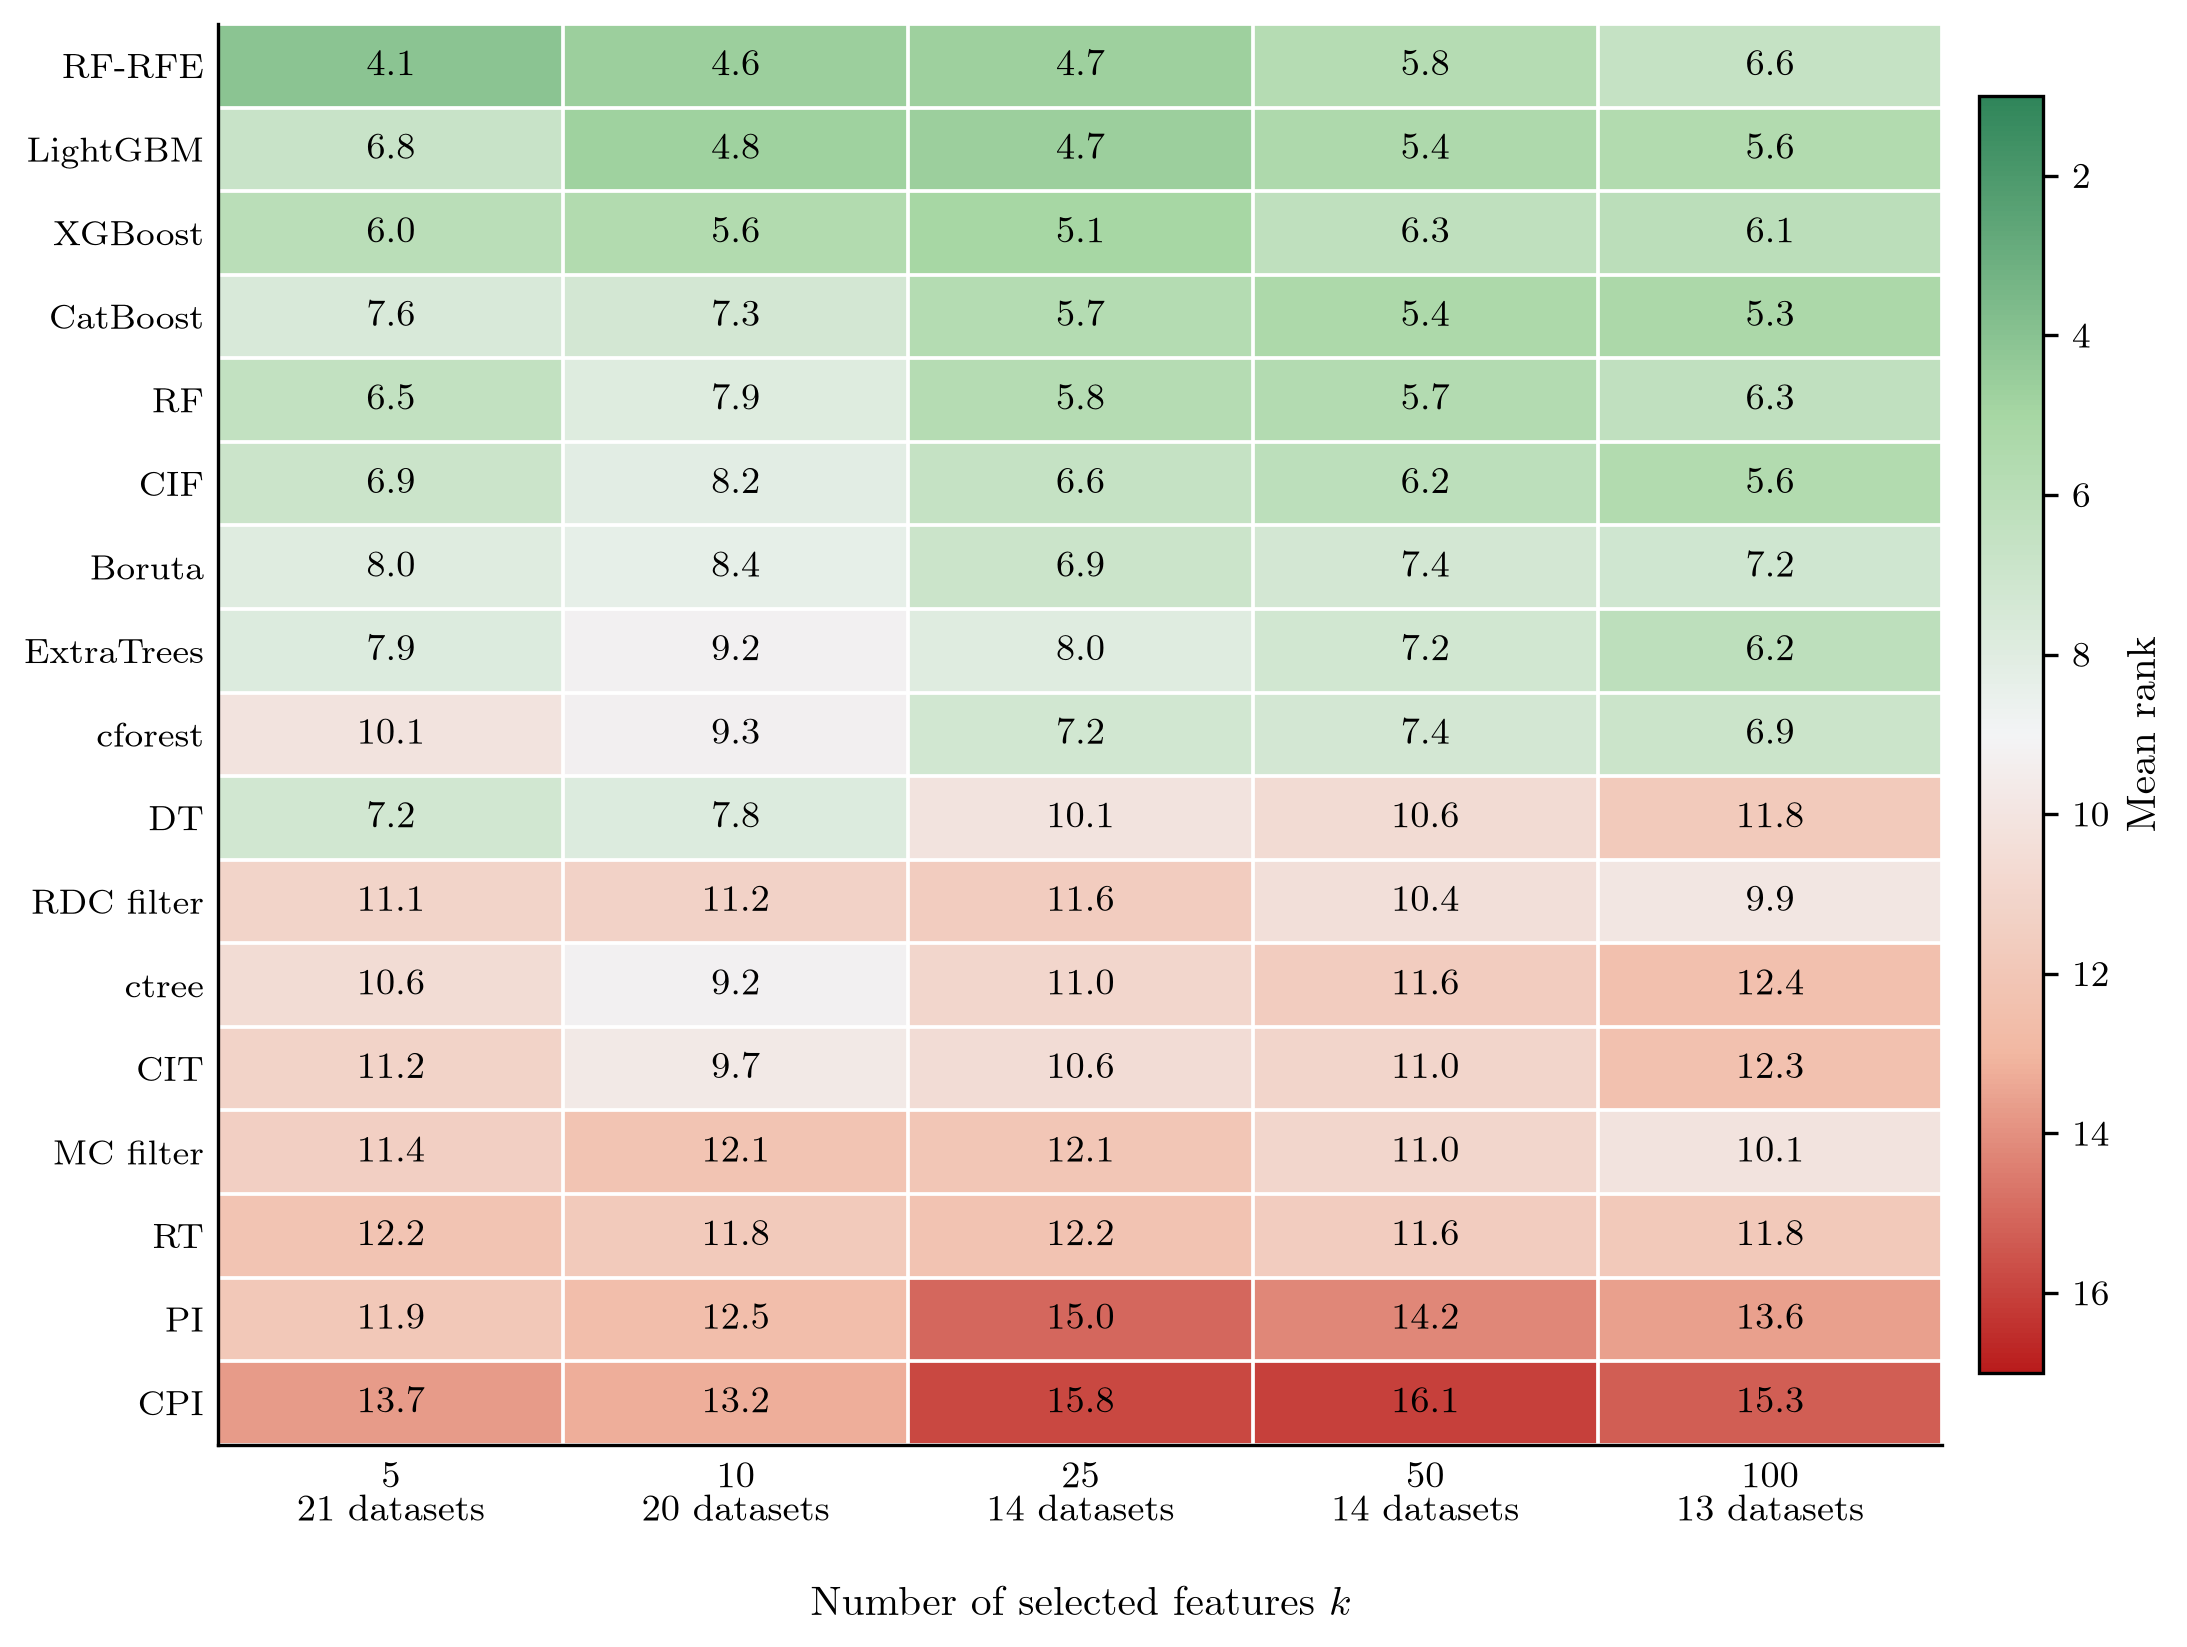
\includegraphics[width=0.86\linewidth]{figures/classification_k_trajectory.png}
  \caption{Classification mean rank by number of selected features. Rows show
  all 17 feature selection methods, averaged across downstream models at each
  value of $k$; lower ranks are better. The columns for $k=5,10,25,50,100$ use
  21, 20, 14, 14, and 13 datasets.}
  \label{fig:k-trajectory}
\end{figure}

\begin{figure}[!htbp]
  \centering
  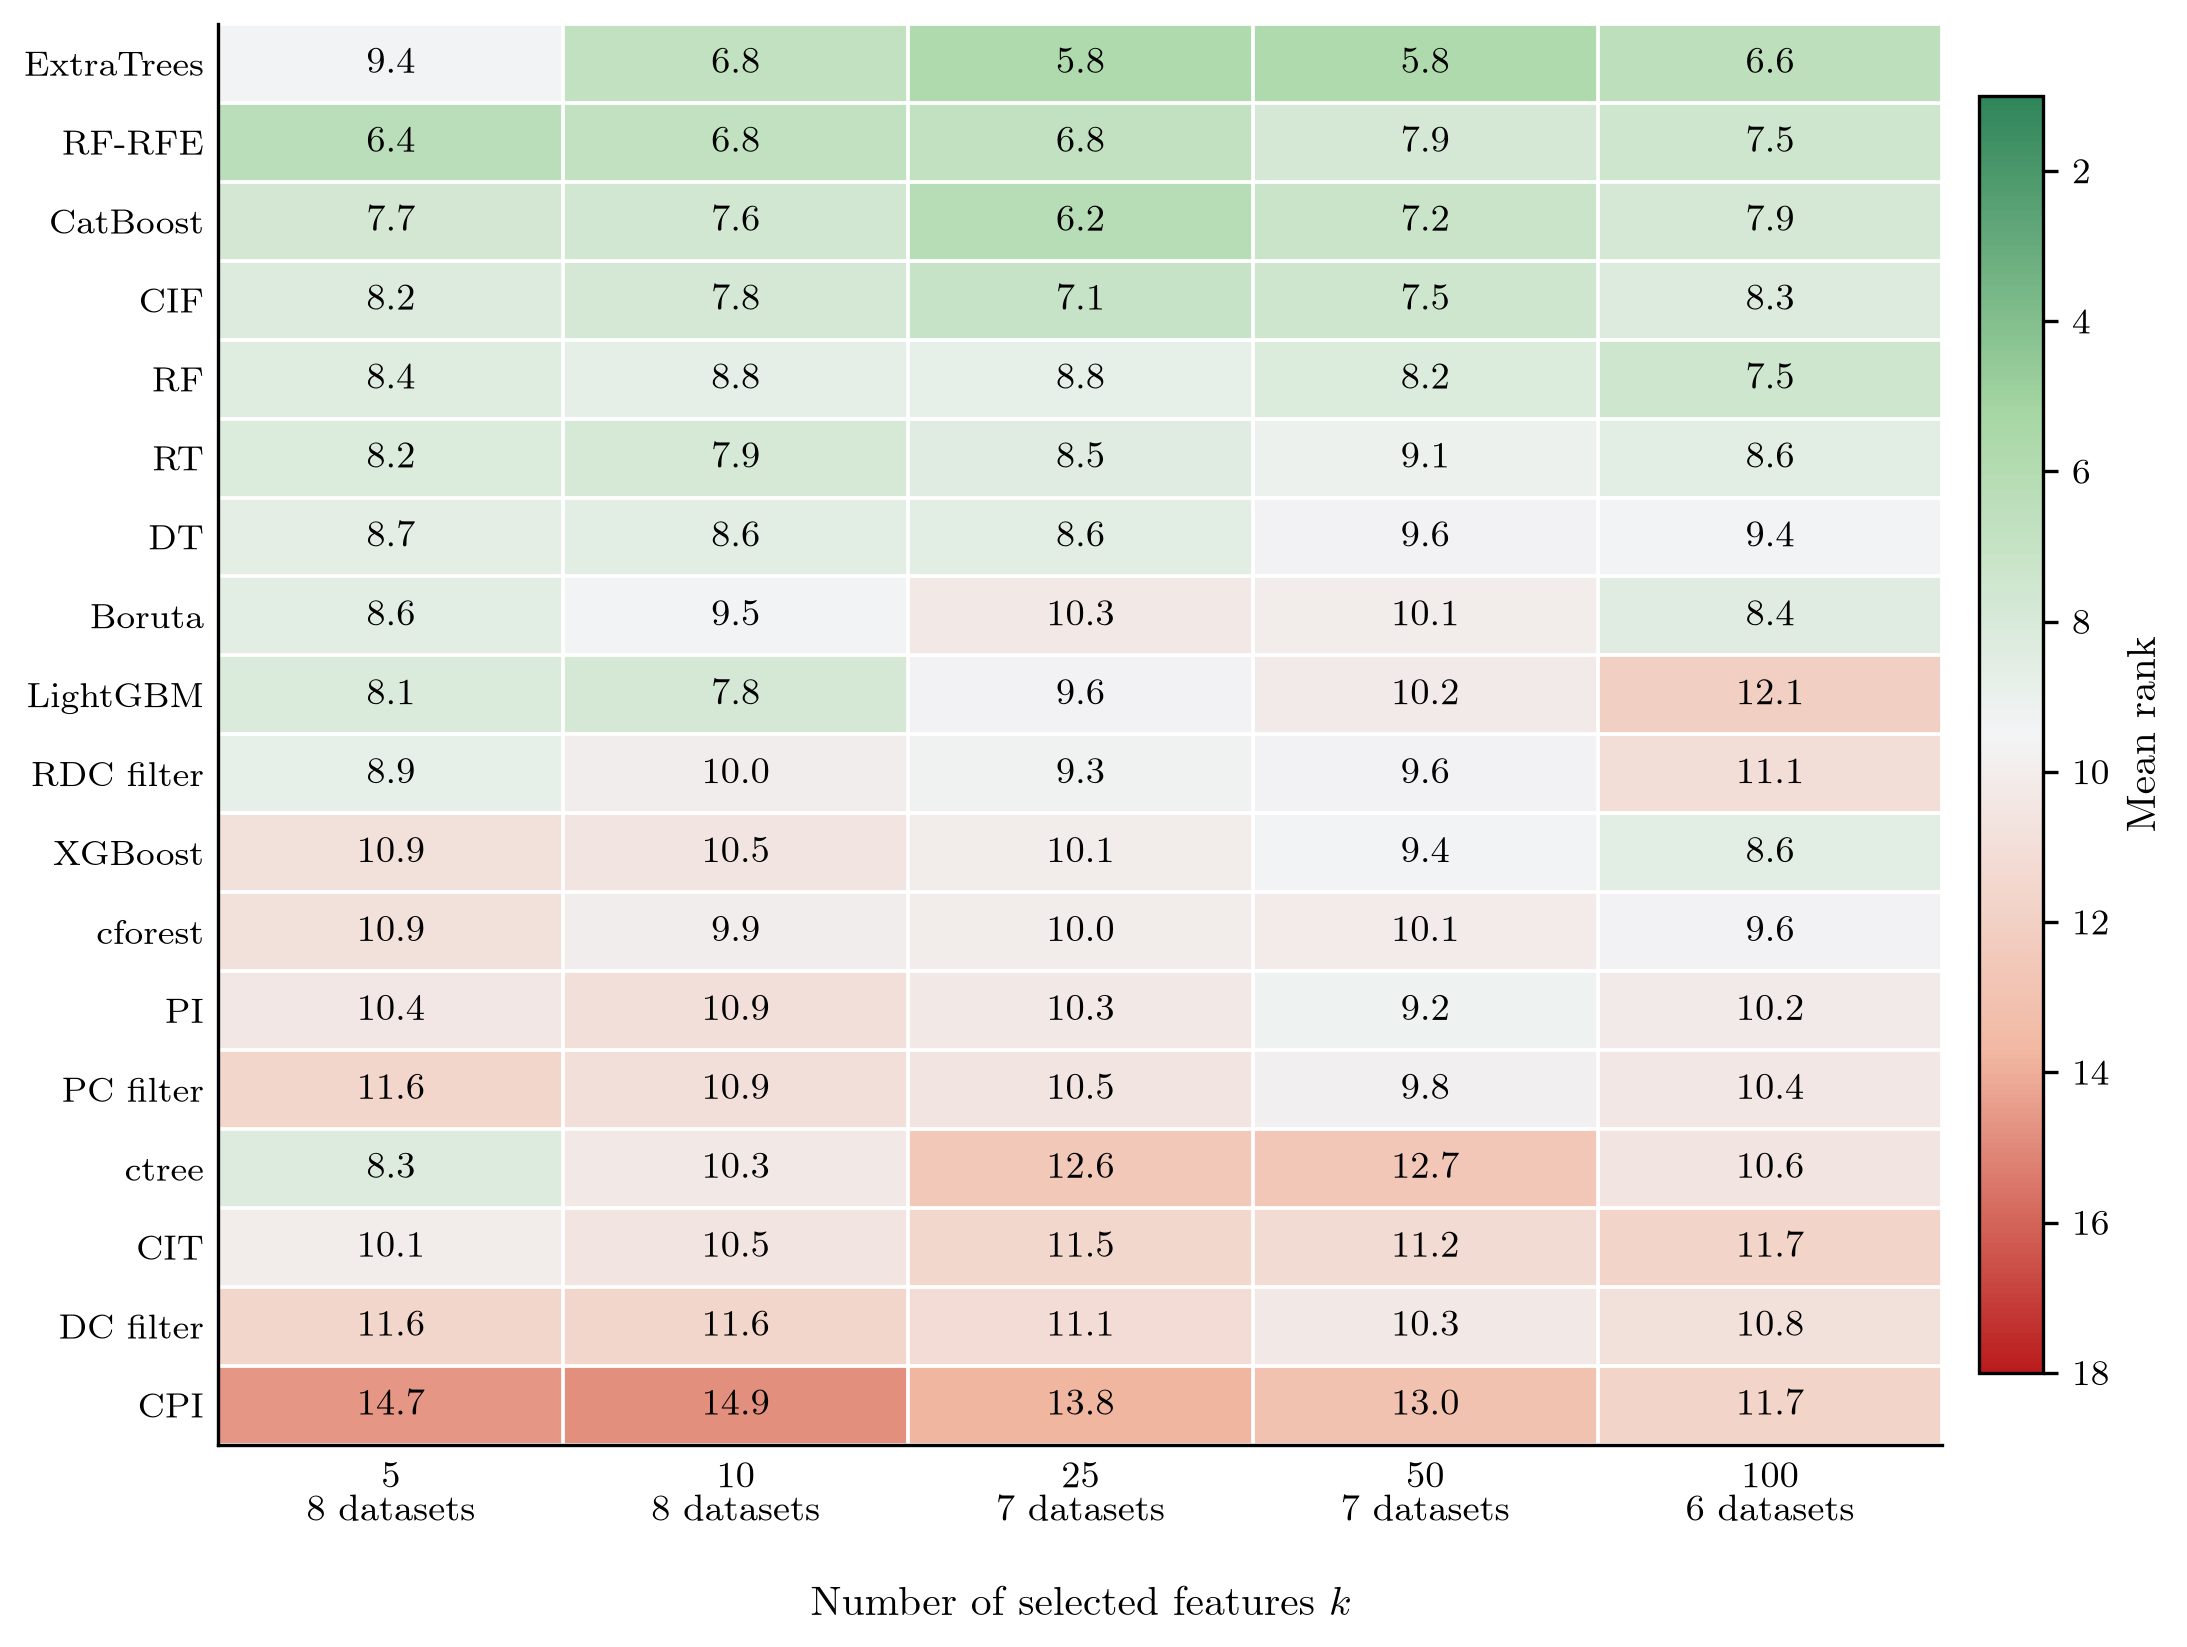
\includegraphics[width=0.86\linewidth]{figures/regression_k_trajectory.png}
  \caption{Regression mean rank by number of selected features. Rows show all
  18 feature selection methods, averaged across downstream models at each value
  of $k$; lower ranks are better. The columns for $k=5,10,25,50,100$ use 8, 8,
  7, 7, and 6 datasets.}
  \label{fig:regression-k-trajectory}
\end{figure}

\FloatBarrier

\subsection{High-dimensional datasets and small \texorpdfstring{$k$}{k}}
\label{sec:boundary}

On real data CIF ranks lowest at small $k$ and on wide datasets. At small $k$
it ranks 7th or 8th of 17 in classification on the complete-case panel
(\cref{fig:k-trajectory}). On wide datasets its scores peak before the full
feature set. Across the 15 classification datasets with more than 100
features, CIF first reaches its best score at an intermediate value of $k$
($100 < k < p$) in 29 of 45 dataset-learner combinations, and at the full
feature set ($k=p$) in 7 of 45.

\Cref{fig:high-p-boundary} shows this pattern by downstream learner. Scores
peak at intermediate $k$ on 8 of 15 LR datasets, 12 of 15 SVM datasets, and 9
of 15 KNN datasets. The full feature set helps mainly LR. Moving
from $k=100$ to $k=p$ changes the LR score by $+0.026$ on average, and LR first
reaches its best score at $k=p$ on 5 of 15 datasets. For SVM and KNN the mean
changes are $-0.053$ and $-0.071$.

In the 6 high-dimensional regression datasets, full-feature evaluation is
rarely best. Of the 18 dataset-learner combinations, 12 peak at or below
$k=100$ and 2 at $k=p$. The change from $k=100$ to $k=p$ has a mean of
$-0.270$ and a median of $-0.076$.

\begin{figure}[!htbp]
  \centering
  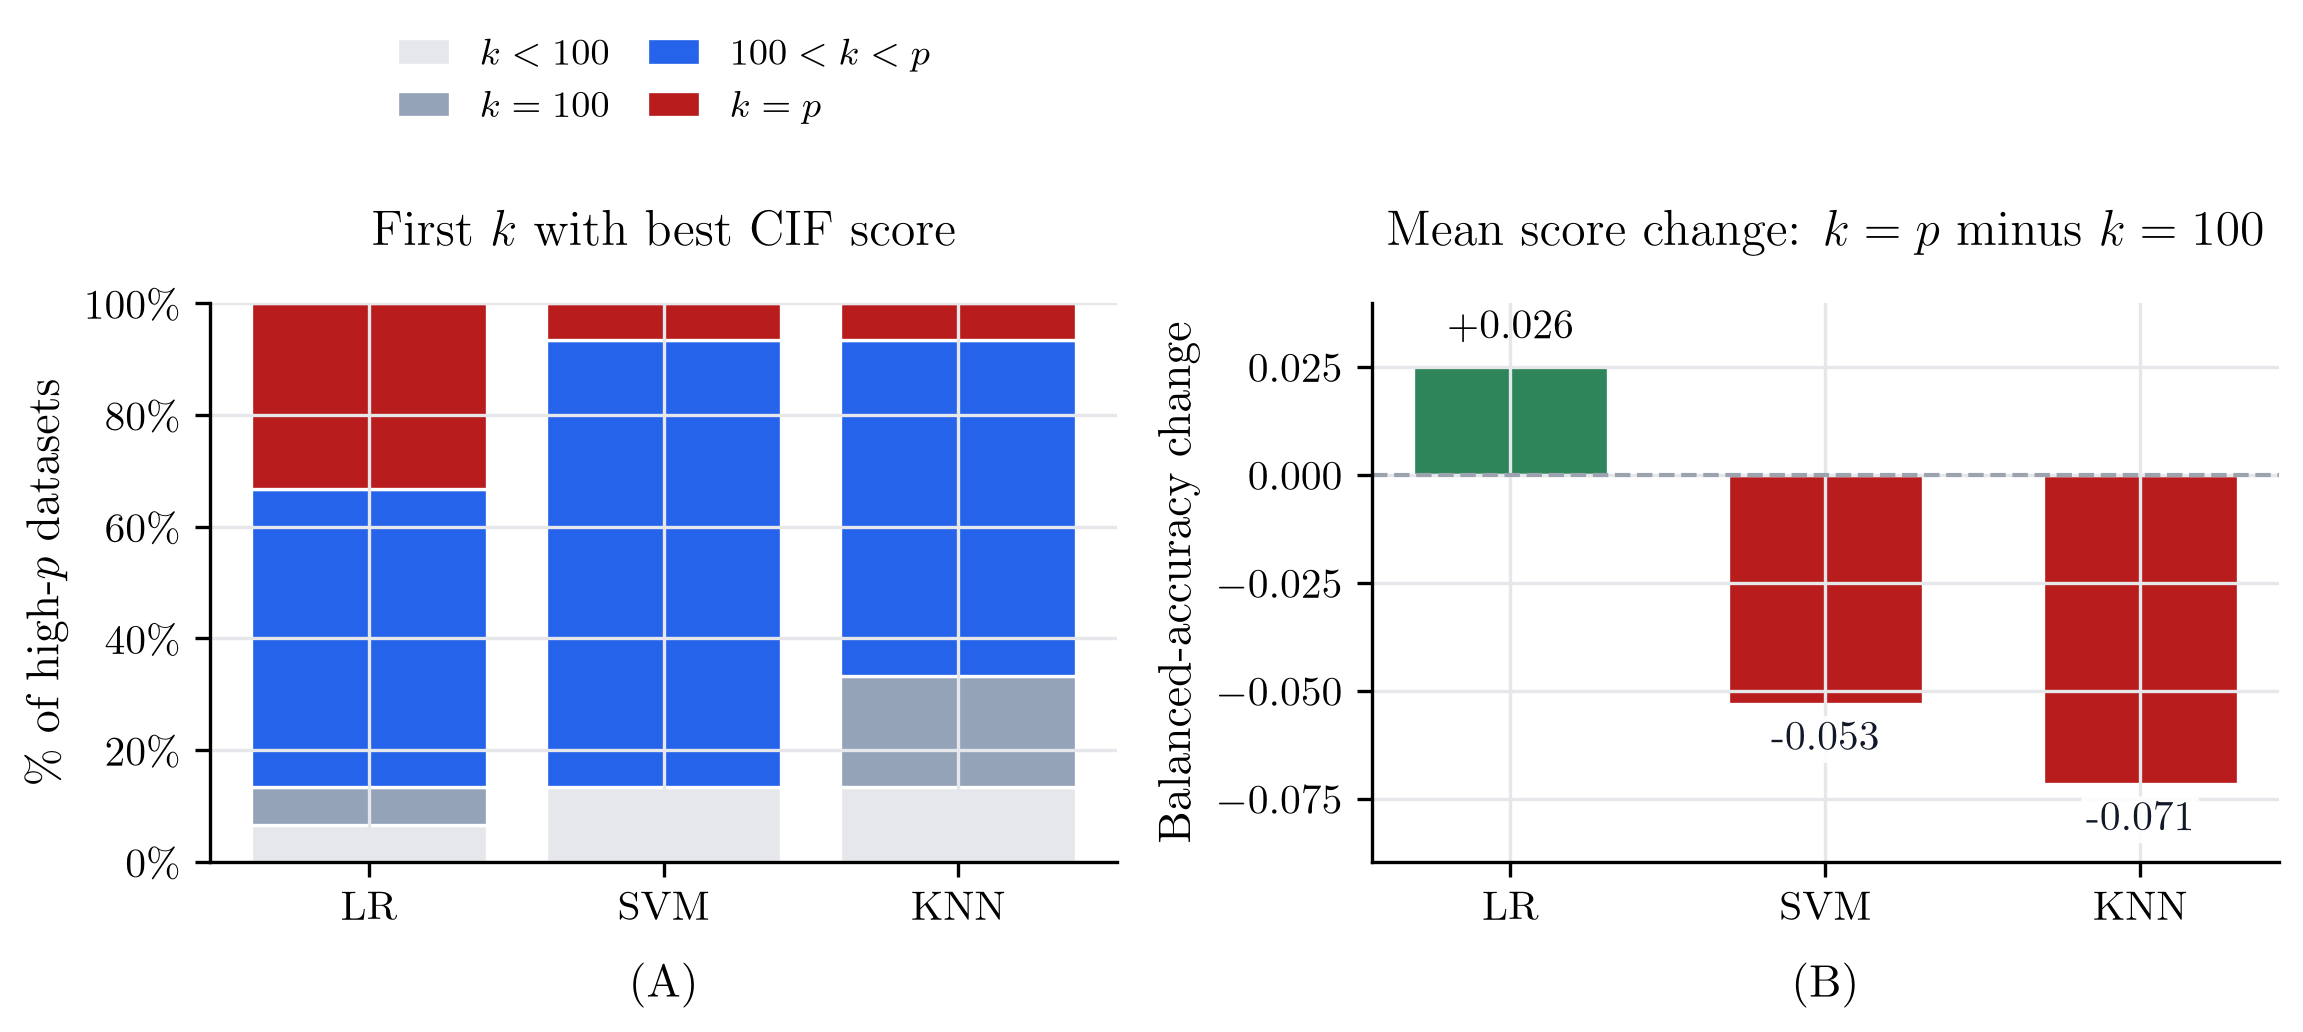
\includegraphics[width=0.84\linewidth]{figures/high_p_boundary_summary.png}
  \caption{Where CIF's classification scores peak as $k$ increases, by
  downstream learner. (A) shows, for each learner, the percentage of 15
  datasets where the first evaluated $k$ attaining the best observed CIF score
  falls below 100, at 100, between 100 and $p$, or at $k=p$. (B) shows the mean
  balanced accuracy change from $k=100$ to $k=p$.}
  \label{fig:high-p-boundary}
\end{figure}

\subsection{Synthetic recovery}
\label{sec:synthetic-recovery}

On synthetic datasets with known informative features, CIF sits at or below
the median position of the methods run on each task
(\cref{tab:synthetic-head}). It recovers true features within the top-$k$ list
more reliably than it places one first. On the redundant-feature designs,
where correlated copies of informative features count as hits, CIF ranks 1st
of 16 in regression and tied 7th of 15 in classification.
\Cref{fig:synthetic-topk-curves} shows recovery as $k$ grows.

\begin{table}[!htbp]
  \centering
  \footnotesize
  \setlength{\tabcolsep}{6pt}
  \begin{tabular}{@{}lcccc@{}}
    \toprule
    & \multicolumn{2}{c}{Classification} & \multicolumn{2}{c}{Regression} \\
    \cmidrule(lr){2-3}\cmidrule(l){4-5}
    \tablehead{Metric} & {Value} & Rank & {Value} & Rank \\
    \midrule
    Selected features that are informative & 35.3\% & \countfrac{8}{15} & 39.1\% & \countfrac{11}{16} \\
    Top-1 hit rate & 65.5\% & \countfrac{10}{15} & 84.5\% & \countfrac{10}{16} \\
    True or redundant (redundant design only) & 82.4\% & \countfrac{7.5}{15} & 83.8\% & \countfrac{1}{16} \\
    \bottomrule
  \end{tabular}
  \caption{Synthetic feature recovery for CIF. The first row averages, over
  $k = 5, 10, 25, 50$, and $100$, the percentage of selected features that are
  truly informative. The top-1 hit rate is computed at $k=1$. The final row is
  computed and ranked only on the redundant-feature design for each task and
  counts true informative plus redundant features. Ranks are among the 15
  classification and 16 regression methods with synthetic runs; fractional
  ranks indicate averaged ties.}
  \label{tab:synthetic-head}
\end{table}

\begin{figure}[!htbp]
  \centering
  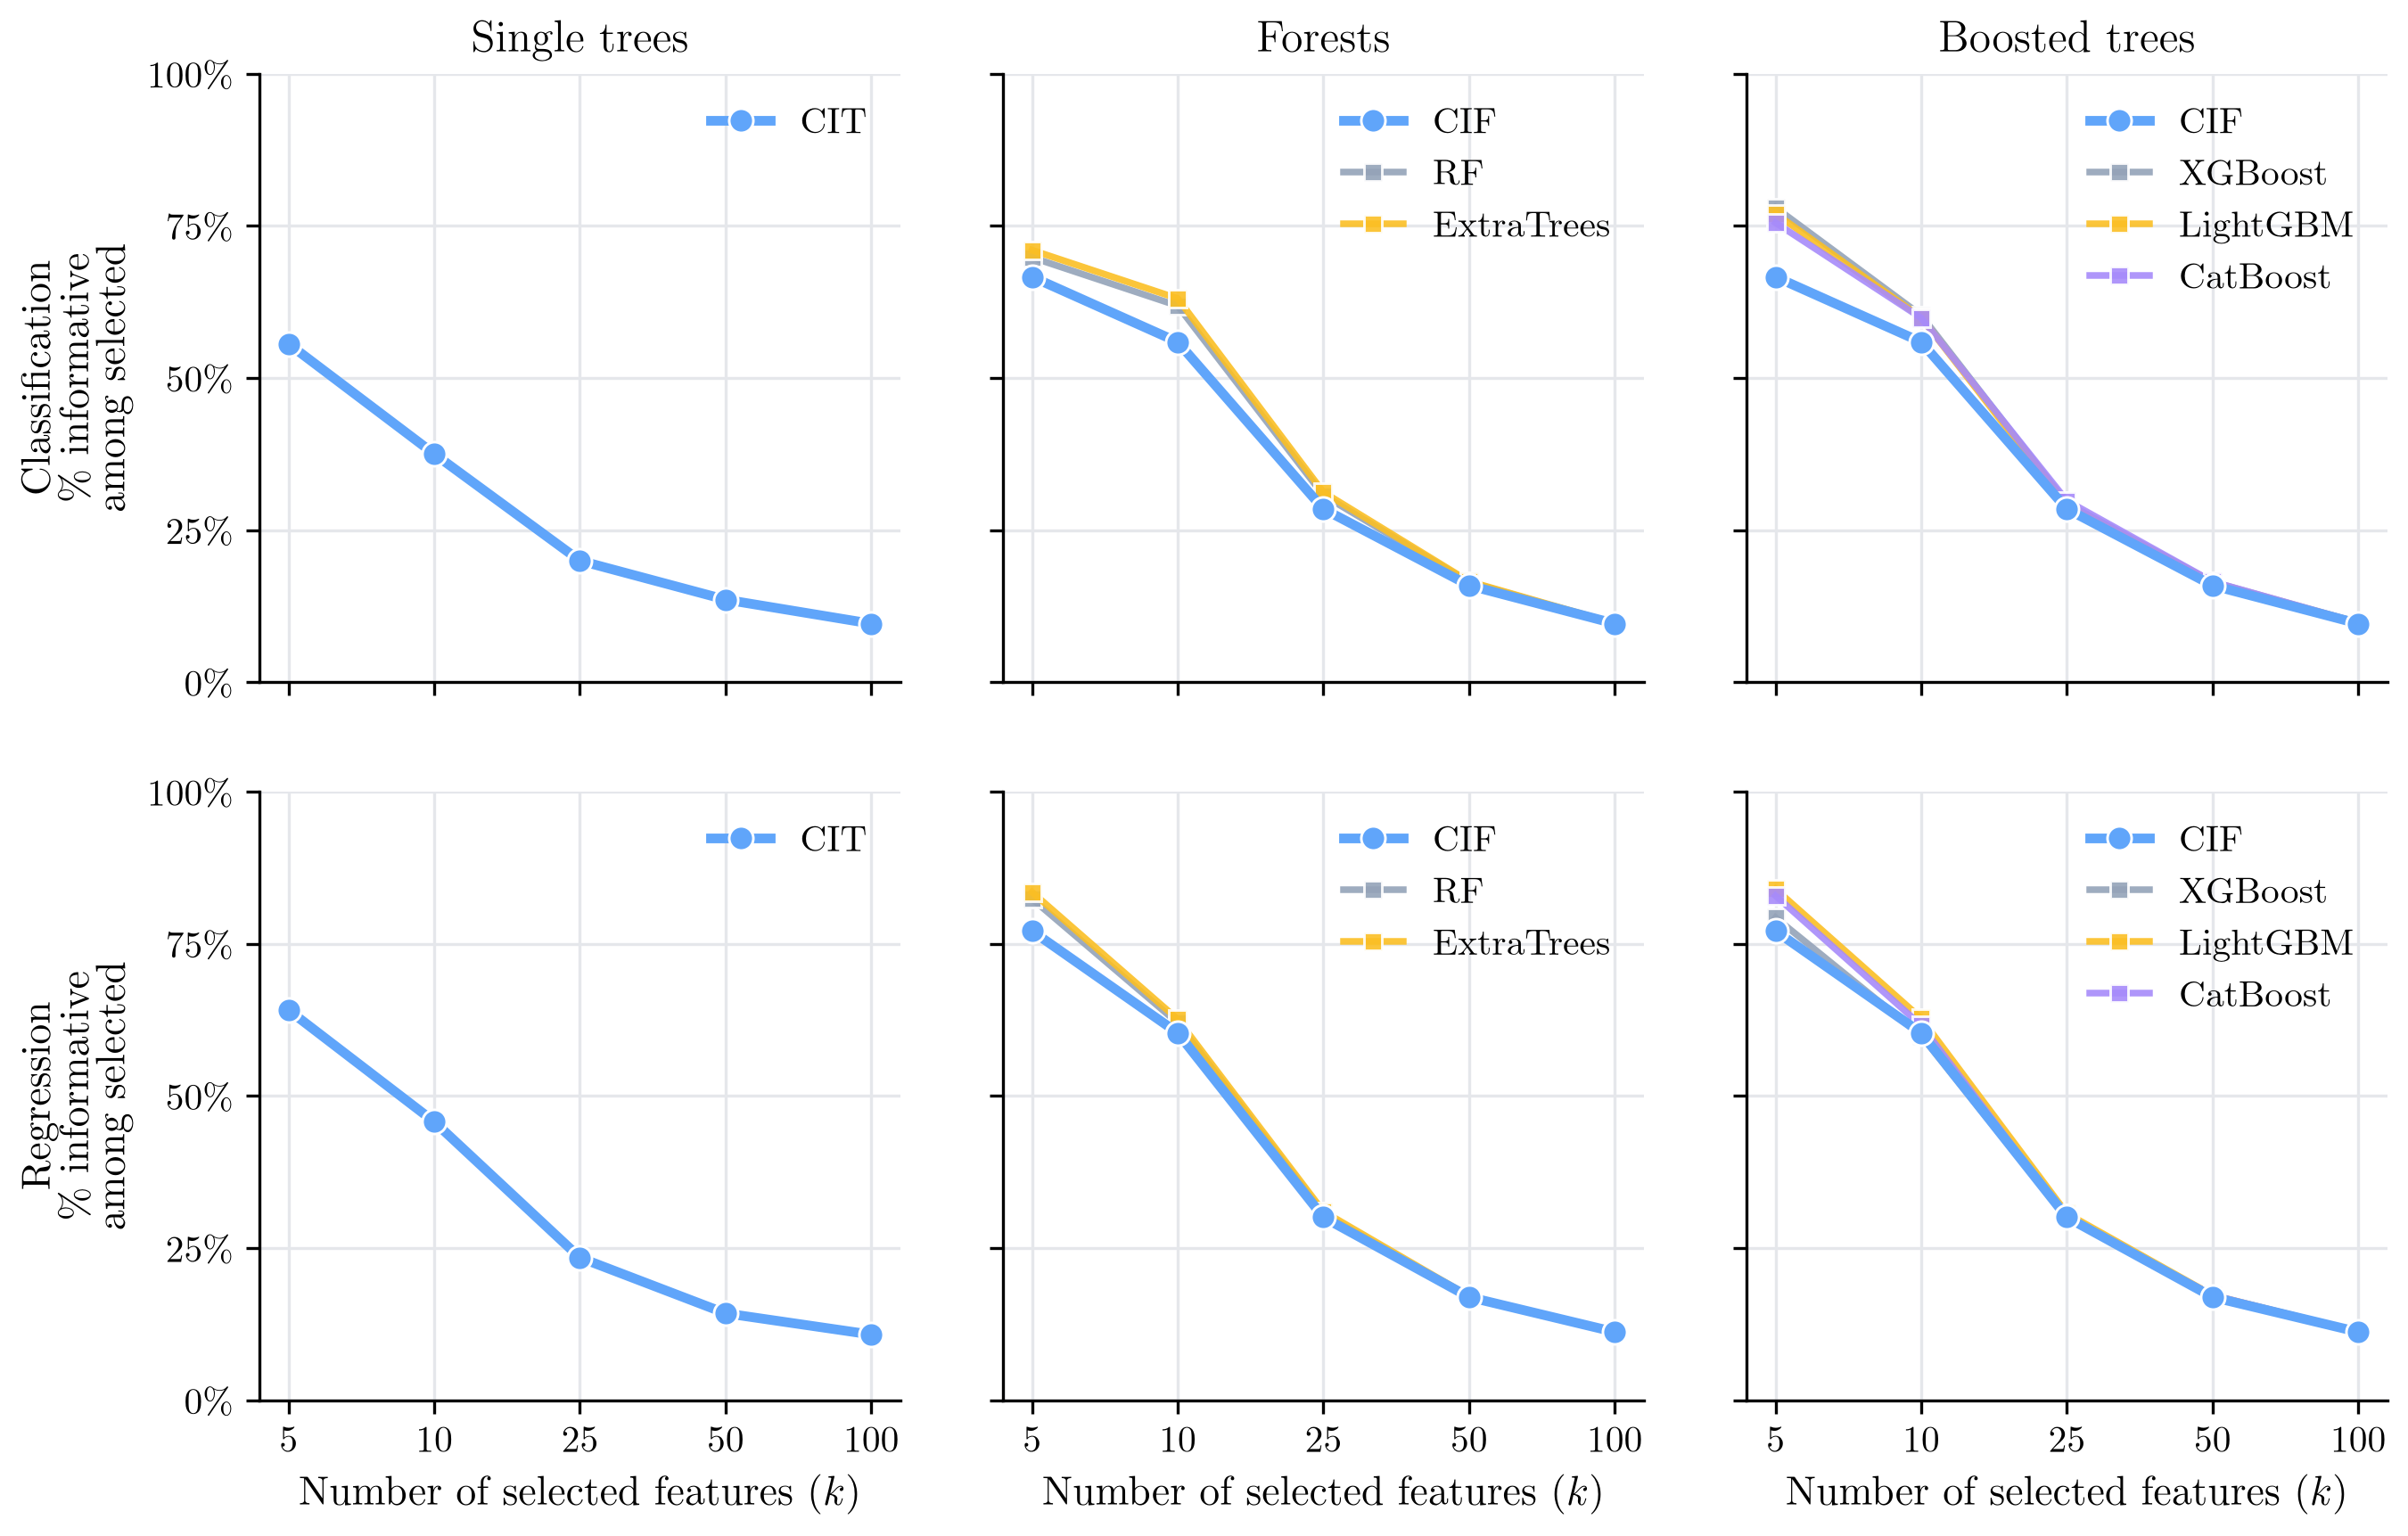
\includegraphics[width=0.84\linewidth]{figures/synthetic_topk_focus_curves.png}
  \caption{Synthetic top-$k$ recovery curves. Columns compare single trees,
  forests, and boosted trees; rows show classification and regression. Each
  value is the percentage of selected features that are truly informative.}
  \label{fig:synthetic-topk-curves}
\end{figure}

\subsection{What the CIF ranking rests on}
\label{sec:mechanism}

Of four targeted changes to the selected CIF configuration, only reducing the
forest to one tree lowers the score on every dataset, in both tasks
(\cref{tab:cif-ranking-ablation}). Split-count ranking, disabling bootstrap
sampling, and disabling feature muting change balanced accuracy by at most
0.001 on average, with intervals that include zero. In regression these three
changes lower the mean $R^2$, two of them with intervals that exclude zero, but
the three \nolinkurl{coepra} datasets set those means, and the medians stay
within 0.007 of zero.

\begin{table}[htb]
  \centering
  \footnotesize
  \setlength{\tabcolsep}{4pt}
  \renewcommand{\arraystretch}{1.08}
  \begin{tabular}{@{}llS[table-format=+1.3]S[table-format=+1.3]cc@{}}
    \toprule
    \tablehead{Task} & \tablehead{CIF change} & {Mean difference} & {Median difference} & 95\% interval & Wins--losses \\
    \midrule
    Classification & Split-count ranking & -0.001 & 0.000 & [$-$0.005, +0.002] & \winloss{12}{9} \\
    Classification & Disable bootstrap & -0.001 & 0.000 & [$-$0.004, +0.003] & \winloss{9}{12} \\
    Classification & Disable feature muting & +0.001 & 0.000 & [$-$0.001, +0.002] & \winloss{13}{5} \\
    Classification & Use one tree & -0.071 & -0.043 & [$-$0.101, $-$0.045] & \winloss{0}{22} \\
    \addlinespace
    Regression & Split-count ranking & -0.053 & -0.003 & [$-$0.142, $-$0.002] & \winloss{2}{6} \\
    Regression & Disable bootstrap & -0.064 & -0.007 & [$-$0.128, $-$0.010] & \winloss{4}{4} \\
    Regression & Disable feature muting & -0.157 & 0.000 & [$-$0.468, +0.001] & \winloss{4}{4} \\
    Regression & Use one tree & -0.658 & -0.059 & [$-$1.692, $-$0.054] & \winloss{0}{8} \\
    \bottomrule
  \end{tabular}
  \caption{CIF ablations on the real-data benchmark, 22 classification and 8
  regression datasets. Differences are the changed variant minus the selected
  CIF configuration in balanced accuracy or $R^2$, paired within seed and fold
  and averaged within each dataset over downstream learners, supported standard
  values of $k$, and the 25 paired replicates; positive values favor the
  variant. Intervals are percentile bootstrap intervals for the mean over
  datasets (20{,}000 replicates); wins and losses count datasets, with exact
  ties omitted.}
  \label{tab:cif-ranking-ablation}
\end{table}

\paragraph{Support.}
The support of a ranker is the set of features that win at least one split.
Features outside it receive zero importance and follow in the tie order of
\cref{sec:rank-construction}, so a ranking carries information only within its
support. On the synthetic datasets, random forests give every feature nonzero
importance on 15 of the 16 designs, and 800 of 1,000 on the 1,000-feature
classification design. On 13 of the 16 designs, CIF's support keeps 90 to
100\% of the planted features, so the support serves as a shortlist. A single
CIT splits on few features, so zero-importance filler makes up most of its
top-$k$ list: 52, 81, and 90\% of its top 10, 25, and 50 features, against 0,
3, and 14\% for CIF and none for random forests. This is consistent with CIT
ranking near the bottom of the benchmark.

\paragraph{Feature use in sampled forests.}
In sparse designs, feature sampling keeps informative features out of most CIF
splits (\cref{app:candidate-availability}). CIT, which considers every feature
at each node, uses informative features in 100.0\% of classification splits
and 93.5\% of regression splits. Over the 12 classification forest designs,
CIF uses them in 33.2\% of splits, against 91.7\% for CIF-all, 8.4\% for RF,
and 6.5\% for ExtraTrees. RF and ExtraTrees grow to purity, so most of their
splits are deep splits on noise, while CIF stops at the permutation test. With
32 of 1,000 features sampled at a node and two informative, an informative
feature is a candidate at 6.3\% of nodes, and when the sampled subset holds
none, Stage~A selects from the noise it was given.

\subsection{Runtime ablations}
\label{sec:results-practical}

\Cref{tab:runtime-ablations} changes one setting at a time and reports fitting
time relative to the selected configuration of the same estimator. Each ratio
is the median over datasets of the per-dataset ratio, given as the range over
the four task groups (classification and regression, real and synthetic).
Ratios above 1 are slower. \Cref{app:complexity-details} links each row to the
work terms it affects.

\begin{table}[!htbp]
  \centering
  \footnotesize
  \setlength{\tabcolsep}{4pt}
  \begin{tabular}{@{}lccccc@{}}
    \toprule
     & \multicolumn{2}{c}{CIT} & \multicolumn{3}{c}{CIF} \\
    \cmidrule(lr){2-3}\cmidrule(l){4-6}
    \tablehead{Change} & Time ratio & \shortstack{Top-10 F1\\change} & Time ratio & \shortstack{Downstream\\change} & \shortstack{Recovery\\change} \\
    \midrule
    Disable adaptive stopping & 0.88 to 0.99 & 0 & 0.96 to 1.00 & 0 & 0 \\
    Auto budget, adaptive stopping & 1.18 to 1.56 & $\le 0.016$ & 1.30 to 2.0 & & $\le 0.030$ \\
    Auto budget, no stopping & 3.8 to 8.2 & $\le 0.016$ & 5.8 to 15 & & $\le 0.025$ \\
    Disable threshold scanning & 2.7 to 34 & $\le 0.033$ & 7.9 to 30 & $\le 0.003$ & $\le 0.010$ \\
    Disable feature scanning & 0.81 to 3.0 & $\le 0.058$ & 1.0 to 5.2 & $\le 0.003$ & $\le 0.008$ \\
    Exact threshold search & 0.91 to 1.10 & $\le 0.004$ & 1.3 to 19 & $\le 0.009$ & $\le 0.018$ \\
    Histogram with 32 bins & & & 0.05 to 0.14 & $\le 0.008$ & $\le 0.013$ \\
    Disable feature muting & 0.97 to 0.98 & 0 & 0.91 to 1.00 & $\le 0.001$ & $\le 0.003$ \\
    Disable bootstrap sampling & & & 0.94 to 1.69 & $\le 0.012$ & $\le 0.011$ \\
    Max-type Stage~B rule & & & 0.14 to 0.61 & $\le 0.005$ & $\le 0.007$ \\
    Remove both corrections & 0.52 to 1.8 & $\le 0.063$ & 0.03 to 0.34 & $\le 0.004$ & $\le 0.011$ \\
    \bottomrule
  \end{tabular}
  \caption{Runtime ablations of CIT and CIF on the runtime panel of 23 datasets
  (15 classification and 8 regression; 9 real and 14 synthetic), five seeds per
  dataset. Time ratios are medians over datasets of the per-dataset ratio to
  the selected configuration, given as the range over the four task groups.
  Top-10 F1 is the harmonic mean of precision and recall of the ten
  highest-ranked features against the planted informative set. Score columns
  give the largest absolute change across task groups in mean top-10 F1 for
  CIT, and in the dataset-mean downstream score and synthetic feature recovery
  for CIF; bounds are rounded upward to 0.001. The auto-budget runs record
  recovery but no downstream score. Empty cells are settings that do not apply
  to, or were not ablated for, that estimator. Every time is the second of two
  identical fits, so compilation is excluded.}
  \label{tab:runtime-ablations}
\end{table}

At the benchmark's minimum budget, adaptive stopping is inert by construction
(\cref{sec:theory-adaptive}). Switching it off leaves every tree unchanged, and
the time ratios near 1 measure only the cost of the check. The result does not
depend on how forest trees are scheduled, since a forest with one worker and
the full thread pool inside each tree gives 0.95 to 1.01.

At the auto budget, where the rule can act, adaptive stopping brings the tree
to 0.14 to 0.37 and the forest to 0.11 to 0.25 of their no-stopping time, with
recovery changes of at most 0.030.

Of the runtime controls, the threshold scan has the largest effect. Testing
candidate thresholds in order of weighted child impurity and stopping at the
first rejection makes trees 2.7 to 34 times and forests 7.9 to 30 times faster
than testing every candidate. The candidate count has the next largest effect.
For the forest, exact threshold search is 1.3 to 19 times slower than the
256-bin histogram, and a 32-bin histogram is 7 to 21 times faster, with
downstream changes of at most 0.009. Feature scanning matters most on the real regression datasets. The
max-type rule fits the forest in 0.14 to 0.61 of the reference time.

Removing the two corrections changes the statistical rule as well as the
fitting time. It deepens trees from a mean of 6.5 and 7.2 levels to 10.7 and
13.4, and moves top-10 recovery by up to 0.063. The selected configuration
keeps both corrections.

The pattern holds on the 14 Benchmark-size datasets, with up to 20,000
observations and 5,000 features. Switching adaptive stopping off changes tree
time by 0.80 to 1.01 (medians 0.97 in classification and 0.88 in regression)
and forest time by 0.99 to 1.34 (medians 1.00 and 1.03). Threshold scanning
saves a median 17 times in classification and 45 times on spam, and removing
the corrections runs in 0.01 to 1.26 of the reference time. The slowest single
tree is gisette at 29 minutes, where the feature correction over 5,000 features
sets a large minimum budget for each feature test.

\subsection{Stage~B construction comparison}
\label{sec:results-stageB}

This section compares the per-threshold and max-type Stage~B rules on size,
power, threshold placement, cost, and the benchmark rankings. Both rules
control the false-split rate. At matched realized size the max-type rule has
slightly lower power, and it places the threshold slightly less precisely. It
is cheaper once a node has many candidates.

The complete-node false-split rate is below 0.05 for both rules in all 36
design cells (\cref{tab:stageB-calibration}, \cref{app:stageB-tables}). These
rates include the Stage~A test over five predictors, so they bound the
threshold test from below rather than measure it.

The Stage-B-only study measures the threshold test itself
(\cref{tab:stageB-only}). At nominal level 0.05 the per-threshold rule has size
0.000 to 0.027, with means 0.018, 0.011, and 0.006 at 16, 64, and 256 bins.
The max-type rule has size 0.023 to 0.044, with means 0.033, 0.035, and 0.035.
Every 95\% Clopper-Pearson upper limit is below 0.056. Both rules are valid at
a fixed node for a predictor fixed without the response. The reverse
cardinality bias of \cref{sec:rank-construction} appears as a threefold fall in
per-threshold size across bin settings, while the max-type size does not move.

\begin{table}[!htbp]
  \centering
  \footnotesize
  \setlength{\tabcolsep}{4pt}
  \begin{tabular}{@{}lrrrrrrrrr@{}}
    \toprule
     & & & \multicolumn{4}{c}{Size at nominal 0.05} & & \multicolumn{2}{c}{Size-matched power} \\
     & & & \multicolumn{2}{c}{Per-threshold} & \multicolumn{2}{c}{Max-type} & Match & & \\
    \tablehead{Task} & $n$ & Bins & Adaptive & None & Adaptive & None & size & Per-threshold & Max-type \\
    \midrule
    Classification & 100 & 16 & 0.013 & 0.013 & 0.032 & 0.033 & 0.050 & 0.390 & 0.379 \\
     & 100 & 64 & 0.007 & 0.007 & 0.036 & 0.039 & 0.044 & 0.385 & 0.354 \\
     & 100 & 256 & 0.007 & 0.007 & 0.036 & 0.042 & 0.034 & 0.335 & 0.318 \\
     & 200 & 16 & 0.010 & 0.011 & 0.037 & 0.039 & 0.050 & 0.643 & 0.618 \\
     & 200 & 64 & 0.008 & 0.009 & 0.035 & 0.039 & 0.050 & 0.630 & 0.615 \\
     & 200 & 256 & 0.003 & 0.003 & 0.039 & 0.039 & 0.031 & 0.562 & 0.538 \\
     & 500 & 16 & 0.015 & 0.015 & 0.032 & 0.037 & 0.050 & 0.958 & 0.953 \\
     & 500 & 64 & 0.007 & 0.007 & 0.029 & 0.035 & 0.050 & 0.961 & 0.964 \\
     & 500 & 256 & 0.000 & 0.001 & 0.023 & 0.032 & 0.034 & 0.958 & 0.952 \\
    Regression & 100 & 16 & 0.019 & 0.019 & 0.023 & 0.031 & 0.050 & 0.292 & 0.281 \\
     & 100 & 64 & 0.013 & 0.013 & 0.029 & 0.035 & 0.050 & 0.305 & 0.285 \\
     & 100 & 256 & 0.011 & 0.010 & 0.031 & 0.037 & 0.050 & 0.317 & 0.299 \\
     & 200 & 16 & 0.027 & 0.026 & 0.033 & 0.038 & 0.050 & 0.591 & 0.581 \\
     & 200 & 64 & 0.017 & 0.017 & 0.033 & 0.043 & 0.050 & 0.619 & 0.598 \\
     & 200 & 256 & 0.008 & 0.009 & 0.041 & 0.044 & 0.050 & 0.632 & 0.579 \\
     & 500 & 16 & 0.026 & 0.026 & 0.031 & 0.032 & 0.050 & 0.947 & 0.942 \\
     & 500 & 64 & 0.015 & 0.016 & 0.029 & 0.033 & 0.050 & 0.966 & 0.952 \\
     & 500 & 256 & 0.005 & 0.006 & 0.026 & 0.034 & 0.046 & 0.963 & 0.951 \\
    \bottomrule
  \end{tabular}
  \caption{Stage-B-only study: the threshold test in isolation, with one
  Gaussian predictor fixed without the response and the Stage~A test disabled.
  Size is the false-split rate of a depth-one tree at nominal level 0.05 over
  1,500 null replicates per cell (three seeds of 500) under adaptive stopping
  and no stopping (None); every 95\% Clopper-Pearson upper limit is below
  0.056. Size-matched power, shown for adaptive stopping at the middle effect
  ($\delta = 0.10$ in classification, $0.4$ in regression), is interpolated
  against realized size over the nominal grid from 0.02 to 0.50 (600 replicates
  per cell and level) to the match size: 0.05, or the largest realized size
  both rules reach where the per-threshold rule does not reach 0.05.}
  \label{tab:stageB-only}
\end{table}

Matched at the same realized size, the max-type minus per-threshold difference
in power ranges from $-0.054$ to $+0.034$ over the 108 cell and effect
combinations. The max-type rule is lower in 67 and higher in 25. The mean
difference is $-0.006$, with a 95\% bootstrap interval of $-0.011$ to $-0.002$
that resamples the 18 cells, and $-0.005$ ($-0.009$ to $-0.002$) over the 13
cells matched at size 0.05. It has no trend in the bin setting. In the other
five cells the per-threshold rule does not reach size 0.05 even at nominal
0.50, and the match is at the largest size both rules reach.

Two reruns bound the Monte Carlo error. With larger replicate counts at a
fourth seed, the mean difference is $-0.006$ ($-0.008$ to $-0.003$); a
parametric bootstrap of the whole matching procedure puts a standard error of
about 0.017 on each difference, so the smallest detectable difference is about
0.03. With the planted step moved to the 85th percentile, the mean difference
is $-0.004$ ($-0.008$ to $0.000$), with a standard error of about 0.038 and a
detectable difference of about 0.08. The Stage-B-only sizes stay in the ranges
above.

At a common nominal level of 0.05, the max-type rule splits more often, by 0.03
on average and up to 0.12 in the complete-node design (\cref{tab:stageB-power})
and by 0.10 in the Stage-B-only study. The gap grows with the candidate count,
0.015 at 16 bins, 0.029 at 64, and 0.049 at 256, because the per-threshold
power falls as the threshold correction tightens. The gap therefore reflects
the lower realized size of the per-threshold rule, which the matched
comparison above removes.

The max-type rule places the threshold less precisely. On each rule's own
detections, the max-type threshold sits a median 0.19 standard deviations from the planted cut
against 0.15 for the per-threshold rule, and 87\% of its detections fall on
the planted predictor against 90\%.

\Cref{tab:stageB-scaling} reports the cost of the two rules. With no stopping and
256 bins, one classification tree under the per-threshold rule takes 3.5, 14,
and 59 seconds at $n=1{,}000$, $4{,}000$, and $16{,}000$ (0.8, 8.8, and 54 in
regression); the max-type rule takes 0.3, 1.4, and 6.3 seconds. The ratio grows
with the bin setting as the $K^2/\alpha$ against $BK$ accounting predicts. At
16 bins the max-type rule is 1.1 to 1.3 times slower, because its 999
permutations exceed the 340 the per-threshold rule needs for 17 candidates. At
64 bins it is 1.5 to 2.1 times faster, and at 256 bins 2.8 to 13 times.
Adaptive stopping shortens the per-threshold test by 1.2 to 1.6, 2.2 to 3.2,
and 3.8 to 7.8 times at the three bin settings, so with adaptive stopping the
max-type advantage is 1.0 to 1.3, 1.4 to 2.1, and 2.2 to 7.7. Held at 999
permutations per candidate instead, the per-threshold rule never splits at 64
or 256 bins, because $\alpha/K$ falls below the resolution $1/(B+1)$. Fitted
depths barely differ: 5.0 to 10.7 levels for the max-type rule against 4.0 to
10.0.

On the six Stage~B real datasets (\cref{tab:stageB-real}), the max-type rule
scores higher in 8 of the 12 dataset and stopping-mode cells and equal in one.
It is higher by 0.016 and 0.026 balanced accuracy on vowel, 0.049 and 0.026
$R^2$ on facebook, 0.060 and 0.033 on imports-85, and 0.008 and 0.005 on
residential. It is lower by 0.018 and 0.020 on page-blocks, and on spam lower
by 0.006 with adaptive stopping and equal with no stopping. Its fitting time is
1.2 to 2.4 times shorter with adaptive stopping and 1.0 to 8.3 times shorter
with no stopping on the four datasets whose nodes admit many candidates. It is
16\% and 10\% slower on residential. Fitted depths agree within about one
level (5.4 to 11.4 for the per-threshold rule, 4.8 to 12.4 for the max-type
rule). The Spearman agreement of the two rules' feature importances is 0.36 to
0.88, so the max-type rule produces a different ranking rather than the same
ranking at lower cost.

In the head-to-head forest timing, the max-type rule is 10 to 27 times faster
than the per-threshold rule on the synthetic cells at $n\le 8{,}000$ and 21 to
36 times faster at $n=32{,}000$ (13 to 36 times on the cells that
\citet{MilletichDownesHirst2026citrees} tabulate). The runtime panel of
\cref{tab:runtime-ablations} shows smaller ratios, 1.6 to 7 times, because its
nodes admit fewer candidates. On the ten real datasets the max-type rule
reduces madelon from 21 to 2.6 seconds, gamma from 44 to 21, and isolet from 18
to 9.1, and changes the other seven by at most 1.6 seconds.

The max-type extension shows what the rule does to the rankings
(\cref{tab:maxt-benchmark-rankings}). Of its 1,880 possible ranking runs, 88
were not run because their per-threshold counterpart had not completed, and
1,785 of the remaining 1,792 completed. The seven that did not are CIF with the
RDC selector and honesty off on isolet, gisette, and letter, the same cells
excluded from the per-threshold benchmark (\cref{app:methods}). Ranked on the
all-method panels, the max-type forest moves from 3.5 to 5 of 17 in
classification and from 2 to 4 of 18 in regression, and the max-type tree
keeps its position in both tasks. The per-threshold rule is the higher of the
two on 59 to 63\% of datasets. The case for the max-type rule therefore rests
on cost and calibration rather than on the rankings.

\begin{table}[!htbp]
  \centering
  \footnotesize
  \setlength{\tabcolsep}{5pt}
  \begin{tabular}{@{}llrrrrrr@{}}
    \toprule
     & & \multicolumn{2}{c}{Per-threshold} & \multicolumn{2}{c}{Max-type} & \multicolumn{2}{c}{Paired difference} \\
    \tablehead{Task} & Method & Mean rank & Position & Mean rank & Position & Score & Datasets \\
    \midrule
    Classification & CIF & 5.86 & 3.5 & 6.31 & 5 & $-0.0014$ & 22 \\
     & CIT & 13.14 & 16 & 13.00 & 16 & $-0.0022$ & 23 \\
    Regression & CIF & 6.25 & 2 & 7.50 & 4 & $-0.0001$ & 8 \\
     & CIT & 11.13 & 14 & 10.88 & 14 & $-0.0085$ & 8 \\
    \bottomrule
  \end{tabular}
  \caption{Benchmark rankings under the two Stage~B rules. Mean rank and
  position are among the 17 classification and 18 regression methods on the
  all-method panels of 21 and 8 datasets, with the max-type family standing in
  for its per-threshold counterpart; the per-threshold columns repeat
  \cref{tab:method-main-comparison}. The paired difference is the max-type
  score minus the per-threshold score (balanced accuracy in classification,
  $R^2$ in regression), averaged over the datasets, downstream learners, and
  standard $k$ that both rules completed; Datasets is the number of datasets in
  that average.}
  \label{tab:maxt-benchmark-rankings}
\end{table}

\FloatBarrier

\paragraph{Cardinality in the ranking.}
The weak-signal designs place 10 informative Gaussian features among
500-level, binary, and Gaussian noise columns
(\cref{tab:weak-signal-cardinality}). A ranker indifferent to cardinality would
give each of the 500-level and binary noise types 25/60 of the top-ten places
not taken by informative features. The designs can reveal two biases, and both
appear. The first is the preference of impurity importance for features with
many possible thresholds; the second is the reverse cardinality bias of the
per-threshold rule (\cref{sec:rank-construction}). At the weakest signal, random forest impurity importance fills
0.38 of its top ten with 500-level noise in both tasks, against a reference of
0.24, and none with binary noise. Per-threshold CIF is close to the reference
in classification (0.31 binary and 0.26 500-level against 0.29) and leans
toward binary noise in regression (0.40 binary and 0.24 500-level against
0.31). The max-type rule brings the binary share to 0.26 in classification and
0.30 in regression, against references of 0.28 and 0.27.

A ranking with less cardinality preference does not recover more informative
features in these designs. Random forest impurity
importance places the most informative features in its top ten at every signal
strength, and the downstream scores of all rankers are within 0.02 of each
other at every signal. The same forest ranked by out-of-bag permutation
importance keeps the preference, with a 500-level share above that of
impurity importance at the two weaker signals in both tasks. The benefit of a
ranking closer to cardinality-neutral appears on predictors whose cardinality
carries no signal, as in the clinical application of
\citet{MilletichDownesHirst2026citrees}, rather than in recovery of weak
marginal effects.

\begin{table}[!htbp]
  \centering
  \footnotesize
  \setlength{\tabcolsep}{5pt}
  \begin{tabular}{@{}lrlrrrrr@{}}
    \toprule
     & & & \multicolumn{3}{c}{Share of the top ten} & & \\
    \tablehead{Task} & Signal & Ranking & Informative & 500-level noise & Binary noise & Support & Score \\
    \midrule

    Classification & 0.05 & CIF & 0.31 & 0.26 & 0.31 & 37 & 0.52 \\
     & & CIF, max-type & 0.34 & 0.28 & 0.26 & 46 & 0.51 \\
     & & RF impurity & 0.42 & 0.38 & 0.00 & 70 & 0.52 \\
     & & RF permutation & 0.30 & 0.47 & 0.06 & 34 & 0.51 \\
     & 0.10 & CIF & 0.64 & 0.16 & 0.13 & 45 & 0.56 \\
     & & CIF, max-type & 0.66 & 0.20 & 0.06 & 53 & 0.55 \\
     & & RF impurity & 0.72 & 0.19 & 0.00 & 70 & 0.56 \\
     & & RF permutation & 0.49 & 0.36 & 0.02 & 36 & 0.56 \\
     & 0.20 & CIF & 0.95 & 0.04 & 0.01 & 59 & 0.68 \\
     & & CIF, max-type & 0.96 & 0.04 & 0.00 & 65 & 0.69 \\
     & & RF impurity & 0.99 & 0.01 & 0.00 & 70 & 0.69 \\
     & & RF permutation & 0.87 & 0.09 & 0.00 & 39 & 0.67 \\
    Regression & 0.05 & CIF & 0.26 & 0.24 & 0.40 & 17 & $-$0.11 \\
     & & CIF, max-type & 0.34 & 0.22 & 0.30 & 21 & $-$0.11 \\
     & & RF impurity & 0.43 & 0.38 & 0.00 & 70 & $-$0.11 \\
     & & RF permutation & 0.37 & 0.43 & 0.05 & 34 & $-$0.10 \\
     & 0.10 & CIF & 0.64 & 0.11 & 0.20 & 24 & $-$0.05 \\
     & & CIF, max-type & 0.65 & 0.13 & 0.15 & 28 & $-$0.04 \\
     & & RF impurity & 0.73 & 0.17 & 0.00 & 70 & $-$0.04 \\
     & & RF permutation & 0.57 & 0.27 & 0.01 & 37 & $-$0.06 \\
     & 0.20 & CIF & 0.95 & 0.03 & 0.02 & 36 & 0.28 \\
     & & CIF, max-type & 0.95 & 0.02 & 0.02 & 44 & 0.28 \\
     & & RF impurity & 0.99 & 0.01 & 0.00 & 70 & 0.29 \\
     & & RF permutation & 0.95 & 0.03 & 0.00 & 39 & 0.28 \\
        \bottomrule
  \end{tabular}
  \caption{Weak-signal designs with mixed-cardinality noise, $n = 1{,}000$.
  Ten informative standard normal features have marginal correlation with the
  response given by the Signal column; the noise is 25 columns of integer codes
  on 500 levels, 25 binary columns, and 10 Gaussian columns. Shares are the mean
  composition of each ranking's top ten over 25 fits (5 seeds by 5 folds;
  standard errors 0.01 to 0.03); the remainder is Gaussian noise. Support is
  the mean number of features with nonzero importance; Score is the held-out
  balanced accuracy or $R^2$ of the downstream learners on the top ten. CIF is
  the selected configuration with the MC selector in classification and the PC
  selector in regression; CIF, max-type adds the max-type Stage~B rule; RF
  permutation is the same random forest ranked by out-of-bag permutation
  importance.}
  \label{tab:weak-signal-cardinality}
\end{table}

\section{Discussion}
\label{sec:discussion}

CIF ranks features for downstream prediction about as well as a random forest in
classification, yet sits at or below the median on synthetic recovery, because
the two measures ask different things of a ranking. A top-$k$ list predicts well
when it holds informative features or correlated proxies for them, and the
small support of CIF keeps most planted features. The ranking is weakest
where its first few places carry the score, at small $k$ in classification, and
on wide data. In the sparsest simulations, square-root feature sampling leaves
most nodes without an informative feature, and CIF-all, which evaluates every
nonconstant feature at each node, raises the share of informative splits.

The two corrections set both the cost of a fit and the shape of its trees. For
forests at the 256-bin histogram the cost sits in the threshold test, because
square-root sampling keeps the Stage~A feature set small, while a single tree
on wide data pays for the feature correction, because every feature is tested
at the root. The corrections also keep the trees shallow. The max-type rule cuts the cost of the
threshold test without improving the ranking. Testing all candidates jointly at
the nominal level makes its cost linear in the candidate count and reduces the
reverse cardinality bias, which matters for predictors whose cardinality
carries no signal, as in the clinical application of
\citet{MilletichDownesHirst2026citrees}, more than for recovery of weak
marginal effects. Its trees rank features differently, with slightly lower
power at equal realized size and a lower benchmark position for the forest, so
the per-threshold rule stays the default and the benchmark rankings are
per-threshold rankings.

\paragraph{Guidance.}
Judge a CIF ranking through the downstream model that will use its features,
choosing $k$ on held-out data over a few values that include the intended
feature budget and, when feasible, the full feature set. Keep random forests,
ExtraTrees, and boosted trees in the comparison set, and for variable screening
add Boruta, permutation or conditional permutation importance, and RF-RFE
\citep{GenuerPoggiTuleauMalot2010VariableSelectionUsingRandomForests}. In
sparse wide data, monitor feature use through top-$k$ stability across seeds,
splits on known positive control or null features, and the change under a
larger sampled feature set or a small CIF-all run. When nodes admit many
candidate thresholds, consider the max-type rule and compare its ranking
downstream.

\paragraph{Limitations.}
The fixed-node results cover one node whose sample, tested features, and
permutation budget are fixed independently of the node responses, in subsampled
or unsampled fits, and exclude the bootstrap samples that CIF uses. Fitted trees
and forests add response-dependent choice of nodes, testing of the Stage~A
winner at Stage~B, feature muting, and aggregation; they are assessed through
the benchmark, and their stored Stage~B score is a screening statistic
rather than a post-selection $P$-value. Configurations were selected on the
reporting datasets from grids of unequal size (four for CIF, five for XGBoost,
one for RF, ExtraTrees, CatBoost, and RF-RFE), so selection optimism favors the
tuned families and the order of the tied CIF and RF is not resolved; LODO
measures this sensitivity without bounding it. The regression ordering, on 8
datasets, and the complete-case summaries are descriptive, and the three \nolinkurl{coepra} datasets drive the regression
means. No ablation removes the corrections without also deepening the trees, so
their effect on the ranking cannot be separated from that of tree depth. The
cardinality designs use the linear selectors (MC and PC), while three
of the four selected configurations use RDC. CIF-all was not scored downstream. CPI
ranks last in both tasks after a correction to its correlation threshold, and
its position is provisional. The downstream learners are three untuned models,
and the comparator set omits Lasso and mutual-information filters.

\section{Conclusion}
\label{sec:conclusion}

Conditional inference forests rank features for downstream prediction at the
level of random forests and ahead of the other conditional inference methods.
The classification result holds under the robustness checks of the benchmark,
and the regression ordering is descriptive. Their weakness is recovery: they
find the truly informative features no better than a typical ranker in the
benchmark. What carries the ranking is the forest, not the split test. The
unbiased split selection that defines conditional inference changes which noise
features enter a ranking, not how well the ranking predicts.

The split tests earn their place in a different way. Each split passes a
permutation test that is valid at a fixed node, and the tests set the cost of a
fit, which the max-type threshold test cuts to a fraction while keeping the
guarantee. A conditional inference forest is therefore a feature ranker that
predicts as well as a random forest while every split rests on a valid test, and
the max-type test makes it affordable.


\bibliographystyle{plainnat}
\bibliography{references}

\clearpage
\begin{appendices}
\crefalias{section}{appendix}
\crefalias{subsection}{appendix}
% Let appendix floats move to the next page instead of forcing float pages at
% each appendix section.
\let\FloatBarrier\relax
\section{Setup and assumptions}

\subsection{Fixed-node setup}

Let $(X_i, Y_i)_{i=1}^n$ be the training data. Fix a node $t$ with sample index
set $I_t$ and size $n_t:=|I_t|$. Write $X_t := (X_i)_{i\in I_t}$ and
$Y_t := (Y_i)_{i\in I_t}$ for the data restricted to that node. Stage~A tests
features $F_t$ with $m_t:=|F_t|$, and Stage~B tests a finite set $C$ of
$K:=|C|$ candidate thresholds for one feature. For the Stage~A feature test the
reference case is full-scan and fixed-$B$: conditional on the node covariates
and label-independent auxiliary randomness $U$, $F_t$ and $B$ are fixed, and
every feature in $F_t$ is tested with exactly $B$ permutations. The variable
$U$ excludes node responses, Monte Carlo permutation draws, permutation
statistics, and $P$-values. For one test, $\Pi_b$ is the random permutation of
replicate $b$, and $T_{\mathrm{obs}},T_1,\dots,T_B$ are the observed and
permuted statistics; $P_{t,j}$ and $P_{t,c}$ are the fixed-$B$ $+1$ $P$-values
for feature $j$ and threshold $c$. For adaptive stopping, $\gamma$ and $s$ are
the confidence and batch size, $r$ and $e$ the permutations drawn and
exceedances counted at a stopping check, and $\theta$ the per-draw exceedance
probability given the observed statistic.

\paragraph{Scope of the fixed-node results.}\label{app:theory-scope}
Every result holds at a fixed node $t$, conditional on $(X_t,U)$, under the
complete nodewise permutation null, so the corollaries give weak familywise
control. \Cref{cor:stageA-global-null} covers a feature set $F_t$ fixed as a
function of $(X_t,U)$. \Cref{cor:stageB-bonferroni,cor:stageB-maxt} cover a
tested feature and a finite candidate set fixed as functions of $(X_t,U)$; this
includes the exact, random, percentile, and histogram candidate sets and
threshold scanning. \Cref{prop:adaptive-size} covers one Stage~A test or one
per-threshold Stage~B test, and not the adaptive max-type rule. The results do
not extend to partial-null familywise control, to response-dependent feature
muting, to nodes reached through response-dependent splits, to a Stage~B test
of the Stage~A winner, to $P$-values reported after selection, or
to error control for fitted trees and forests.

\subsection{Assumptions}
\label{app:assumptions}

\Cref{lem:plusone-superuniform} and
\cref{cor:stageA-global-null,cor:stageB-bonferroni,cor:stageB-maxt} use A0.1 to
A0.5. \Cref{prop:adaptive-size} uses A0.1 to A0.3; it replaces the fixed budget
of A0.4 by the adaptive stopping rule it analyzes and keeps the independence of
the Monte Carlo draws from $(X_t,Y_t,U)$.

\paragraph{A0.1 (Fixed node).}\label{assump:fixed-node}
The node $t$ and its sample index set $I_t$ are held fixed. They
are not chosen using node responses or earlier response-dependent splits.

\paragraph{A0.2 (Complete nodewise permutation null).}\label{assump:exchangeability}
Under the complete null at node $t$, $Y_t$ is exchangeable conditional on
$(X_t,U)$: its conditional law is unchanged by permuting the node responses.
This null does not cover a null feature when any
tested or untested node covariate remains associated with $Y_t$.

\paragraph{A0.3 (Features fixed before seeing node responses).}\label{assump:label-independence}
The features in $F_t$ and the effective nodewise budget $B$ are measurable
functions of $(X_t,U)$ only. They do not depend on $Y_t$, other training
responses used to reach the node, Monte Carlo permutation draws or statistics,
$P$-values, or sequential stopping decisions.

\paragraph{A0.4 (Fixed-$B$ computation).}\label{assump:fixed-b}
Each $P$-value is computed with exactly $B$ random permutations, with no optional
stopping. The Monte Carlo permutation draws are
additional randomness, independent of $(X_t,Y_t,U)$, and are not included in
$U$.

\paragraph{A0.5 (Conservative ties).}\label{assump:ties}
Right-tail tests count ties as exceedances using
$\ind\{T_b \ge T_{\mathrm{obs}}\}$; left-tail tests, including both Stage~B
rules, use $\ind\{T_b \le T_{\mathrm{obs}}\}$. If several features tie after
testing, any random tie break is label-independent and does not affect the
Stage~A reject or no-reject event.

\section{Proofs of the fixed-node results}
\label{app:permutation-exchangeability}

\subsection{Monte Carlo permutation exchangeability}

The proof of \cref{lem:plusone-superuniform} separates two facts. First,
statistics computed from i.i.d.\ random permutations are exchangeable. Second,
under A0.2 to A0.4, the usual computation with one observed statistic and $B$
random permutations has the same null rank distribution as a construction with
a randomized baseline \citep{HemerikGoeman2018ExactTestingRandomPermutations}.

Fix a node $t$, feature $j$, and a statistic $T(\cdot, \cdot; U)$ taking values
in a measurable space $(\mathcal{S},\mathcal{A})$. The space may be the real
line, as for a Stage~A score or a single threshold score, or a space of
vectors, as for the vector of scores over a candidate set that the max-type rule
standardizes. When $T$ is real-valued, larger values are more extreme. Let
$\Pi_0, \Pi_1, \dots, \Pi_B$ be i.i.d.\ uniform random permutations of
$\{1,\dots,n_t\}$, independent of the data and of $U$, and define
%
\begin{equation}
  T_b := T(X_{t,j}, \Pi_b(Y_t); U) \qquad (b=0,1,\dots,B).
\end{equation}
%
Conditional on $(X_t, Y_t, U)$, each $T_b$ is a measurable function of $\Pi_b$,
and $(\Pi_0,\dots,\Pi_B)$ are i.i.d., so $(T_0, T_1, \dots, T_B)$ is
exchangeable. Averaging over $Y_t$ preserves exchangeability, so the vector is
also exchangeable conditional on $(X_t,U)$.

\begin{lemma}[The observed statistic has the same null rank distribution]
\label{lem:identity-vs-random}
Assume A0.2 to A0.4, and let $T$ take values in the measurable space
$(\mathcal{S},\mathcal{A})$. Let $\Pi_1,\dots,\Pi_B$ be i.i.d.\ uniform random
permutations of $\{1,\dots,n_t\}$, independent of $(X_t,Y_t,U)$, and set
%
\begin{equation}
  T_{\mathrm{obs}} := T(X_{t,j}, Y_t; U),
  \qquad
  T_b := T(X_{t,j}, \Pi_b(Y_t); U) \quad (b=1,\dots,B).
\end{equation}
%
Let $\Pi_0$ be an additional independent uniform random permutation and set
$T_0 := T(X_{t,j}, \Pi_0(Y_t); U)$. Under the null, conditional on $(X_t,U)$,
%
\begin{equation}
  \big(T_{\mathrm{obs}}, T_1,\dots,T_B\big)
  \stackrel{d}{=}
  \big(T_0, T_1,\dots,T_B\big).
\end{equation}
%
In particular, when $T$ is real-valued, the standard right-tail $+1$ $P$-value
$P_{\mathrm{id}} := (1 + \sum_{b=1}^B \ind\{T_b \ge T_{\mathrm{obs}}\})/(B+1)$
and its randomized-baseline counterpart
$P_{\mathrm{rnd}} := (1 + \sum_{b=1}^B \ind\{T_b \ge T_0\})/(B+1)$ have the same
conditional distribution.
\end{lemma}

\begin{proof}
Fix $(X_t,U)$ and work under the null. By A0.2, permuting the node responses
does not change the conditional distribution of $Y_t$. Use the
permutation-action convention under which
$(\Pi_b \circ \Pi_0^{-1})(\Pi_0(Y_t)) = \Pi_b(Y_t)$, and set
$Y_t' := \Pi_0(Y_t)$. Then $Y_t' \stackrel{d}{=} Y_t$ conditional on $(X_t,U)$.

For $b=1,\dots,B$, define $\Pi_b' := \Pi_b \circ \Pi_0^{-1}$, so
$\Pi_b'(Y_t') = \Pi_b(Y_t)$. Conditional on $(Y_t,\Pi_0)$, right composition by
$\Pi_0^{-1}$ maps the independent uniform permutations $\Pi_b$ to independent
uniform permutations $\Pi_b'$, and this conditional law does not depend on the
conditioning values. Because $Y_t'$ is a function of $(Y_t,\Pi_0)$, the
transformed permutations are independent of $(Y_t',\Pi_0)$. Therefore
%
\begin{equation}
  \begin{aligned}
    \big(T_{\mathrm{obs}}, T_1,\dots,T_B\big)
    &= \big(T(X_{t,j},Y_t;U), T(X_{t,j},\Pi_1(Y_t);U),\dots,T(X_{t,j},\Pi_B(Y_t);U)\big) \\
    &\stackrel{d}{=} \big(T(X_{t,j},Y_t';U), T(X_{t,j},\Pi_1'(Y_t');U),\dots,T(X_{t,j},\Pi_B'(Y_t');U)\big) \\
    &= \big(T_0, T_1,\dots,T_B\big),
  \end{aligned}
\end{equation}
%
conditional on $(X_t,U)$. Applying the same comparison map to these
equal-in-distribution vectors gives the claim for $P_{\mathrm{id}}$ and
$P_{\mathrm{rnd}}$. No step uses the order structure of $\mathcal{S}$, so the
identity holds for a statistic in any measurable space.
\end{proof}

\subsection{Proof of \texorpdfstring{\cref{lem:plusone-superuniform}}{Lemma 1}}
\label{app:proof-plusone}

Fix $(X_t,U)$ and one feature $j \in F_t$, and work under the nodewise complete
permutation null. By \cref{lem:identity-vs-random}, it is enough to prove the
rank bound for an exchangeable tuple, which we denote by
$(T_{\mathrm{obs}},T_1,\dots,T_B)$. Define
%
\begin{equation}
  R := 1 + \sum_{b=1}^B \ind\{T_b \ge T_{\mathrm{obs}}\},
  \qquad
  P_{\mathrm{MC}}^{\ge} = \frac{R}{B+1}.
\end{equation}
%
The left-tail version applies the same argument to $-T$.

\paragraph{No ties.}
If the statistics almost surely have no ties, $R$ is the descending rank of
$T_{\mathrm{obs}}$ among $(T_{\mathrm{obs}},T_1,\dots,T_B)$. Exchangeability
gives $\PP(R = r \mid X_t,U) = 1/(B+1)$ for $r=1,\dots,B+1$, so for any
$\alpha \in [0,1]$,
%
\begin{equation}
  \PP(P_{\mathrm{MC}}^{\ge} \le \alpha \mid X_t,U)
  = \PP\!\big(R \le (B+1)\alpha \mid X_t,U\big)
  = \frac{\lfloor (B+1)\alpha \rfloor}{B+1}
  \le \alpha.
\end{equation}

\paragraph{Ties.}
Let $V_{\mathrm{obs}},V_1,\dots,V_B \stackrel{\mathrm{i.i.d.}}{\sim}
\mathrm{Unif}(0,1)$ be independent of all other randomness, and order the pairs
$(T_b,V_b)$ lexicographically. The augmented tuple is exchangeable and almost
surely has no ties, so the no-ties argument gives a superuniform $P$-value
%
\begin{equation}
  \tilde{P}_{\mathrm{MC}}^{\ge}
  :=
  \frac{
    1 + \sum_{b=1}^B
    \ind\{
      T_b > T_{\mathrm{obs}}
      \text{ or } (T_b = T_{\mathrm{obs}} \text{ and } V_b > V_{\mathrm{obs}})
    \}
  }{B+1}.
\end{equation}
%
Each tie-broken indicator is bounded by $\ind\{T_b \ge T_{\mathrm{obs}}\}$, so
$P_{\mathrm{MC}}^{\ge} \ge \tilde{P}_{\mathrm{MC}}^{\ge}$ and
%
\begin{equation}
  \PP(P_{\mathrm{MC}}^{\ge} \le \alpha \mid X_t,U)
  \le \PP(\tilde{P}_{\mathrm{MC}}^{\ge} \le \alpha \mid X_t,U) \le \alpha.
\end{equation}
%
Taking expectations over $(X_t,U)$ gives the unconditional bound. The
corollaries apply this single-test bound with the Bonferroni union bound; no
independence among the tests is required.

\subsection{Proof of \texorpdfstring{\cref{cor:stageB-maxt}}{Corollary 3}}
\label{app:proof-maxt}

The argument reduces to \cref{lem:plusone-superuniform} in four steps.
(1)~Under the complete null, the $B+1$ rows of the impurity matrix
$(S_{b,c})$, computed from the observed response and from $B$ independent
uniform permutations of it, are exchangeable. This is
\cref{lem:identity-vs-random} applied to the vector-valued statistic
$c \mapsto S_{b,c}$ in $\mathbb{R}^{K}$; the lemma never uses that the statistic
is scalar. (2)~Column standardization uses the mean and standard deviation of
all $B+1$ entries of each column, which are symmetric functions of the rows, so
the standardized matrix has exchangeable rows as well. The exclusion of
candidates with an empty child or zero column variance is likewise a function of
the whole column. (3)~The row minimum is one fixed function applied to every
row, so $T_0,\dots,T_B$ are exchangeable. (4)~The inclusive-rank $P$-value of an
exchangeable tuple is superuniform by the proof of
\cref{lem:plusone-superuniform}, applied to $-T$ for the left tail. The
guarantee is weak familywise control over the $K$ candidates, the probability
of declaring any split under the complete nodewise null.

\subsection{Proof of \texorpdfstring{\cref{prop:adaptive-size}}{Proposition 1}}
\label{app:proof-adaptive}

\paragraph{Reduction to a function of the exceedance probability.} Write
$\theta$ for the per-draw exceedance probability given the observed statistic
and the node data. Given $\theta$, the draws are independent, so the exceedance
count after $r$ draws is $\mathrm{Binomial}(r,\theta)$. The stop and report
decisions are deterministic functions of $(r,e)$ at the batch boundaries, so the
rejection probability $g(\theta)$ is a fixed function of $\theta$.

\paragraph{Monotonicity.} The function $g$ is nonincreasing. Flipping one
indicator from zero to one raises $e$ at every later boundary. A futility stop
(posterior mass at least $\gamma$ above $\alpha$) can then only come earlier, and
a significance stop (mass at least $\gamma$ below $\alpha$) only later. At a
significance stop or at the full budget, the reported value $(e+1)/(r+1)$ is at
least as large on the flipped path. The remaining step, that a significance stop
reports a value strictly below $\alpha$ and a futility stop a value at least
$\alpha$, is the hypothesis of the proposition.

\paragraph{From $g$ to statements (i) to (iii).} Under the complete null the
observed statistic is exchangeable with the $N$ orbit values, so without ties
$\theta$ is uniform on $\{1/N,\dots,1\}$, which is (ii). The continuous
idealization (i) replaces that grid by the uniform distribution on $(0,1)$.
Under it the binomial mixture is the P\'olya urn started from one ball of each
color, whose next indicator is one with probability $(e+1)/(r+2)$, and
$\rho = \int_0^1 g$ by a finite recursion over the stopping states. For
nonincreasing $g$ the grid average $N^{-1}\sum_{i=1}^{N} g(i/N)$ is at most
$\int_0^1 g$ and at least $\int_0^1 g - (g(0)-g(1))/N \ge \rho - 1/N$, which is
the interval in (ii). Counting ties as exceedances raises $\theta$, and given
$\theta$ the same nonincreasing $g$ gives (iii).

\subsection{Exact values of the adaptive stopping size}
\label{app:adaptive-values}

The finite recursion over stopping states computes $\rho$ exactly, and an
exact enumeration of the reachable stopping states verifies the hypothesis of
\cref{prop:adaptive-size} on stopping reports at $\gamma=0.95$ and $s=32$ for
every budget from 20 to 3{,}000 at $\alpha=0.05$. At a lower confidence the
size can exceed the level: $\rho(0.05,0.80,32,999)=0.0522$. At the corrected
levels of the two benchmark examples of \cref{sec:stageA-stageB}, $\rho$ stays
below the level. At $\alpha/20$ it is
$0.00249$ at the minimum budget of 400 and $0.00221$ at the auto budget of
3{,}144, and at $\alpha/257$ it is $0.000195$ at the minimum budget of 5{,}140
and $0.000181$ at the auto budget of 64{,}669. These values are for the strict
rule the implementation uses. Under the nonstrict convention, which rejects
when the reported value is at most $\alpha$, the bound $\rho \le \alpha$ fails
at $B=79$, where $\rho=0.05001$.

\section{Benchmark configurations and coverage}
\label{app:methods}
\label{app:selected-configs}

\Cref{tab:selected-configs} lists the configuration each method family entered
the benchmark with, after the selection rule of \cref{sec:experiments-repro}
picked one configuration per family by its mean real-data score. Candidates is
the size of the family's configuration grid. Settings not listed are the
library defaults, except that RF and ExtraTrees use balanced class weights in
classification, CatBoost uses L2 leaf regularization 1, and cforest draws
bootstrap samples of fraction 0.632 with replacement in classification. CIF uses stratified bootstrap sampling in classification and
ordinary bootstrap sampling in regression. In the projection-count study of the
supplement to \citet{MilletichDownesHirst2026citrees}, 20 random projections in
the RDC instead of the 10 used here took about three times the selector time on
four small classification datasets, changed mean balanced accuracy by at most
0.0052, and kept at least 95.4\% mean overlap between the selected sets.

The downstream learners are fixed. LR uses balanced class weights and a
1,000-iteration limit (5,000 for the 7,085 evaluations of two RDC-selector CIT
candidates rerun on 12 wide datasets); the SVM uses a radial basis function kernel whose width
is set by the number and variance of the inputs, unit regularization, and
balanced class weights; KNN uses 5 distance-weighted neighbors. Ridge
regression uses unit penalty strength, and SVR the same kernel with unit
regularization and $\epsilon=0.1$. Standardization is fitted on the training
fold and refitted on the selected columns. Importances rank features in
decreasing order, filter $P$-values in increasing order with the dependence
score as the secondary key, ctree by split-use counts, and Boruta and RF-RFE by
fitted rank, with deterministic tie breaking. CPI permutes each feature within
five-bin percentile strata of the features whose absolute correlation with it
is greater than 0.5, and globally when there are none.

\begin{table}[tb]
  \centering
  \footnotesize
  \setlength{\tabcolsep}{4pt}
  \begin{tabular}{@{}llcL{7.4cm}@{}}
    \toprule
    \tablehead{Family} & \tablehead{Task} & Candidates & \tablehead{Selected configuration} \\
    \midrule
    CIT & Classification & 4 & selector MC; minimum budgets with adaptive stopping; histogram with 256 bins (257 candidates); both corrections; no honesty \\
    CIT & Regression & 4 & selector RDC; otherwise as classification \\
    CIF & Classification & 4 & selector RDC; 100 trees; stratified bootstrap; square-root feature sampling; no honesty; otherwise as CIT \\
    CIF & Regression & 4 & selector RDC; 100 trees; bootstrap; square-root feature sampling; honesty with a 0.5 split \\
    DT, RT & Both & 1 & single tree, library defaults; impurity importance (RT: random split thresholds) \\
    RF, ExtraTrees & Both & 1 & 100 trees, balanced class weights in classification, impurity importance \\
    XGBoost & Both & 5 & 500 rounds, depth 6, learning rate 0.1; importance total gain (classification) or total cover (regression) \\
    LightGBM & Both & 2 & 500 rounds, depth 6, learning rate 0.1; gain importance \\
    CatBoost & Both & 1 & 500 iterations, depth 6, learning rate 0.1 \\
    partykit ctree & Both & 2 & quadratic statistic, Monte Carlo test with 9,999 resamples \\
    partykit cforest & Both & 4 & as ctree; 100 trees, square-root mtry, unconditional out-of-bag permutation importance, partykit default (one permutation per tree over 100 trees) \\
    Permutation filters & Both & 1 & one permutation test per feature (MC, RDC; PC, DC, RDC) \\
    Boruta & Both & 1 & 200 iterations on an auto-sized random forest \\
    PI, CPI & Both & 1 & 10 permutation repeats on a random forest \\
    RF-RFE & Both & 1 & step 1 on a random forest \\
    \bottomrule
  \end{tabular}
  \caption{Configurations entered in the benchmark, one per family and task,
  with the size of the grid the selection rule chose from. The
  minimum budget is $\lceil 1/\alpha_{\mathrm{adj}} \rceil$ permutations,
  where $\alpha_{\mathrm{adj}}$ is the corrected level of one test; the histogram search with 256 bins offers at
  most 257 candidate thresholds per feature, so the per-threshold rule needs a
  budget of at least $\lceil 257/0.05 \rceil = 5{,}140$ to reject.}
  \label{tab:selected-configs}
\end{table}

\subsection{Benchmark coverage}

On \nolinkurl{gisette}, \nolinkurl{isolet}, and \nolinkurl{orlraws10P},
34 classification runs were excluded (\cref{tab:coverage-skips}). Of these,
15 partykit ctree and cforest runs did not complete, 18 RDC-selector CIT and
CIF runs were lost to a host fault, and one run on \nolinkurl{orlraws10P} was excluded by author
decision. No regression runs are excluded. The max-type extension had 1,880
possible ranking runs. Of these, 88 were not run: 67 were listed as lacking a
completed per-threshold counterpart, although 66 of them have one in the stored
benchmark, and 21 were on cells locked after the host fault. All 88 are
RDC-selector CIT runs on wide classification datasets, except one CIF run on
\nolinkurl{isolet}. Of the remaining 1,792 runs, 1,785 completed. The seven runs
that did not, CIF with the RDC selector and honesty off on \nolinkurl{isolet},
\nolinkurl{gisette}, and \nolinkurl{letter}, were lost to the same host fault.

\begin{table}[tb]
  \centering
  \footnotesize
  \setlength{\tabcolsep}{4pt}
  \begin{tabular}{@{}llccl@{}}
    \toprule
    \tablehead{Dataset} & \tablehead{Method} & {Configurations} & {Seed runs} & \tablehead{Basis} \\
    \midrule
    \nolinkurl{gisette} & CIT with the RDC selector & 2 & 8 & host fault \\
    \nolinkurl{gisette} & ctree & 1 & 5 & incomplete \\
    \nolinkurl{isolet} & CIF with the RDC selector & 2 & 4 & host fault \\
    \nolinkurl{isolet} & CIT with the RDC selector & 2 & 6 & host fault \\
    \nolinkurl{isolet} & cforest & 1 & 5 & incomplete \\
    \nolinkurl{isolet} & ctree & 1 & 5 & incomplete \\
    \nolinkurl{orlraws10P} & CIT with the RDC selector & 1 & 1 & author directed \\
    \bottomrule
  \end{tabular}
  \caption{Classification benchmark exclusions. Each seed run is one method
  configuration on one dataset with one seed; 34 runs are excluded in total,
  and all are operational exclusions. Incomplete rows are partykit ctree and
  cforest runs that did not complete; the 18 host-fault runs are RDC-selector
  CIT and CIF runs lost to a host fault; the
  single \nolinkurl{orlraws10P} run was excluded by author decision. No regression runs
  are excluded.}
  \label{tab:coverage-skips}
\end{table}

The runtime panel has the classification datasets \nolinkurl{breast_cancer},
\nolinkurl{digits}, \nolinkurl{iris}, \nolinkurl{openml_madelon},
\nolinkurl{openml_optdigits}, \nolinkurl{openml_waveform}, and \nolinkurl{wine},
the regression datasets \nolinkurl{california} and \nolinkurl{diabetes}, and 14
generated designs regenerated for each seed; the single-worker check of
\cref{sec:results-practical} omits \nolinkurl{openml_waveform} and
\nolinkurl{california}.

\subsection{Randomness and reproducibility}

The benchmark configuration fixes the seed schedule used for all reported
runs. Interpreted permutation routines draw from local random generators, and
compiled parallel loops assign one seed per resample, so no generator state is
shared across parallel iterations. The interface to the R implementations
was checked by refitting one published ctree example in R and through the
benchmark with identical splits; the seed schedule and ranking directions are fixed by automated tests.

\section{Datasets}
\label{app:dataset-inventory}

\Cref{tab:benchmark-dataset-inventory-clf} reports, for each real-data benchmark
dataset, the number of samples $n$, the number of features $p$, and the source
collection. Source labels refer to UCI Machine Learning Repository
\citep{KellyLongjohnNottinghamUCI}, the NIPS 2003 feature selection challenge
\citep{Guyon2004NIPSFeatureSelectionChallenge}, ASU/scikit-feature
\citep{Li2018FeatureSelectionDataPerspective}, OpenML
\citep{Vanschoren2014OpenML}, and CoEPrA molecular-property benchmarks
\citep{DemirKavuk2010CoeprA}. ASU/SF abbreviates ASU/scikit-feature.
Slash-separated labels indicate original benchmark provenance and OpenML
availability or hosting.

\begin{table}[tb]
  \centering
  \scriptsize
  \setlength{\tabcolsep}{5pt}
  \renewcommand{\arraystretch}{1.0}
  \begin{tabular}{@{}lS[table-format=5.0]S[table-format=5.0]l@{\hspace{2.5em}}lS[table-format=4.0]S[table-format=4.0]l@{}}
    \toprule
    \multicolumn{4}{c}{Classification} & \multicolumn{4}{c}{Regression} \\
    \cmidrule(lr){1-4}\cmidrule(l){5-8}
    \tablehead{Dataset} & {$n$} & {$p$} & \tablehead{Source} &
    \tablehead{Dataset} & {$n$} & {$p$} & \tablehead{Source} \\
    \midrule
    \nolinkurl{gamma} & 19,020 & 9 & UCI & \nolinkurl{facebook} & 500 & 21 & UCI/OpenML \\
    \nolinkurl{glass} & 214 & 10 & UCI & \nolinkurl{imports-85} & 205 & 76 & UCI \\
    \nolinkurl{page-blocks} & 5,473 & 10 & UCI & \nolinkurl{residential} & 372 & 107 & UCI/OpenML \\
    \nolinkurl{vowel-context} & 990 & 10 & UCI & \nolinkurl{community_crime} & 1,994 & 1,954 & UCI/OpenML \\
    \nolinkurl{wine} & 178 & 13 & UCI & \nolinkurl{comm_violence} & 2,215 & 2,210 & UCI/OpenML \\
    \nolinkurl{letter} & 20,000 & 16 & UCI & \nolinkurl{coepra2} & 76 & 5,144 & CoEPrA/OpenML \\
    \nolinkurl{pendigits} & 10,992 & 16 & UCI & \nolinkurl{coepra1} & 89 & 5,787 & CoEPrA/OpenML \\
    \nolinkurl{spam} & 4,601 & 57 & UCI & \nolinkurl{coepra3} & 133 & 5,787 & CoEPrA/OpenML \\
    \nolinkurl{musk} & 6,597 & 166 & UCI & & & & \\
    \nolinkurl{madelon} & 2,000 & 500 & NIPS 2003 & & & & \\
    \nolinkurl{isolet} & 7,797 & 616 & UCI & & & & \\
    \nolinkurl{ORL} & 400 & 1,024 & ASU/SF & & & & \\
    \nolinkurl{Yale} & 165 & 1,024 & ASU/SF & & & & \\
    \nolinkurl{warpAR10P} & 130 & 2,400 & ASU/SF & & & & \\
    \nolinkurl{warpPIE10P} & 210 & 2,420 & ASU/SF & & & & \\
    \nolinkurl{gisette} & 6,000 & 5,000 & NIPS 2003 & & & & \\
    \nolinkurl{TOX_171} & 171 & 5,748 & ASU/SF & & & & \\
    \nolinkurl{ALLAML} & 72 & 7,129 & ASU/SF & & & & \\
    \nolinkurl{arcene} & 100 & 10,000 & NIPS 2003 & & & & \\
    \nolinkurl{pixraw10P} & 100 & 10,000 & ASU/SF & & & & \\
    \nolinkurl{orlraws10P} & 100 & 10,304 & ASU/SF & & & & \\
    \nolinkurl{CLL_SUB_111} & 111 & 11,340 & ASU/SF & & & & \\
    \nolinkurl{dexter} & 300 & 20,000 & NIPS 2003 & & & & \\
    \bottomrule
  \end{tabular}
  \caption{Real-data benchmark datasets, 23 for classification and 8 for
  regression, ordered by the number of features $p$.}
  \label{tab:benchmark-dataset-inventory-clf}
\end{table}

The synthetic datasets are controlled recovery problems with known informative
features (\cref{tab:synthetic-dataset-inventory-clf}). The classification
designs cover redundant features, high-cardinality noise, nonlinear signal,
standard and weak signal, Toeplitz correlation, correlated-noise features, and
sparse high-$p$ structure; the regression designs replace the high-cardinality
and nonlinear classification designs with heteroscedastic noise and Friedman~1.
Each task includes one high-dimensional, small-sample design. In classification,
the class separation and the label-flip probability set the strength of the
signal; in regression, the noise scale is the scale of the response noise, and
in the heteroscedastic design the heteroscedastic scale controls the
feature-dependent noise multiplier.

\begin{table}[tb]
  \centering
  \scriptsize
  \setlength{\tabcolsep}{4pt}
  \begin{tabular}{@{}lL{0.22\linewidth}L{0.47\linewidth}S[table-format=4.0]S[table-format=4.0]@{}}
    \toprule
    \tablehead{Task} & \tablehead{Design} & \tablehead{Setting} & {$n$} & {$p$} \\
    \midrule
    Classification & Redundant features & 10 informative, 20 redundant features & 1,000 & 50 \\
     & High-cardinality noise & 10 informative, 50 high-cardinality noise features, 500 levels & 1,000 & 100 \\
     & Nonlinear signal & binarized Friedman~1, 5 informative & 1,000 & 100 \\
     & Standard classification & 10 informative, class separation 2.0 & 1,000 & 100 \\
     & Toeplitz correlation & 10 informative, $\rho = 0.95$ & 1,000 & 100 \\
     & Weak signal classification & 10 informative, class separation 0.1, label-flip probability 0.1 & 1,000 & 100 \\
     & Correlated noise & 10 informative, 20 added correlated-noise features, $\rho = 0.9$ & 1,000 & 120 \\
     & Sparse high-$p$ classification & 5 informative, class separation 0.5 & 200 & 1,000 \\
    \addlinespace
    Regression & Heteroscedastic regression & heteroscedastic scale 4.0, noise scale 5.0 & 1,000 & 50 \\
     & Redundant features & 10 informative, 20 redundant features & 1,000 & 50 \\
     & Friedman 1 & 5 informative, noise scale 1.0 & 1,000 & 100 \\
     & Standard regression & 10 informative, noise scale 1.0 & 1,000 & 100 \\
     & Toeplitz correlation & 10 informative, $\rho = 0.95$ & 1,000 & 100 \\
     & Weak signal regression & 10 informative, noise scale 50.0 & 1,000 & 100 \\
     & Correlated noise & 10 informative, 20 added correlated-noise features, $\rho = 0.9$ & 1,000 & 120 \\
     & Sparse high-$p$ regression & 5 informative, noise scale 10.0 & 200 & 500 \\
    \bottomrule
  \end{tabular}
  \caption{Synthetic designs used in the feature-recovery analysis, with the
  setting, sample size $n$, and number of features $p$ of each design.}
  \label{tab:synthetic-dataset-inventory-clf}
\end{table}

\section{Benchmark robustness}
\label{app:benchmark-stability}

\Cref{tab:complete-case-pairwise-ci} gives the paired intervals behind the
interval statements of \cref{sec:experiments-real}. Beyond the directions
reported there, the classification intervals favor CIF against CIT, ctree,
cforest, the single trees, the permutation filters, PI, and CPI, and the
regression intervals exclude zero against the filters, PI, CPI, LightGBM, and
ctree.
Every analysis in this section uses the configurations selected for the main
benchmark (\cref{sec:experiments-repro}).

\begin{table}[tb]
  \centering
  \footnotesize
  \setlength{\tabcolsep}{3.5pt}
  \renewcommand{\arraystretch}{0.95}
  \begin{tabular}{@{}l S[table-format=-1.3] c c @{\hspace{1.5em}} l S[table-format=-1.3] c c@{}}
    \toprule
    \multicolumn{4}{c}{Classification} & \multicolumn{4}{c}{Regression} \\
    \cmidrule(lr){1-4}\cmidrule(l){5-8}
    \tablehead{Compared with} & {Mean} & 95\% interval & Wins--losses &
    \tablehead{Compared with} & {Mean} & 95\% interval & Wins--losses \\
    \midrule
    RF-RFE & -0.027 & [$-$0.038, $-$0.016] & \winloss{1}{12} & ExtraTrees & -0.039 & [$-$0.124, 0.042] & \winloss{2}{4} \\
    XGBoost & -0.012 & [$-$0.022, $-$0.004] & \winloss{4}{9} & CatBoost & 0.024 & [$-$0.001, 0.049] & \winloss{4}{2} \\
    RF & -0.004 & [$-$0.013, 0.006] & \winloss{5}{8} & RF-RFE & -0.080 & [$-$0.181, 0.019] & \winloss{2}{4} \\
    LightGBM & -0.015 & [$-$0.024, $-$0.006] & \winloss{3}{10} & RF & -0.007 & [$-$0.043, 0.023] & \winloss{3}{3} \\
    Boruta & 0.007 & [$-$0.014, 0.031] & \winloss{7}{6} & RT & -0.013 & [$-$0.054, 0.030] & \winloss{3}{3} \\
    CatBoost & -0.003 & [$-$0.015, 0.010] & \winloss{5}{8} & cforest & 0.027 & [$-$0.032, 0.090] & \winloss{5}{1} \\
    ExtraTrees & 0.006 & [$-$0.007, 0.020] & \winloss{7}{6} & DT & 0.129 & [$-$0.001, 0.304] & \winloss{3}{3} \\
    cforest & 0.013 & [0.002, 0.024] & \winloss{9}{4} & Boruta & 0.135 & [$-$0.006, 0.368] & \winloss{3}{3} \\
    DT & 0.035 & [0.012, 0.060] & \winloss{12}{1} & PC filter & 0.154 & [0.028, 0.333] & \winloss{5}{1} \\
    RDC filter & 0.034 & [0.016, 0.053] & \winloss{10}{3} & LightGBM & 0.467 & [0.003, 1.227] & \winloss{4}{2} \\
    PI & 0.122 & [0.079, 0.170] & \winloss{13}{0} & XGBoost & 0.066 & [$-$0.012, 0.164] & \winloss{4}{2} \\
    MC filter & 0.062 & [0.027, 0.102] & \winloss{12}{1} & RDC filter & 0.335 & [0.032, 0.814] & \winloss{5}{1} \\
    RT & 0.061 & [0.038, 0.086] & \winloss{13}{0} & CIT & 0.308 & [$-$0.002, 0.766] & \winloss{5}{1} \\
    ctree & 0.049 & [0.026, 0.073] & \winloss{11}{2} & ctree & 0.202 & [0.029, 0.421] & \winloss{4}{2} \\
    CIT & 0.044 & [0.027, 0.062] & \winloss{13}{0} & PI & 0.277 & [0.018, 0.731] & \winloss{4}{2} \\
    CPI & 0.198 & [0.135, 0.262] & \winloss{13}{0} & DC filter & 0.262 & [0.031, 0.543] & \winloss{5}{1} \\
    \multicolumn{4}{c}{} & CPI & 0.808 & [0.035, 2.197] & \winloss{5}{1} \\
    \bottomrule
  \end{tabular}
  \caption{Paired differences of CIF against every other method on the
  complete-case panels, 13 classification and 6 regression datasets. Mean is
  the mean over datasets of CIF minus the compared method in dataset-mean
  score, balanced accuracy in classification and $R^2$ in regression, averaged
  over downstream learners and standard values of $k$. The 95\% interval is a
  percentile bootstrap interval over the dataset-level differences from
  20{,}000 replicates with a fixed seed; the intervals are unadjusted post-hoc
  contrasts. Wins and losses count datasets; no exact ties occurred. Rows follow
  the order of \cref{tab:method-main-comparison}.}
  \label{tab:complete-case-pairwise-ci}
\end{table}

\subsection{LODO configuration sensitivity}

These tables support the leave-one-dataset-out (LODO) positions of CIF in
\cref{sec:experiments-real}. Each LODO run selects configurations on all but
one dataset of the panel, scores the held-out dataset, and averages scores and
ranks over downstream learners and standard values of $k$.
\Cref{tab:lodo-config-sensitivity,tab:lodo-config-sensitivity-allmethod} report
the complete-case and all-method panels. Every single-configuration family
keeps its held-out score exactly, as it must, since reselection changes only
the tuned families. Its mean rank moves only as the tuned families are
reselected around it, by at most 0.05 in classification and 0.125 in
regression. On the all-method panels CIF loses 0.002 balanced accuracy and
0.008 $R^2$ under reselection, and XGBoost loses 0.03 $R^2$ (0.270 against
0.241). The one large reselection effect is cforest in regression, whose
alternative configuration is chosen on one holdout and scores far lower there
(mean $R^2$ 0.30 against 0.20).

\begin{table}[tb]
  \centering
  \fontsize{8}{9.1}\selectfont
  \setlength{\tabcolsep}{2.5pt}
  \renewcommand{\arraystretch}{1.0}
  \begin{tabular*}{\linewidth}{@{\extracolsep{\fill}}l
    S[table-format=2.2]
    S[table-format=2.2]
    S[table-format=1.3]
    S[table-format=1.0]
    c
    @{\hspace{0.8em}}
    l
    S[table-format=2.2]
    S[table-format=2.2]
    S[table-format=-1.3]
    S[table-format=1.0]
    c@{}}
    \toprule
    \multicolumn{6}{c}{Classification} &
    \multicolumn{6}{c}{Regression} \\
    \cmidrule(lr){1-6}\cmidrule(l){7-12}
    \tablehead{Method} & {LODO} & {Fixed} & {Score} & {Settings} & {Main} &
    \tablehead{Method} & {LODO} & {Fixed} & {Score} & {Settings} & {Main} \\
    \midrule
    RF-RFE & 2.54 & 2.54 & 0.825 & 1 & \countfrac{13}{13} & ExtraTrees & 4.67 & 4.67 & 0.292 & 1 & \countfrac{6}{6} \\
    LightGBM & 4.31 & 4.46 & 0.813 & 1 & \countfrac{13}{13} & CatBoost & 6.17 & 6.33 & 0.229 & 1 & \countfrac{6}{6} \\
    RF & 5.08 & 5.23 & 0.802 & 1 & \countfrac{13}{13} & RF-RFE & 6.67 & 6.67 & 0.333 & 1 & \countfrac{6}{6} \\
    CatBoost & 5.54 & 5.69 & 0.801 & 1 & \countfrac{13}{13} & RF & 6.83 & 7.00 & 0.260 & 1 & \countfrac{6}{6} \\
    XGBoost & 5.69 & 4.92 & 0.808 & 2 & \countfrac{11}{13} & RT & 7.00 & 7.00 & 0.266 & 1 & \countfrac{6}{6} \\
    Boruta & 6.23 & 6.38 & 0.791 & 1 & \countfrac{13}{13} & CIF & 7.33 & 7.00 & 0.240 & 2 & \countfrac{4}{6} \\
    ExtraTrees & 6.62 & 6.77 & 0.792 & 1 & \countfrac{13}{13} & XGBoost & 8.50 & 8.67 & 0.149 & 2 & \countfrac{5}{6} \\
    CIF & 6.85 & 6.38 & 0.793 & 2 & \countfrac{11}{13} & DT & 8.67 & 8.83 & 0.124 & 1 & \countfrac{6}{6} \\
    cforest & 8.23 & 8.46 & 0.785 & 1 & \countfrac{13}{13} & Boruta & 9.17 & 9.33 & 0.118 & 1 & \countfrac{6}{6} \\
    DT & 9.38 & 9.46 & 0.763 & 1 & \countfrac{13}{13} & LightGBM & 10.50 & 10.50 & -0.214 & 1 & \countfrac{6}{6} \\
    RDC filter & 10.69 & 10.85 & 0.764 & 1 & \countfrac{13}{13} & CIT & 10.67 & 10.50 & -0.206 & 2 & \countfrac{5}{6} \\
    ctree & 11.77 & 11.77 & 0.749 & 1 & \countfrac{13}{13} & cforest & 10.67 & 9.67 & 0.092 & 2 & \countfrac{5}{6} \\
    CIT & 12.15 & 12.15 & 0.754 & 1 & \countfrac{13}{13} & PI & 11.00 & 11.00 & -0.024 & 1 & \countfrac{6}{6} \\
    MC filter & 12.69 & 12.69 & 0.737 & 1 & \countfrac{13}{13} & ctree & 11.33 & 11.50 & 0.051 & 1 & \countfrac{6}{6} \\
    RT & 13.00 & 13.00 & 0.737 & 1 & \countfrac{13}{13} & PC filter & 11.67 & 11.83 & 0.099 & 1 & \countfrac{6}{6} \\
    PI & 15.73 & 15.73 & 0.676 & 1 & \countfrac{13}{13} & RDC filter & 12.50 & 12.67 & -0.082 & 1 & \countfrac{6}{6} \\
    CPI & 16.50 & 16.50 & 0.600 & 1 & \countfrac{13}{13} & DC filter & 13.50 & 13.67 & -0.009 & 1 & \countfrac{6}{6} \\
    \multicolumn{6}{c}{} & CPI & 14.17 & 14.17 & -0.554 & 1 & \countfrac{6}{6} \\
    \bottomrule
  \end{tabular*}
  \caption{LODO configuration sensitivity on the complete-case panels (13
  classification and 6 regression datasets). LODO is the mean rank when each
  held-out dataset is scored with configurations selected on the other
  datasets; Fixed is the mean rank on the same panel under the configuration
  selected on the full benchmark. Lower rank is better; rows are ordered by LODO
  rank within each task. Score is the mean held-out metric under LODO
  selection. Settings reports the number of distinct selected configurations;
  Main reports how often the main benchmark configuration is reselected. Ranks
  are computed within held-out datasets before averaging, so score order need
  not match rank order. Entries are mean ranks over the panel datasets; the difference between the fixed and LODO columns is the reported sensitivity.}
  \label{tab:lodo-config-sensitivity}
\end{table}

\begin{table}[tb]
  \centering
  \fontsize{8}{9.1}\selectfont
  \setlength{\tabcolsep}{2.5pt}
  \renewcommand{\arraystretch}{1.0}
  \begin{tabular*}{\linewidth}{@{\extracolsep{\fill}}l
    S[table-format=2.2]
    S[table-format=2.2]
    S[table-format=1.3]
    S[table-format=1.0]
    c
    @{\hspace{0.8em}}
    l
    S[table-format=2.2]
    S[table-format=2.2]
    S[table-format=-1.3]
    S[table-format=1.0]
    c@{}}
    \toprule
    \multicolumn{6}{c}{Classification} &
    \multicolumn{6}{c}{Regression} \\
    \cmidrule(lr){1-6}\cmidrule(l){7-12}
    \tablehead{Method} & {LODO} & {Fixed} & {Score} & {Settings} & {Main} &
    \tablehead{Method} & {LODO} & {Fixed} & {Score} & {Settings} & {Main} \\
    \midrule
    RF-RFE & 4.19 & 4.19 & 0.837 & 1 & \countfrac{21}{21} & ExtraTrees & 5.00 & 5.00 & 0.353 & 1 & \countfrac{8}{8} \\
    XGBoost & 5.81 & 5.81 & 0.828 & 1 & \countfrac{21}{21} & CIF & 6.50 & 6.25 & 0.315 & 2 & \countfrac{7}{8} \\
    RF & 5.86 & 5.86 & 0.823 & 1 & \countfrac{21}{21} & CatBoost & 6.62 & 6.75 & 0.304 & 1 & \countfrac{8}{8} \\
    LightGBM & 6.05 & 6.05 & 0.829 & 1 & \countfrac{21}{21} & RF-RFE & 6.88 & 6.88 & 0.382 & 1 & \countfrac{8}{8} \\
    CIF & 6.10 & 5.86 & 0.820 & 2 & \countfrac{20}{21} & RF & 7.50 & 7.63 & 0.327 & 1 & \countfrac{8}{8} \\
    Boruta & 6.57 & 6.62 & 0.816 & 1 & \countfrac{21}{21} & RT & 8.25 & 8.25 & 0.330 & 1 & \countfrac{8}{8} \\
    CatBoost & 6.71 & 6.76 & 0.822 & 1 & \countfrac{21}{21} & DT & 9.25 & 9.38 & 0.225 & 1 & \countfrac{8}{8} \\
    ExtraTrees & 7.29 & 7.33 & 0.817 & 1 & \countfrac{21}{21} & Boruta & 9.38 & 9.50 & 0.221 & 1 & \countfrac{8}{8} \\
    cforest & 8.29 & 8.33 & 0.812 & 1 & \countfrac{21}{21} & cforest & 9.50 & 8.75 & 0.202 & 2 & \countfrac{7}{8} \\
    DT & 8.62 & 8.62 & 0.799 & 1 & \countfrac{21}{21} & PC filter & 9.75 & 9.88 & 0.207 & 1 & \countfrac{8}{8} \\
    RDC filter & 11.00 & 11.05 & 0.794 & 1 & \countfrac{21}{21} & XGBoost & 10.00 & 10.13 & 0.241 & 2 & \countfrac{7}{8} \\
    PI & 11.67 & 11.67 & 0.745 & 1 & \countfrac{21}{21} & LightGBM & 10.12 & 10.13 & -0.028 & 1 & \countfrac{8}{8} \\
    MC filter & 11.86 & 11.86 & 0.778 & 1 & \countfrac{21}{21} & RDC filter & 10.88 & 11.00 & 0.071 & 1 & \countfrac{8}{8} \\
    RT & 12.81 & 12.81 & 0.780 & 1 & \countfrac{21}{21} & CIT & 11.25 & 11.13 & -0.023 & 2 & \countfrac{7}{8} \\
    ctree & 12.86 & 12.86 & 0.785 & 1 & \countfrac{21}{21} & ctree & 11.25 & 11.38 & 0.167 & 1 & \countfrac{8}{8} \\
    CIT & 13.14 & 13.14 & 0.788 & 1 & \countfrac{21}{21} & PI & 11.75 & 11.75 & 0.112 & 1 & \countfrac{8}{8} \\
    CPI & 14.19 & 14.19 & 0.694 & 1 & \countfrac{21}{21} & DC filter & 12.12 & 12.25 & 0.126 & 1 & \countfrac{8}{8} \\
    \multicolumn{6}{c}{} & CPI & 15.00 & 15.00 & -0.292 & 1 & \countfrac{8}{8} \\
    \bottomrule
  \end{tabular*}
  \caption{LODO configuration sensitivity on the all-method panels (21 classification and 8 regression datasets) used by the main table. Columns as in \cref{tab:lodo-config-sensitivity}; the Fixed column repeats the main-table mean ranks.}
  \label{tab:lodo-config-sensitivity-allmethod}
\end{table}

\subsection{Mechanism-matched CIF check}
\label{app:cif-perm-check}

This check supports the statement in \cref{sec:experiments-real} that the
classification margin of CIF over cforest persists under a common importance
mechanism. The benchmark ranks cforest by partykit's out-of-bag permutation importance and
CIF by split importance, so the margin between them mixes the importance
mechanism with the way the trees are grown. To separate the two, the selected
CIF configuration of each task was refit on every training fold of 20
classification and 8 regression datasets and ranked by the cforest mechanism:
one permutation of each feature on each tree's out-of-bag rows, with the error
increase averaged over the 100 trees. The rankings were scored with the
benchmark protocol. The 20 classification datasets are the 22 on which CIF and
cforest are paired, less \nolinkurl{gisette} and \nolinkurl{letter}, which were not refit.

\Cref{tab:cif-perm-check} gives the result. In classification the margin over
cforest is unchanged. In regression the medians agree ($+0.006$ over cforest, $-0.002$ against
split-ranked CIF), and the negative means come from one dataset, coepra2
($n=76$, 5,144 predictors), on which every method has negative $R^2$. The
conclusion is therefore stated for classification.

Permutation importance computed on the training rows scores well below both
rankings. On the 16 classification datasets that completed, it scores 0.10 below cforest
and 0.12 below split-ranked CIF, with the loss concentrated on the small-$n$,
high-$p$ datasets. On the high-$p$ datasets the refit's split ranking also
overlaps the stored benchmark ranking poorly in the top ten (mean Jaccard 0.38
in classification), because most features never split there and their tied
zero importances fall in arbitrary order. On the low-$p$ datasets the overlap
is complete.

\begin{table}[tb]
  \centering
  \footnotesize
  \setlength{\tabcolsep}{5pt}
  \begin{tabular}{@{}lrrrc@{}}
    \toprule
    \tablehead{Comparison} & Datasets & Mean & Median & Wins--losses \\
    \midrule
    \multicolumn{5}{@{}l}{\emph{Classification (balanced accuracy)}} \\
    CIF (out-of-bag permutation) vs cforest & 20 & +0.012 & +0.006 & \winloss{15}{5} \\
    CIF (out-of-bag permutation) vs CIF (split) & 20 & +0.001 & $-$0.001 & \winloss{8}{12} \\
    CIF (split) vs cforest & 20 & +0.011 & +0.008 & \winloss{16}{4} \\
    CIF (training-row permutation) vs cforest & 16 & $-$0.100 & $-$0.055 & \winloss{6}{10} \\
    \addlinespace
    \multicolumn{5}{@{}l}{\emph{Regression ($R^2$)}} \\
    CIF (out-of-bag permutation) vs cforest & 8 & $-$0.115 & +0.006 & \winloss{6}{2} \\
    CIF (out-of-bag permutation) vs CIF (split) & 8 & $-$0.136 & $-$0.002 & \winloss{4}{4} \\
    CIF (split) vs cforest & 8 & +0.021 & +0.009 & \winloss{6}{2} \\
    CIF (training-row permutation) vs cforest & 6 & $-$0.016 & +0.006 & \winloss{4}{2} \\
    \bottomrule
  \end{tabular}
  \caption{CIF ranked by the importance mechanism of cforest. Directed differences in dataset-mean score (balanced accuracy or $R^2$ over downstream learners and standard $k$) between the first and second method, summarized over datasets: mean, median, and the number of datasets on which the first method scores higher or lower. Out-of-bag permutation is partykit-style out-of-bag permutation importance computed on the refit CIF; training-row permutation is scikit-learn permutation importance on the training rows (16 and 6 datasets completed). The pendigits dataset enters the out-of-bag rows with four of its five seeds.}
  \label{tab:cif-perm-check}
\end{table}

\subsection{Random forest ranked by out-of-bag permutation importance}

\Cref{tab:rf-oobperm-benchmark} supports the positions of RF permutation and
of CIF reported in \cref{sec:experiments-real}. Here the benchmark's 100-tree
random forest is ranked by one permutation of each column on each tree's
out-of-bag rows, the mechanism cforest uses. It ranks below the
impurity-ranked forest and below CIF in both tasks, and above cforest in
classification. With it present, CIF ranks 4th of 18 in classification (mean
rank 6.38, behind RF at 6.19 and XGBoost at 6.24) and stays 2nd in regression.
The permutation step takes a median 29 seconds per fold in classification and
127 in regression, against 0.2 seconds for the forest fit, and 43 and 32
minutes per fold on \nolinkurl{gisette} and \nolinkurl{dexter}.

\begin{table}[tb]
  \centering
  \footnotesize
  \setlength{\tabcolsep}{5pt}
  \begin{tabular}{@{}llrrS[table-format=+1.3]S[table-format=+1.3]c@{}}
    \toprule
    \tablehead{Task} & \tablehead{Compared with} & {Datasets} & {Position} & {Median difference} & {Mean difference} & Wins--losses \\
    \midrule
    Classification & CIF & 23 & 8 of 18 & -0.003 & -0.002 & \winloss{11}{12} \\
    Classification & RF & 23 & & -0.004 & -0.004 & \winloss{8}{15} \\
    Classification & cforest & 22 & & +0.005 & +0.009 & \winloss{16}{6} \\
    Regression & CIF & 8 & 6 of 19 & -0.007 & -0.028 & \winloss{3}{5} \\
    Regression & RF & 8 & & -0.002 & -0.032 & \winloss{3}{5} \\
    Regression & cforest & 8 & & +0.002 & -0.007 & \winloss{5}{3} \\
    \bottomrule
  \end{tabular}
  \caption{Random forest ranked by out-of-bag permutation importance (RF
  permutation in \cref{tab:conditional-inference-comparisons}) as an added
  comparator. Position is its mean-rank position when it joins the all-method
  panels of 21 and 8 datasets (18 classification and 19 regression methods).
  Differences are the new ranker minus the compared method after averaging
  within each dataset over downstream learners and standard $k$, summarized by
  median and mean over the datasets both completed; balanced accuracy in
  classification, $R^2$ in regression. Wins and losses count datasets where the new ranker
  is higher or lower.}
  \label{tab:rf-oobperm-benchmark}
\end{table}

\subsection{Breakdowns by downstream learner, \texorpdfstring{top-$k$}{top-k} value, and seed}

These breakdowns support the ranking of \cref{tab:method-main-comparison} and
its variation with $k$ in \cref{sec:experiments-real}, by showing how the
method ordering changes when results are split by downstream learner, value of
$k$, and seed. For the learner and $k$ checks, one unit is one downstream learner paired with
one standard value of $k$. Within each unit, methods are ordered by mean rank
among datasets where every benchmark method is available for that learner-by-$k$
combination; ties use average ranks.
\Cref{tab:classification-learner-k-sensitivity,tab:regression-learner-k-sensitivity}
show all 15 learner-by-$k$ combinations for each task. Rows follow the main
benchmark order. The
learner columns report mean position over the five standard values of $k$ for
that learner; lower positions are better. Mean position averages the positions
obtained after ordering methods within each learner-by-$k$ combination; mean
rank averages the dataset-level ranks directly. Top 3 of 15 and Top 5 of 15
count the learner-by-$k$ combinations where the method ranks in the top 3 or
top 5.

\begin{table}[tb]
  \centering
  \footnotesize
  \setlength{\tabcolsep}{3pt}
  \renewcommand{\arraystretch}{1.04}
  \begin{tabular}{@{}l
    S[table-format=2.1]
    S[table-format=2.1]
    S[table-format=2.1]
    S[table-format=2.1]
    S[table-format=2.1]
    c
    c
    c@{}}
    \toprule
    \tablehead{Method} & {KNN} & {LR} & {SVM} & {Mean position} & {Mean rank} & {Best/worst} &
    \shortstack{Top 3\\of 15} & \shortstack{Top 5\\of 15} \\
    \midrule
    RF-RFE & 1.7 & 5.0 & 1.8 & 2.8 & 5.2 & 1.0/8.0 & \countfrac{10}{15} & \countfrac{13}{15} \\
    XGBoost & 5.4 & 2.7 & 3.4 & 3.8 & 5.8 & 2.0/8.0 & \countfrac{9}{15} & \countfrac{11}{15} \\
    CIF & 4.2 & 4.4 & 5.7 & 4.8 & 6.7 & 2.0/7.0 & \countfrac{3}{15} & \countfrac{10}{15} \\
    RF & 3.6 & 5.1 & 5.1 & 4.6 & 6.4 & 1.5/7.0 & \countfrac{3}{15} & \countfrac{10}{15} \\
    LightGBM & 4.2 & 2.2 & 2.0 & 2.8 & 5.5 & 1.0/6.0 & \countfrac{11}{15} & \countfrac{13}{15} \\
    Boruta & 5.2 & 8.6 & 7.8 & 7.2 & 7.5 & 1.0/9.0 & \countfrac{2}{15} & \countfrac{2}{15} \\
    CatBoost & 6.1 & 3.4 & 4.1 & 4.5 & 6.3 & 1.0/8.0 & \countfrac{5}{15} & \countfrac{10}{15} \\
    ExtraTrees & 6.8 & 7.6 & 8.8 & 7.7 & 7.7 & 2.0/12.0 & \countfrac{1}{15} & \countfrac{1}{15} \\
    cforest & 9.5 & 7.6 & 9.3 & 8.8 & 8.2 & 5.0/11.0 & \countfrac{0}{15} & \countfrac{1}{15} \\
    DT & 10.4 & 9.2 & 8.4 & 9.3 & 9.5 & 4.0/13.5 & \countfrac{0}{15} & \countfrac{2}{15} \\
    RDC filter & 11.2 & 12.0 & 12.6 & 11.9 & 10.8 & 10.0/15.0 & \countfrac{0}{15} & \countfrac{0}{15} \\
    PI & 15.3 & 15.8 & 15.8 & 15.6 & 13.4 & 13.5/16.0 & \countfrac{0}{15} & \countfrac{0}{15} \\
    MC filter & 12.0 & 13.6 & 13.8 & 13.1 & 11.3 & 10.0/17.0 & \countfrac{0}{15} & \countfrac{0}{15} \\
    RT & 15.0 & 13.0 & 13.5 & 13.8 & 11.9 & 10.0/16.0 & \countfrac{0}{15} & \countfrac{0}{15} \\
    ctree & 12.1 & 13.0 & 12.4 & 12.5 & 11.0 & 10.0/15.0 & \countfrac{0}{15} & \countfrac{0}{15} \\
    CIT & 13.3 & 12.8 & 11.7 & 12.6 & 11.0 & 9.0/16.0 & \countfrac{0}{15} & \countfrac{0}{15} \\
    CPI & 17.0 & 17.0 & 16.8 & 16.9 & 14.8 & 16.0/17.0 & \countfrac{0}{15} & \countfrac{0}{15} \\
    \bottomrule
  \end{tabular}
  \caption{Classification sensitivity by downstream learner and value of $k$.
  Lower values are better. KNN, LR, and SVM denote downstream learners;
  Top 3 of 15 and Top 5 of 15 count the learner-by-$k$ combinations where the
  method ranks in the top 3 or top 5. The learner columns and mean position
  average the method's ordinal position among the methods over learner-by-$k$
  combinations (the five values of $k$ for one learner, or all 15 combinations);
  best and worst are its extreme positions over the 15 combinations; mean rank
  averages its dataset-level rank over datasets and combinations. The dataset
  counts at $k=5,10,25,50,100$ are 21, 20, 14, 14, and 13. The spread across learner and $k$ columns is the reported sensitivity.}
  \label{tab:classification-learner-k-sensitivity}
\end{table}

In the classification learner-by-$k$ sensitivity table, CIF is top five in 10 of
the 15 learner-by-$k$ combinations and top three in 3 of 15. Its mean position
is close to RF's and is better than the single-tree and filter baselines in the
mean-position summary. RF-RFE, LightGBM, XGBoost, and CatBoost have lower mean
positions.

\begin{table}[tb]
  \centering
  \footnotesize
  \setlength{\tabcolsep}{3pt}
  \renewcommand{\arraystretch}{1.04}
  \begin{tabular}{@{}l
    S[table-format=2.1]
    S[table-format=2.1]
    S[table-format=2.1]
    S[table-format=2.1]
    S[table-format=2.1]
    c
    c
    c@{}}
    \toprule
    \tablehead{Method} & {KNN} & {Ridge} & {SVR} & {Mean position} & {Mean rank} & {Best/worst} &
    \shortstack{Top 3\\of 15} & \shortstack{Top 5\\of 15} \\
    \midrule
    ExtraTrees & 6.2 & 2.4 & 2.6 & 3.7 & 6.8 & 1.0/11.0 & \countfrac{9}{15} & \countfrac{11}{15} \\
    CIF & 4.6 & 9.9 & 2.4 & 5.6 & 7.8 & 1.0/12.0 & \countfrac{7}{15} & \countfrac{8}{15} \\
    CatBoost & 2.0 & 8.9 & 3.2 & 4.7 & 7.3 & 1.0/15.0 & \countfrac{6}{15} & \countfrac{12}{15} \\
    RF-RFE & 3.2 & 3.0 & 5.9 & 4.0 & 7.1 & 1.0/9.0 & \countfrac{7}{15} & \countfrac{11}{15} \\
    RF & 7.8 & 4.2 & 10.0 & 7.3 & 8.3 & 2.0/13.0 & \countfrac{2}{15} & \countfrac{4}{15} \\
    RT & 4.4 & 10.0 & 6.1 & 6.8 & 8.5 & 2.0/17.0 & \countfrac{3}{15} & \countfrac{7}{15} \\
    cforest & 11.4 & 11.7 & 9.9 & 11.0 & 10.1 & 6.0/16.0 & \countfrac{0}{15} & \countfrac{0}{15} \\
    DT & 6.7 & 9.4 & 9.1 & 8.4 & 9.0 & 4.0/16.0 & \countfrac{0}{15} & \countfrac{2}{15} \\
    Boruta & 12.5 & 4.4 & 11.9 & 9.6 & 9.4 & 2.0/16.0 & \countfrac{2}{15} & \countfrac{2}{15} \\
    PC filter & 12.8 & 12.0 & 11.0 & 11.9 & 10.7 & 8.0/16.0 & \countfrac{0}{15} & \countfrac{0}{15} \\
    LightGBM & 9.2 & 10.4 & 9.8 & 9.8 & 9.6 & 1.0/17.0 & \countfrac{3}{15} & \countfrac{3}{15} \\
    XGBoost & 6.5 & 15.9 & 9.3 & 10.6 & 9.9 & 1.5/18.0 & \countfrac{1}{15} & \countfrac{4}{15} \\
    RDC filter & 14.3 & 10.1 & 6.5 & 10.3 & 9.8 & 3.0/16.0 & \countfrac{1}{15} & \countfrac{2}{15} \\
    CIT & 14.7 & 12.4 & 14.7 & 13.9 & 11.0 & 8.5/18.0 & \countfrac{0}{15} & \countfrac{0}{15} \\
    ctree & 8.2 & 9.2 & 17.4 & 11.6 & 10.9 & 1.0/18.0 & \countfrac{2}{15} & \countfrac{4}{15} \\
    PI & 12.3 & 7.1 & 14.4 & 11.3 & 10.2 & 3.0/16.0 & \countfrac{1}{15} & \countfrac{2}{15} \\
    DC filter & 16.4 & 13.9 & 9.6 & 13.3 & 11.1 & 7.0/17.0 & \countfrac{0}{15} & \countfrac{0}{15} \\
    CPI & 17.8 & 16.1 & 17.2 & 17.0 & 13.6 & 9.5/18.0 & \countfrac{0}{15} & \countfrac{0}{15} \\
    \bottomrule
  \end{tabular}
  \caption{Regression sensitivity by downstream learner and value of $k$.
  Lower values are better. KNN, Ridge, and SVR denote downstream
  learners; Top 3 of 15 and Top 5 of 15 count the learner-by-$k$ combinations
  where the method ranks in the top 3 or top 5. The learner columns and mean
  position average the method's ordinal position among the methods over
  learner-by-$k$ combinations (the five values of $k$ for one learner, or all 15
  combinations); best and worst are its extreme positions over the 15
  combinations; mean rank averages its dataset-level rank over datasets and
  combinations. The dataset counts at $k=5,10,25,50,100$ are 8, 8, 7, 7, and 6.
  The spread across learner and $k$ columns is the reported sensitivity.}
  \label{tab:regression-learner-k-sensitivity}
\end{table}

CIF has the fourth-lowest regression mean position in this breakdown, after
ExtraTrees, RF-RFE, and CatBoost, and remains ahead of ctree, cforest, CIT, and
most filter and wrapper methods in this summary.
\Cref{fig:benchmark-pairwise-sensitivity} shows the classification margins of
CIF over ctree, cforest, and CIT by downstream learner and value of $k$, and
\cref{fig:regression-benchmark-pairwise-sensitivity} the regression margins,
where a negative mean $R^2$ for the comparator can produce a large positive
margin; both use the datasets available for each comparator.

\begin{figure}[tb]
  \centering
  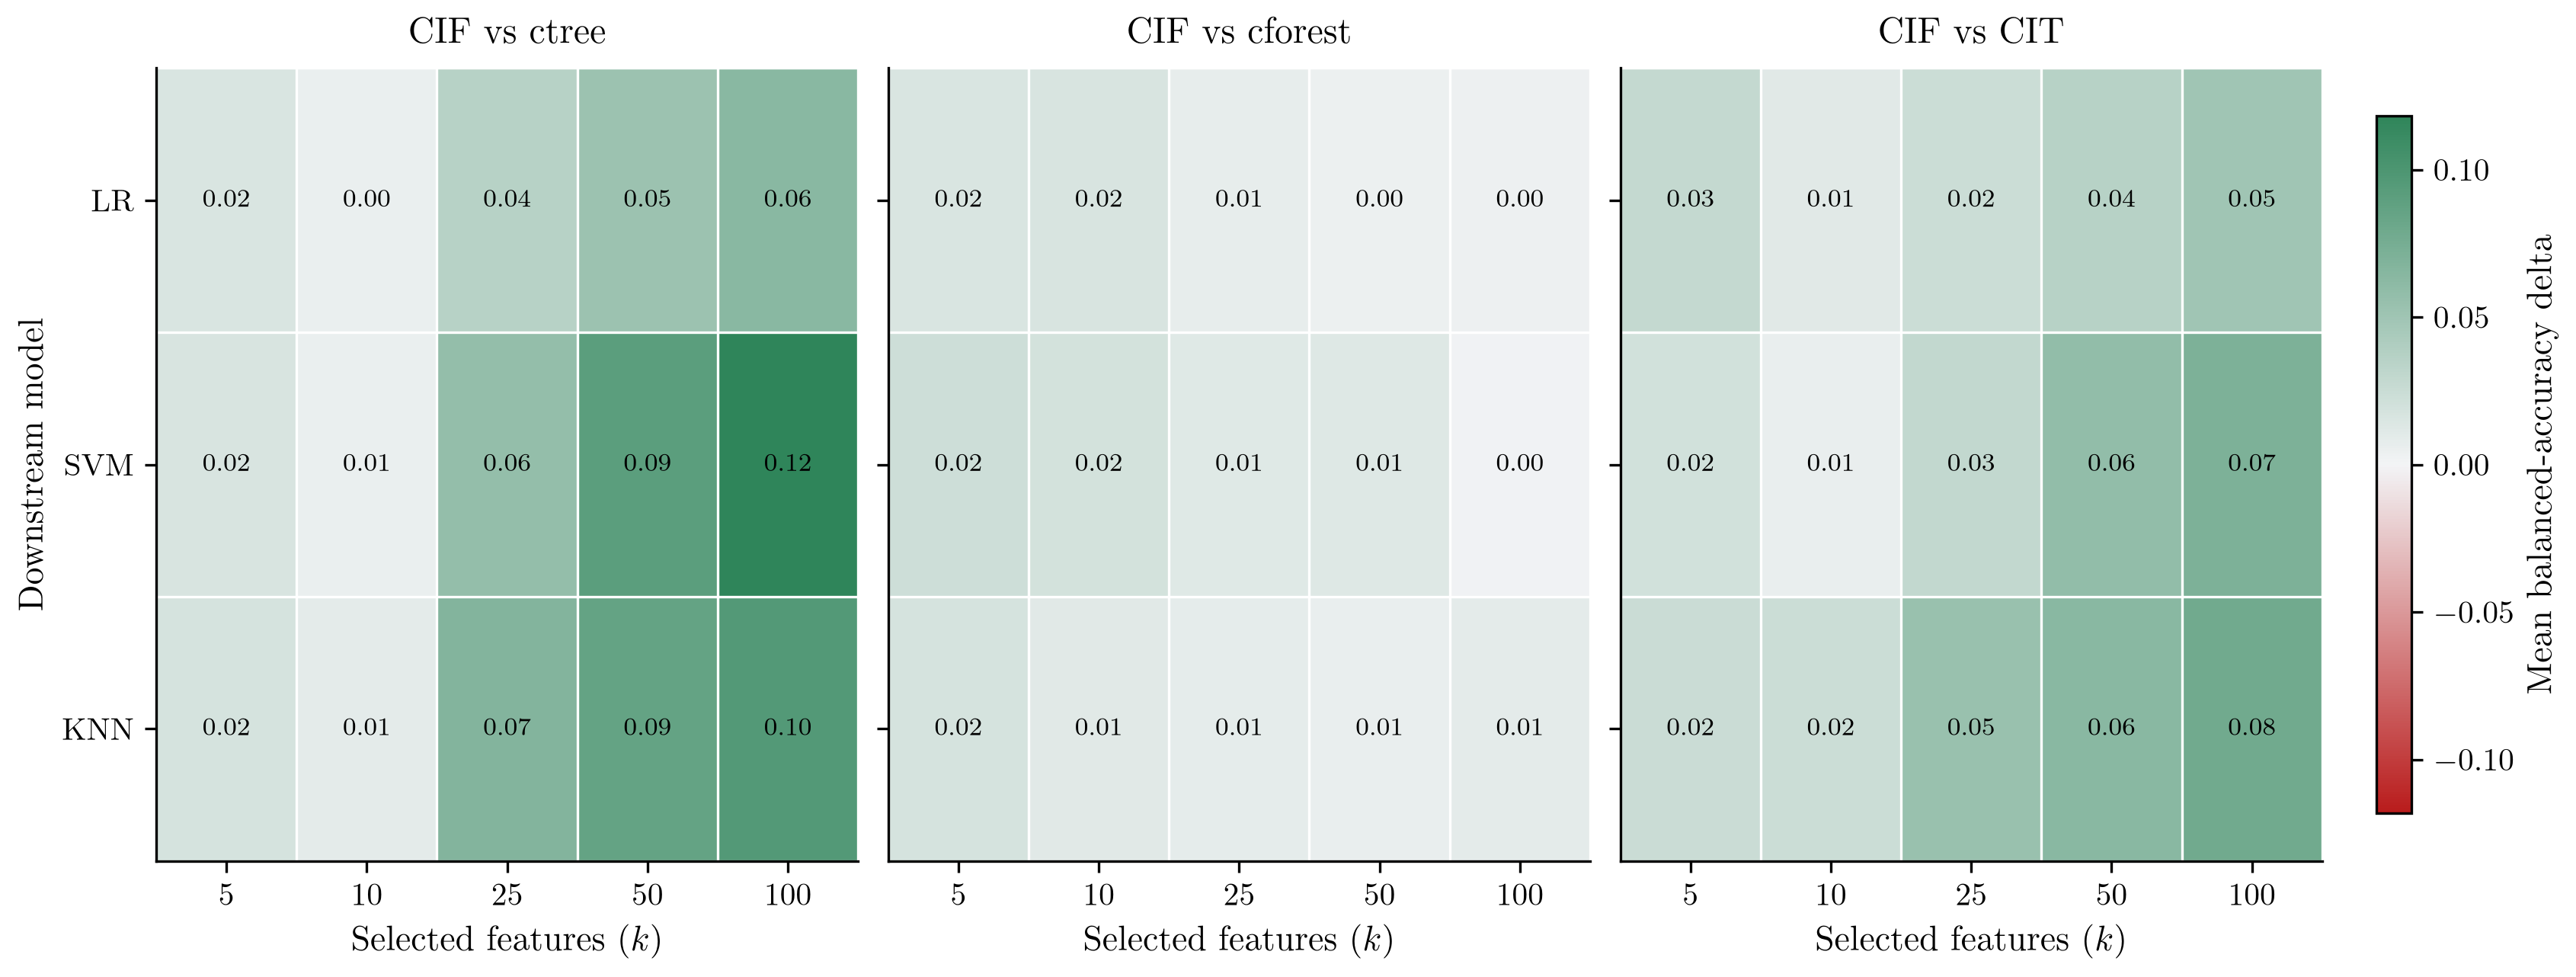
\includegraphics[width=0.88\linewidth]{figures/benchmark_pairwise_sensitivity.png}
  \caption{Classification CIF margins against ctree, cforest, and CIT by
  downstream learner and value of $k$. Each plotted value is the
  mean balanced-accuracy difference, CIF minus comparator, for one
  downstream learner and one value of $k$; positive values favor CIF. Dataset
  counts by $k$ are 21, 20, 14, 14, and 13 for ctree, 22, 21, 15, 15, and 14
  for cforest, and 23, 22, 16, 16, and 15 for CIT. Values are means over datasets; the bootstrap intervals for the pooled differences are in \cref{tab:conditional-inference-comparisons}.}
  \label{fig:benchmark-pairwise-sensitivity}
\end{figure}

\begin{figure}[tb]
  \centering
  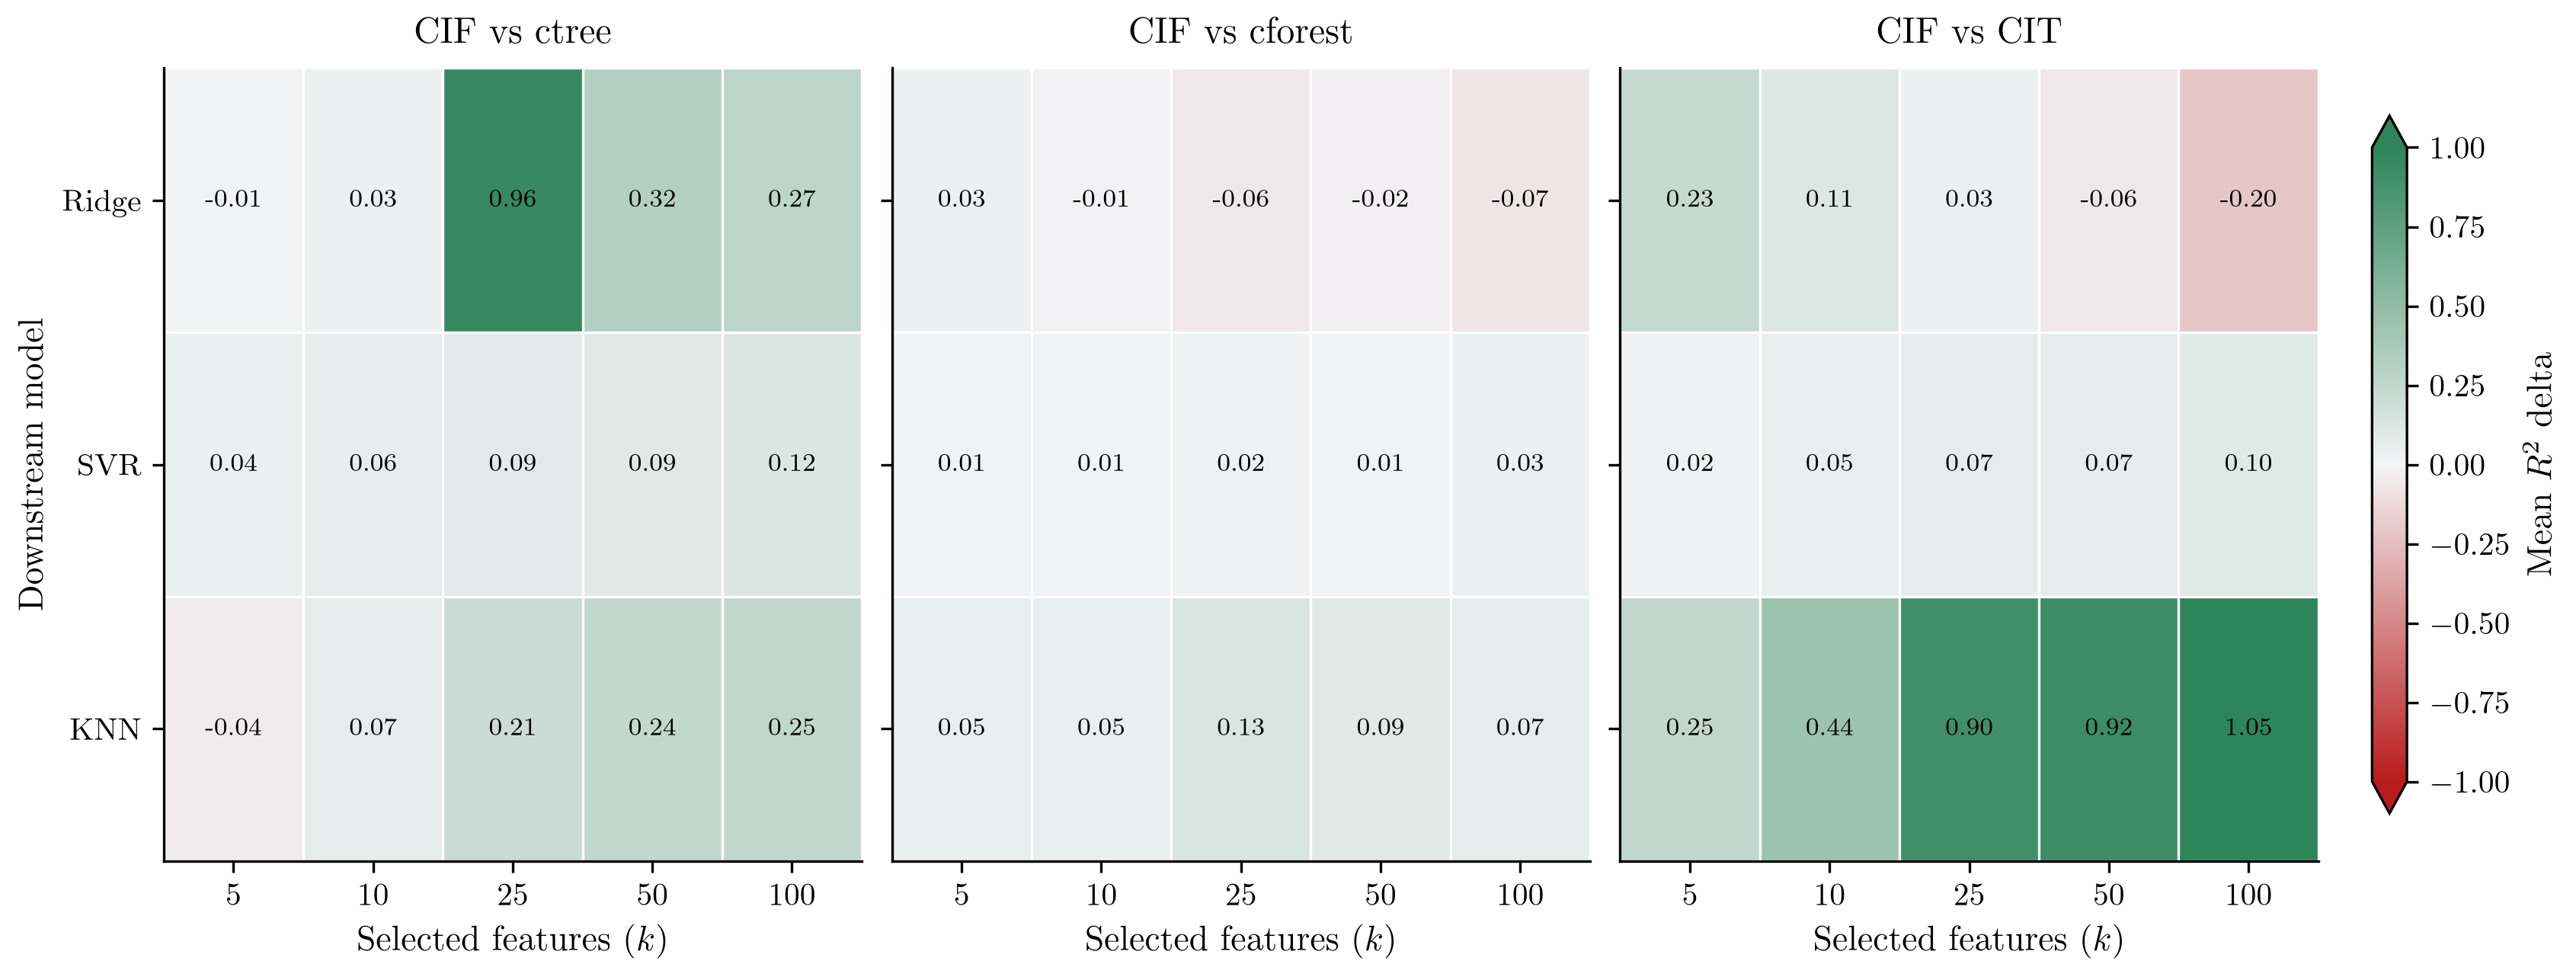
\includegraphics[width=0.88\linewidth]{figures/regression_benchmark_pairwise_sensitivity.png}
  \caption{Regression CIF margins against ctree, cforest, and CIT by
  downstream learner and value of $k$. Each plotted value is the mean
  $R^2$ difference, CIF minus comparator, for one downstream
  learner and one value of $k$; positive values favor CIF. Dataset counts by
  $k$ are 8, 8, 7, 7, and 6 for each comparison. Large positive plotted values
  can reflect negative mean $R^2$ for the comparator. Numeric labels show the
  unclipped values; the color scale is clipped at $\pm1$ for readability. Values are means over datasets; the bootstrap intervals for the pooled differences are in \cref{tab:conditional-inference-comparisons}.}
  \label{fig:regression-benchmark-pairwise-sensitivity}
\end{figure}

For the seed checks, each method is ranked separately within each fixed seed.
Keeping only datasets with results for every method, downstream learner,
standard top-$k$ value, and seed leaves 13 classification datasets and 6
regression datasets complete across all five seeds. These tables summarize seed
variation by rank without intervals or tests. In these tables, a seed column is
the method's ordinal position after sorting that seed's averaged dataset-level
ranks, while mean rank is the averaged dataset-level rank value itself. Rows
follow the main benchmark order. In classification CIF is 5th to 7th in every
seed (\cref{tab:classification-seed-sensitivity}), and in regression its
position ranges from 4th to 8th (\cref{tab:regression-seed-sensitivity}).

\begin{table}[tb]
  \centering
  \footnotesize
  \setlength{\tabcolsep}{4pt}
  \renewcommand{\arraystretch}{1.04}
  \begin{tabular}{@{}l
    S[table-format=2.0]
    S[table-format=2.0]
    S[table-format=2.0]
    S[table-format=2.0]
    S[table-format=2.0]
    S[table-format=2.1]
    S[table-format=2.1]@{}}
    \toprule
    \tablehead{Method} & {Seed 1} & {Seed 2} & {Seed 3} & {Seed 4} & {Seed 5} & {Mean position} & {Mean rank} \\
    \midrule
    RF-RFE & 1 & 1 & 1 & 1 & 1 & 1.0 & 4.9 \\
    XGBoost & 2 & 4 & 2 & 3 & 3 & 2.8 & 5.8 \\
    CIF & 6 & 5 & 6 & 5 & 7 & 5.8 & 6.9 \\
    RF & 5 & 6 & 4 & 6 & 4 & 5.0 & 6.6 \\
    LightGBM & 3 & 2 & 3 & 2 & 2 & 2.4 & 5.6 \\
    Boruta & 7 & 7 & 8 & 7 & 8 & 7.4 & 7.6 \\
    CatBoost & 4 & 3 & 5 & 4 & 5 & 4.2 & 6.4 \\
    ExtraTrees & 8 & 8 & 7 & 8 & 6 & 7.4 & 7.5 \\
    cforest & 9 & 9 & 9 & 9 & 9 & 9.0 & 8.3 \\
    DT & 10 & 10 & 11 & 10 & 10 & 10.2 & 9.6 \\
    RDC filter & 11 & 11 & 12 & 13 & 12 & 11.8 & 10.4 \\
    PI & 16 & 16 & 16 & 16 & 16 & 16.0 & 14.2 \\
    MC filter & 13 & 14 & 14 & 14 & 15 & 14.0 & 11.1 \\
    RT & 15 & 15 & 15 & 15 & 14 & 14.8 & 11.6 \\
    ctree & 14 & 12 & 10 & 12 & 11 & 11.8 & 10.4 \\
    CIT & 12 & 13 & 13 & 11 & 13 & 12.4 & 10.5 \\
    CPI & 17 & 17 & 17 & 17 & 17 & 17.0 & 15.7 \\
    \bottomrule
  \end{tabular}
  \caption{Classification seed sensitivity on the 13 datasets complete across
  all five seeds. Each seed column is the method's ordinal position after
  sorting methods by their averaged dataset-level ranks for that seed. Mean
  position averages those five ordinal positions; mean rank reports the averaged
  dataset-level rank value itself. Lower values are better. The spread across seed columns is the reported sensitivity.}
  \label{tab:classification-seed-sensitivity}
\end{table}

\begin{table}[tb]
  \centering
  \footnotesize
  \setlength{\tabcolsep}{4pt}
  \renewcommand{\arraystretch}{1.04}
  \begin{tabular}{@{}l
    S[table-format=2.0]
    S[table-format=2.0]
    S[table-format=2.0]
    S[table-format=2.0]
    S[table-format=2.0]
    S[table-format=2.1]
    S[table-format=2.1]@{}}
    \toprule
    \tablehead{Method} & {Seed 1} & {Seed 2} & {Seed 3} & {Seed 4} & {Seed 5} & {Mean position} & {Mean rank} \\
    \midrule
    ExtraTrees & 3 & 2 & 3 & 3 & 3 & 2.8 & 7.4 \\
    CIF & 6 & 5 & 8 & 8 & 4 & 6.2 & 8.6 \\
    CatBoost & 2 & 7 & 4 & 1 & 1 & 3.0 & 7.4 \\
    RF-RFE & 1 & 1 & 1.5 & 4 & 2 & 1.9 & 7.2 \\
    RF & 5 & 3 & 5 & 7 & 7 & 5.4 & 8.5 \\
    RT & 4 & 4 & 1.5 & 5 & 6 & 4.1 & 8.2 \\
    cforest & 15 & 13 & 13 & 12 & 11 & 12.8 & 10.2 \\
    DT & 14 & 6 & 7 & 2 & 5 & 6.8 & 8.6 \\
    Boruta & 9 & 10 & 10 & 11 & 8 & 9.6 & 9.3 \\
    PC filter & 16 & 16 & 15 & 14 & 16 & 15.4 & 11.3 \\
    LightGBM & 8 & 9 & 9 & 10 & 10 & 9.2 & 9.3 \\
    XGBoost & 7 & 8 & 11 & 6 & 12 & 8.8 & 9.2 \\
    RDC filter & 10 & 14 & 14 & 13 & 14 & 13.0 & 10.4 \\
    CIT & 12 & 12 & 17 & 17 & 9 & 13.4 & 10.7 \\
    ctree & 13 & 15 & 12 & 15 & 13 & 13.6 & 10.6 \\
    PI & 11 & 11 & 6 & 9 & 15 & 10.4 & 9.7 \\
    DC filter & 17 & 17 & 16 & 16 & 17 & 16.6 & 11.9 \\
    CPI & 18 & 18 & 18 & 18 & 18 & 18.0 & 12.8 \\
    \bottomrule
  \end{tabular}
  \caption{Regression seed sensitivity on the 6 datasets complete across all
  five seeds. Each seed column is the method's ordinal position after sorting
  methods by their averaged dataset-level ranks for that seed; fractional
  positions indicate ties. Mean position
  averages those five ordinal positions; mean rank reports the averaged
  dataset-level rank value itself. Lower values are better. The spread across seed columns is the reported sensitivity.}
  \label{tab:regression-seed-sensitivity}
\end{table}

\section{Where CIF is weaker}
\label{app:weaker}

\Cref{fig:high-p-boundary} shows, by downstream learner, where the
classification scores of CIF peak on the 15 datasets with more than 100
features, the pattern summarized in \cref{sec:boundary}. Scores peak at
intermediate $k$ ($100<k<p$) on 8 of 15 LR datasets, 12 of 15 SVM datasets, and
9 of 15 KNN datasets.

\begin{figure}[tb]
  \centering
  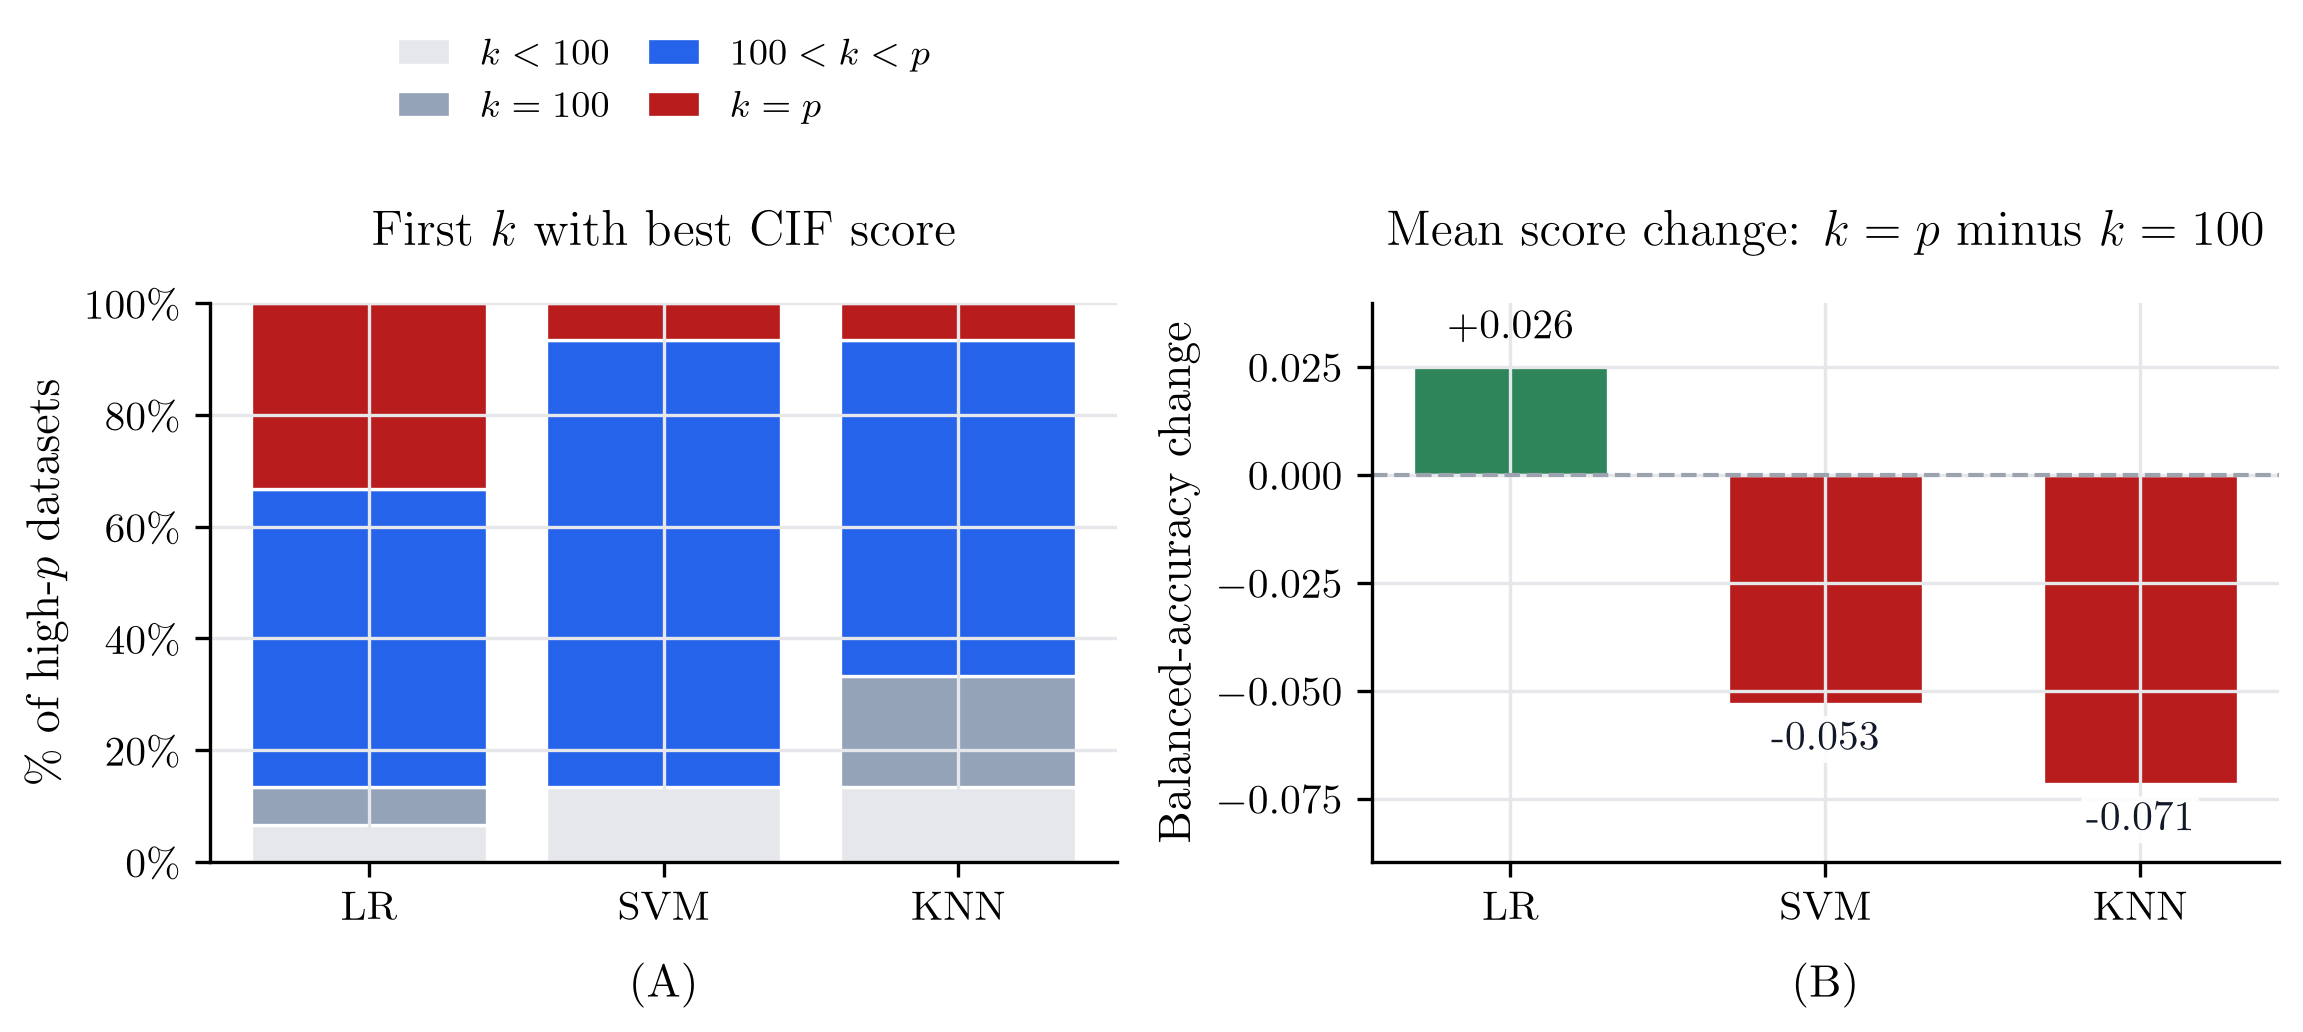
\includegraphics[width=0.84\linewidth]{figures/high_p_boundary_summary.png}
  \caption{Where CIF's classification scores peak as $k$ increases, by
  downstream learner. (A) shows, for each learner, the percentage of 15
  datasets where the first evaluated $k$ attaining the best observed CIF score
  falls below 100, at 100, between 100 and $p$, or at $k=p$. (B) shows the mean
  balanced accuracy change from $k=100$ to $k=p$.}
  \label{fig:high-p-boundary}
\end{figure}

\subsection{Synthetic recovery by \texorpdfstring{$k$}{k}}

\Cref{fig:synthetic-topk-curves} shows synthetic recovery as $k$ grows for
CIT, the forests, and the boosted trees, the curves behind the averages over
$k$ in \cref{tab:synthetic-head}.

\begin{figure}[tb]
  \centering
  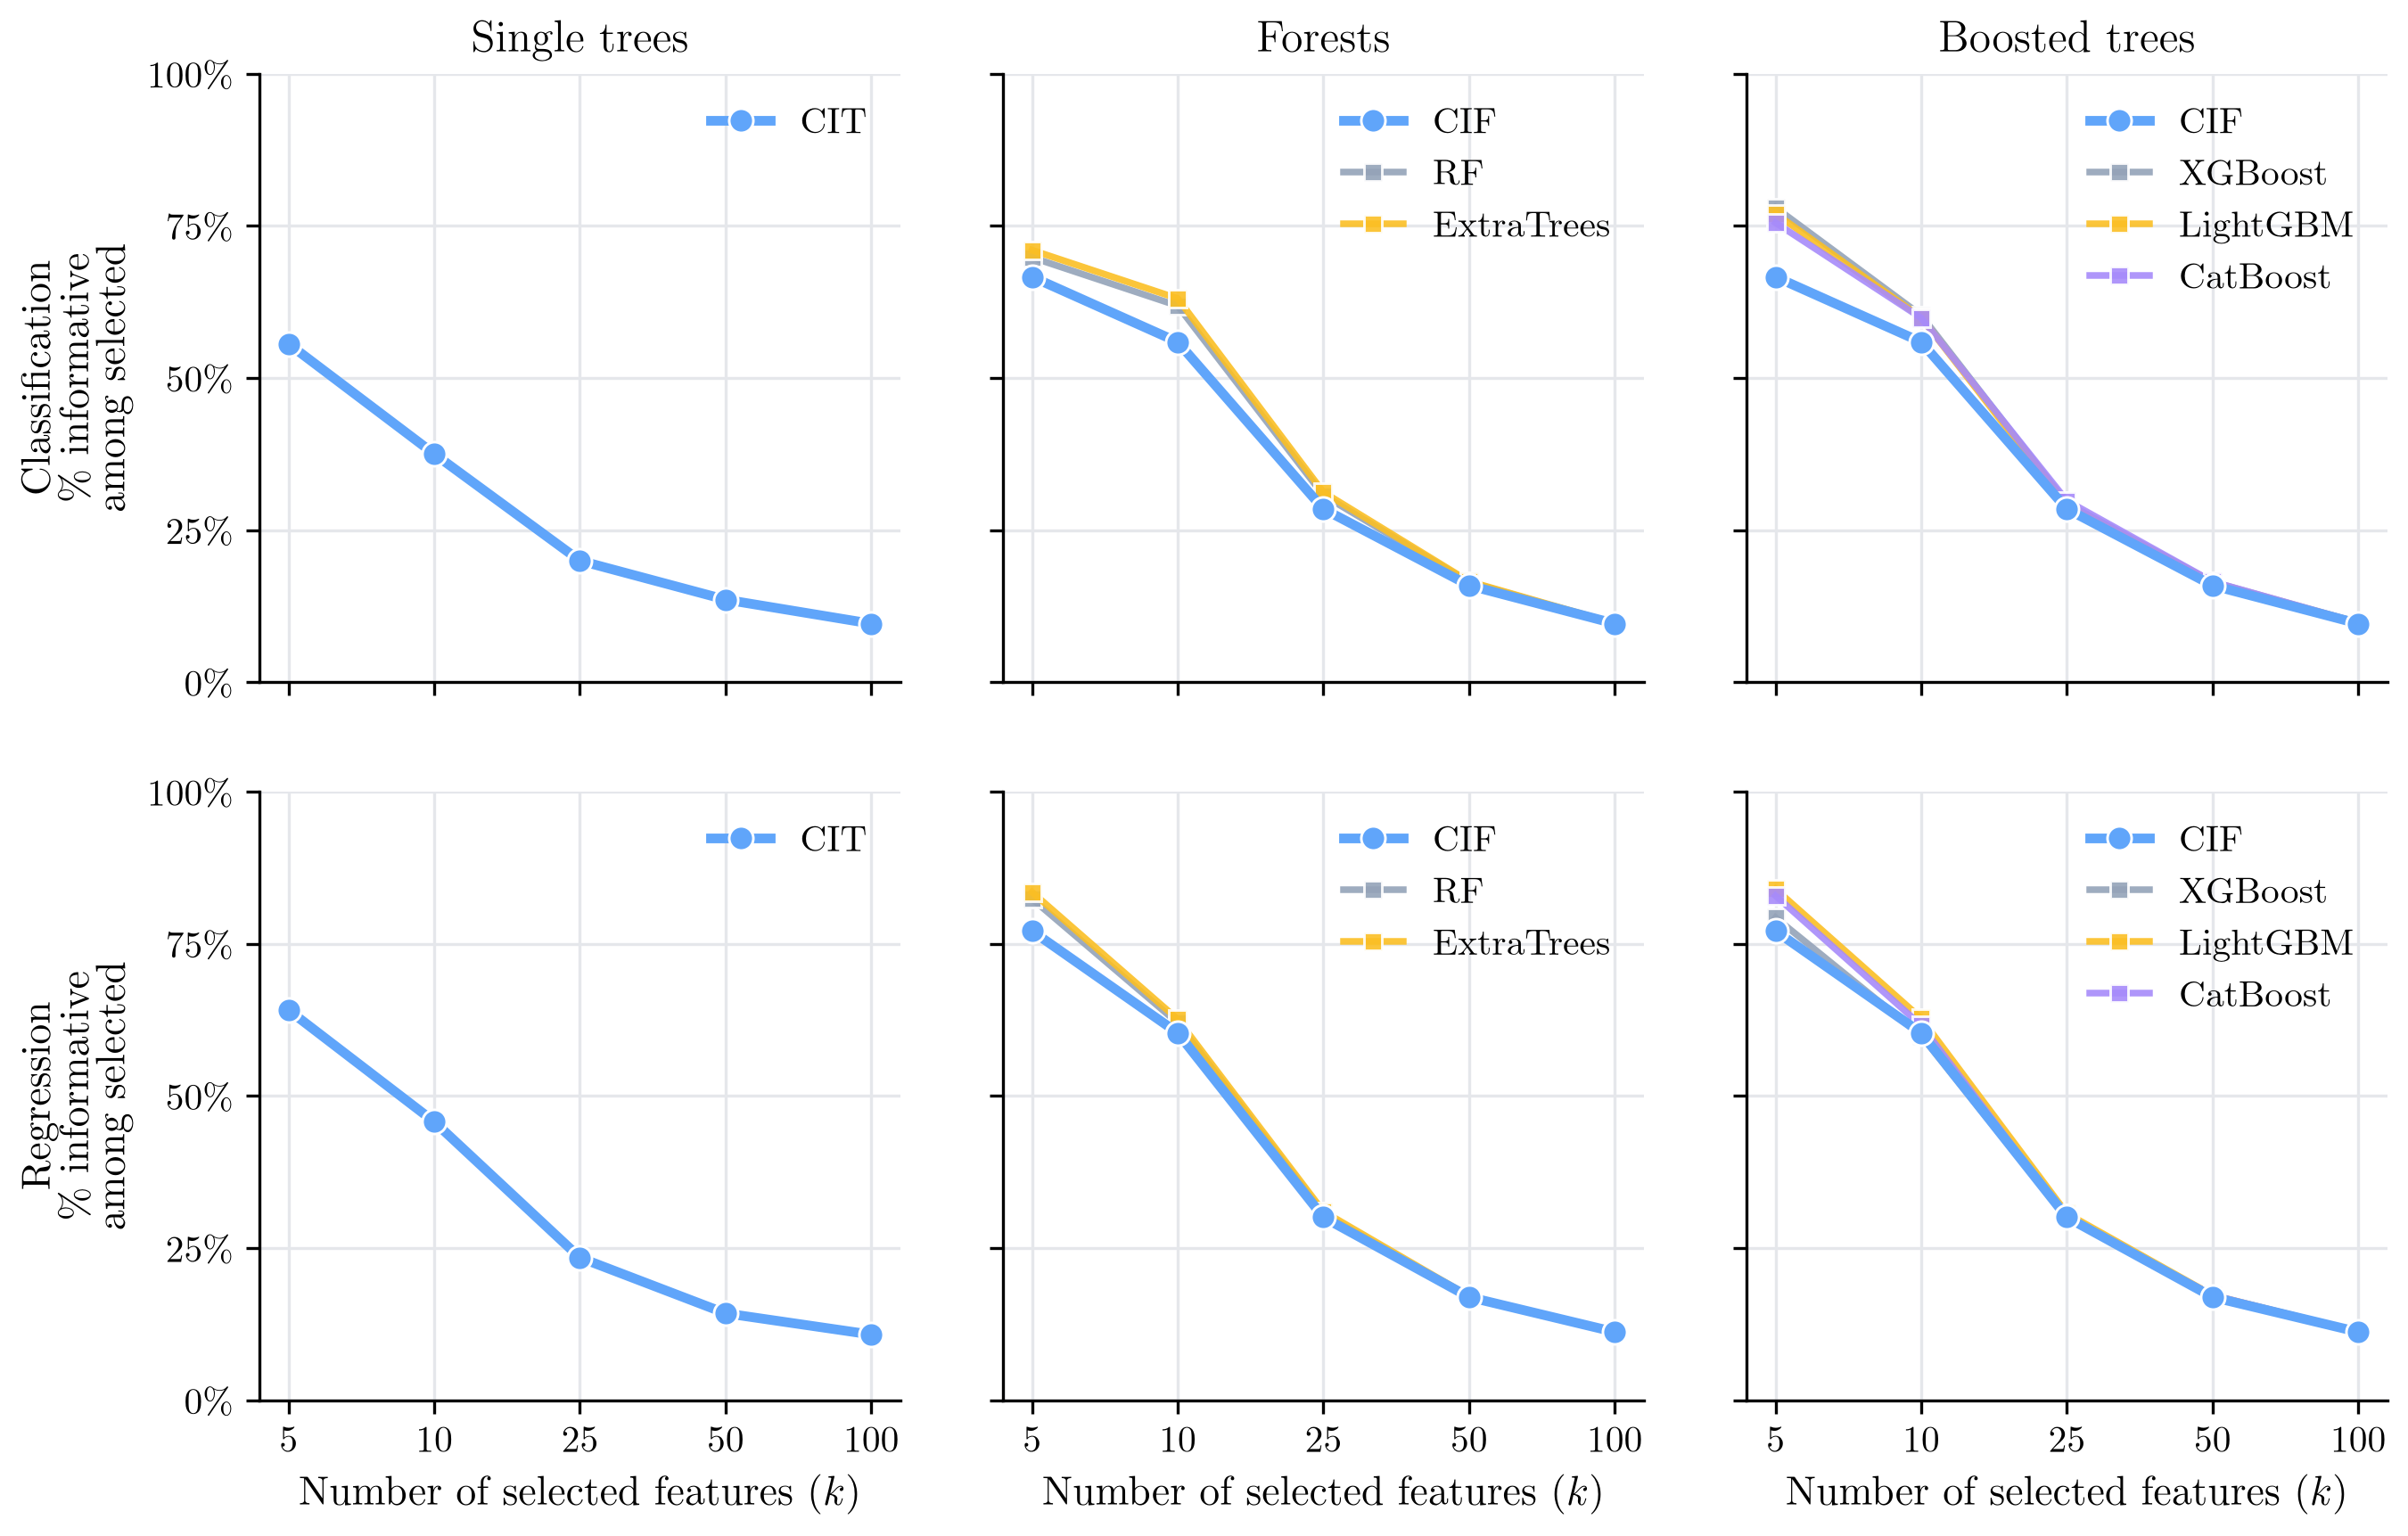
\includegraphics[width=0.84\linewidth]{figures/synthetic_topk_focus_curves.png}
  \caption{Synthetic top-$k$ recovery curves. Columns show CIT alone, then CIF
  against the forests and against the boosted trees; rows show classification
  and regression. Each
  value is the percentage of selected features that are truly informative.}
  \label{fig:synthetic-topk-curves}
\end{figure}

\subsection{Feature use in sampled forests}
\label{app:candidate-availability}

\Cref{sec:mechanism} measures feature use by comparing CIF with CIF-all, which
keeps feature muting and the other tree settings unchanged while removing
feature subsampling. \Cref{fig:candidate-forest-counts} shows how many trees
use each feature in the design with two informative features among 1,000.
CIF-all splits on one informative feature in every tree and on no
uninformative feature, while CIF, RF, and ExtraTrees spread their splits over
the uninformative columns; in that design CIF uses an informative feature in
9.0\% of splits, RF in 2.7\%, ExtraTrees in 2.0\%, and CIF-all in 100.0\%.
Across $p \in \{100,500,1{,}000\}$ with 1,000 trees per fit, evaluating all
nonconstant features raises the share of splits on informative features most
in the sparse high-$p$ classification settings: with two informative features,
CIF uses informative features in 40.0, 12.2, and 9.0\% of splits at $p=100$,
500, and 1,000, against 100.0, 90.2, and 100.0\% for CIF-all. Regression shows a
similar pattern when one or two features are informative, with a smaller
average gain, 42.3\% of splits on informative features for CIF-all against
27.8\% for CIF. The curves by $p$, with the counts of distinct uninformative
features each forest uses, follow in \cref{app:feature-use-dimension}.

\begin{figure}[tb]
  \centering
  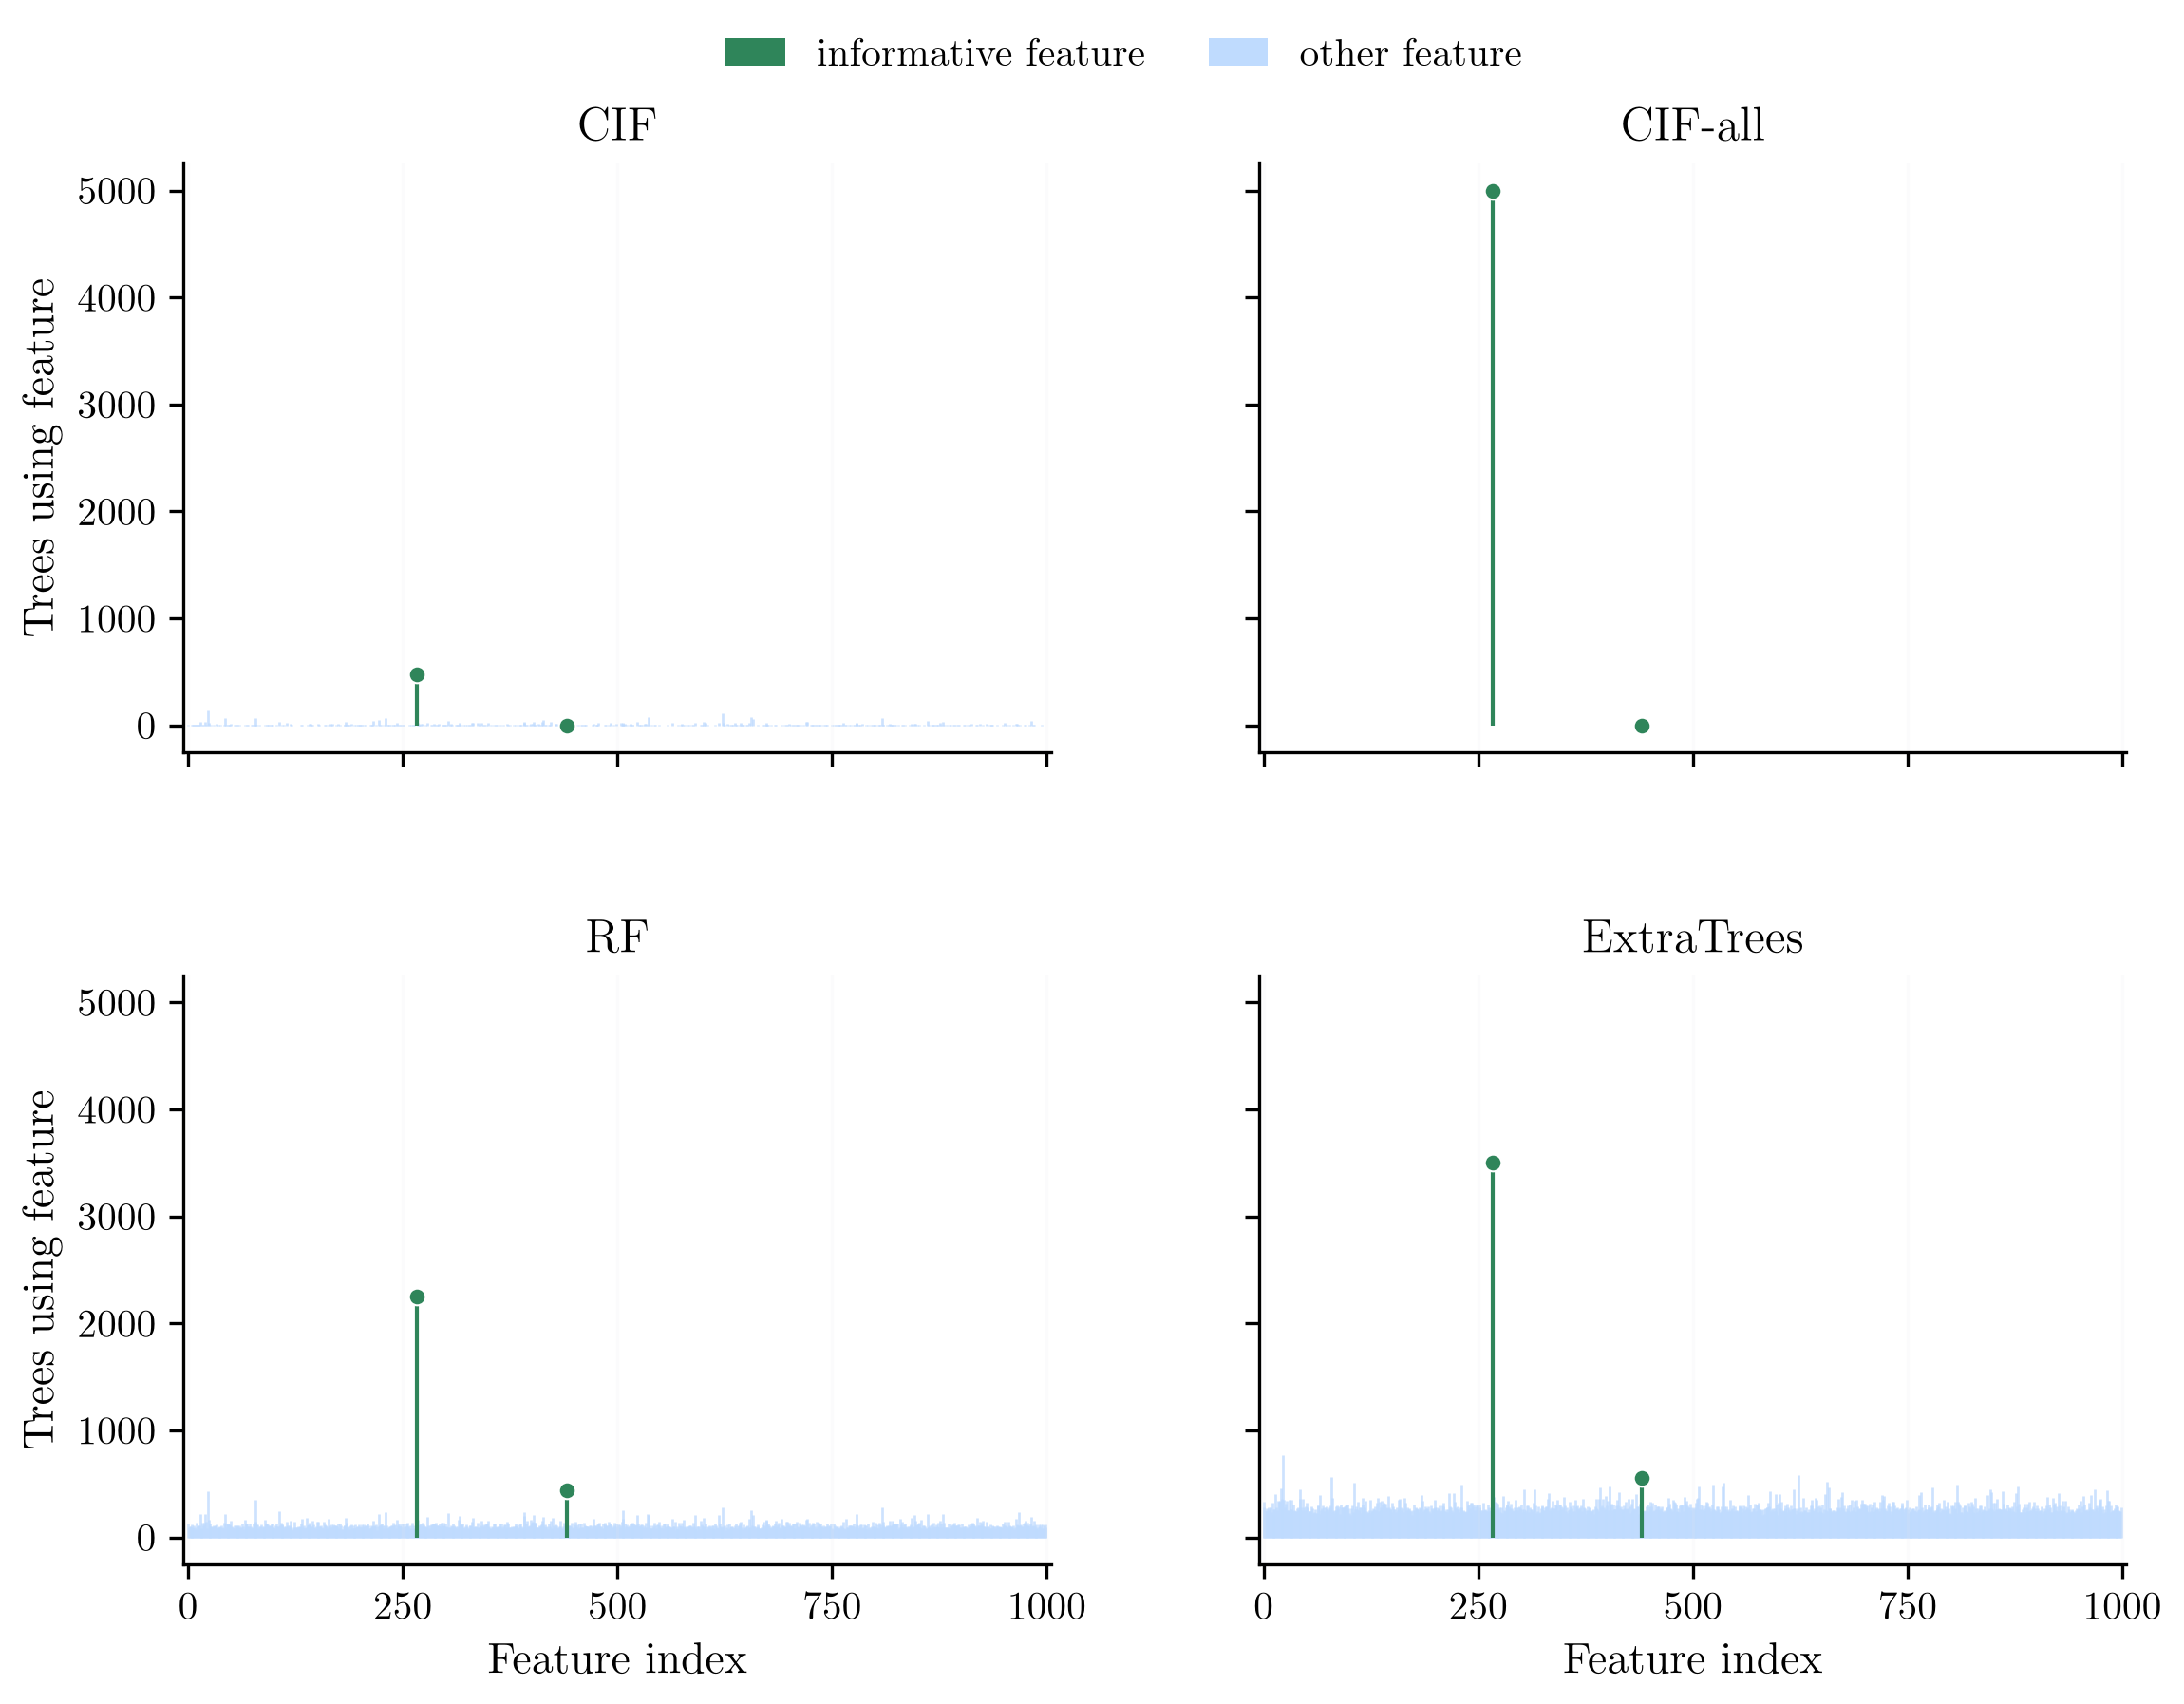
\includegraphics[width=0.84\linewidth]{figures/paper_mechanism_grid_forest_classification_feature_counts_p1000_i2_1000trees.png}
  \caption{Tree-level feature use in one sparse classification forest design
  ($n=250$, $p=1{,}000$, two informative features). Counts are the number of
  trees using each feature in at least one split, pooled over five fits of
  1,000 trees each, so the shared vertical axis runs to 5,000. CIF samples a
  subset of features at each node; CIF-all evaluates all nonconstant
  features.}
  \label{fig:candidate-forest-counts}
\end{figure}

\subsection{Feature use by feature dimension}
\label{app:feature-use-dimension}

\Cref{fig:candidate-dimension-curves} gives the feature-use curves behind
\cref{app:candidate-availability}, for $p \in \{100,500,1{,}000\}$ with 1,000
trees per fit. Each point is the mean over
$n_{\mathrm{informative}} \in \{1,2,5,10\}$, and the capped bar spans the
minimum and maximum over those four sparse settings; the values quoted below
for one, two, or five informative features come from single designs in the same
runs. In classification, evaluating all nonconstant features also narrows the
set of uninformative features used: over the 12 designs CIF-all uses a mean of
93.4 distinct uninformative features against 265.1 for CIF, each counted over
the five pooled fits of a design. With two informative features, CIF-all uses
70, 264, and 439 fewer distinct uninformative features than CIF at $p=100$,
500, and 1,000 (totals over the pooled fits), and with five informative
features the CIF-all minus CIF differences in the share of informative splits
are 25.1, 56.4, and 54.3\%. In regression, CIF-all uses more distinct
uninformative features than CIF, a mean of 528.8 against 367.7. With two
informative features, CIF uses informative features in 39.9, 19.7, and 11.6\%
of regression splits at the three values of $p$, against 58.8, 46.7, and 35.9\%
for CIF-all, and with one informative feature the CIF-all minus CIF
differences are 29.8, 18.9, and 42.1\%.

\begin{figure}[tb]
  \centering
  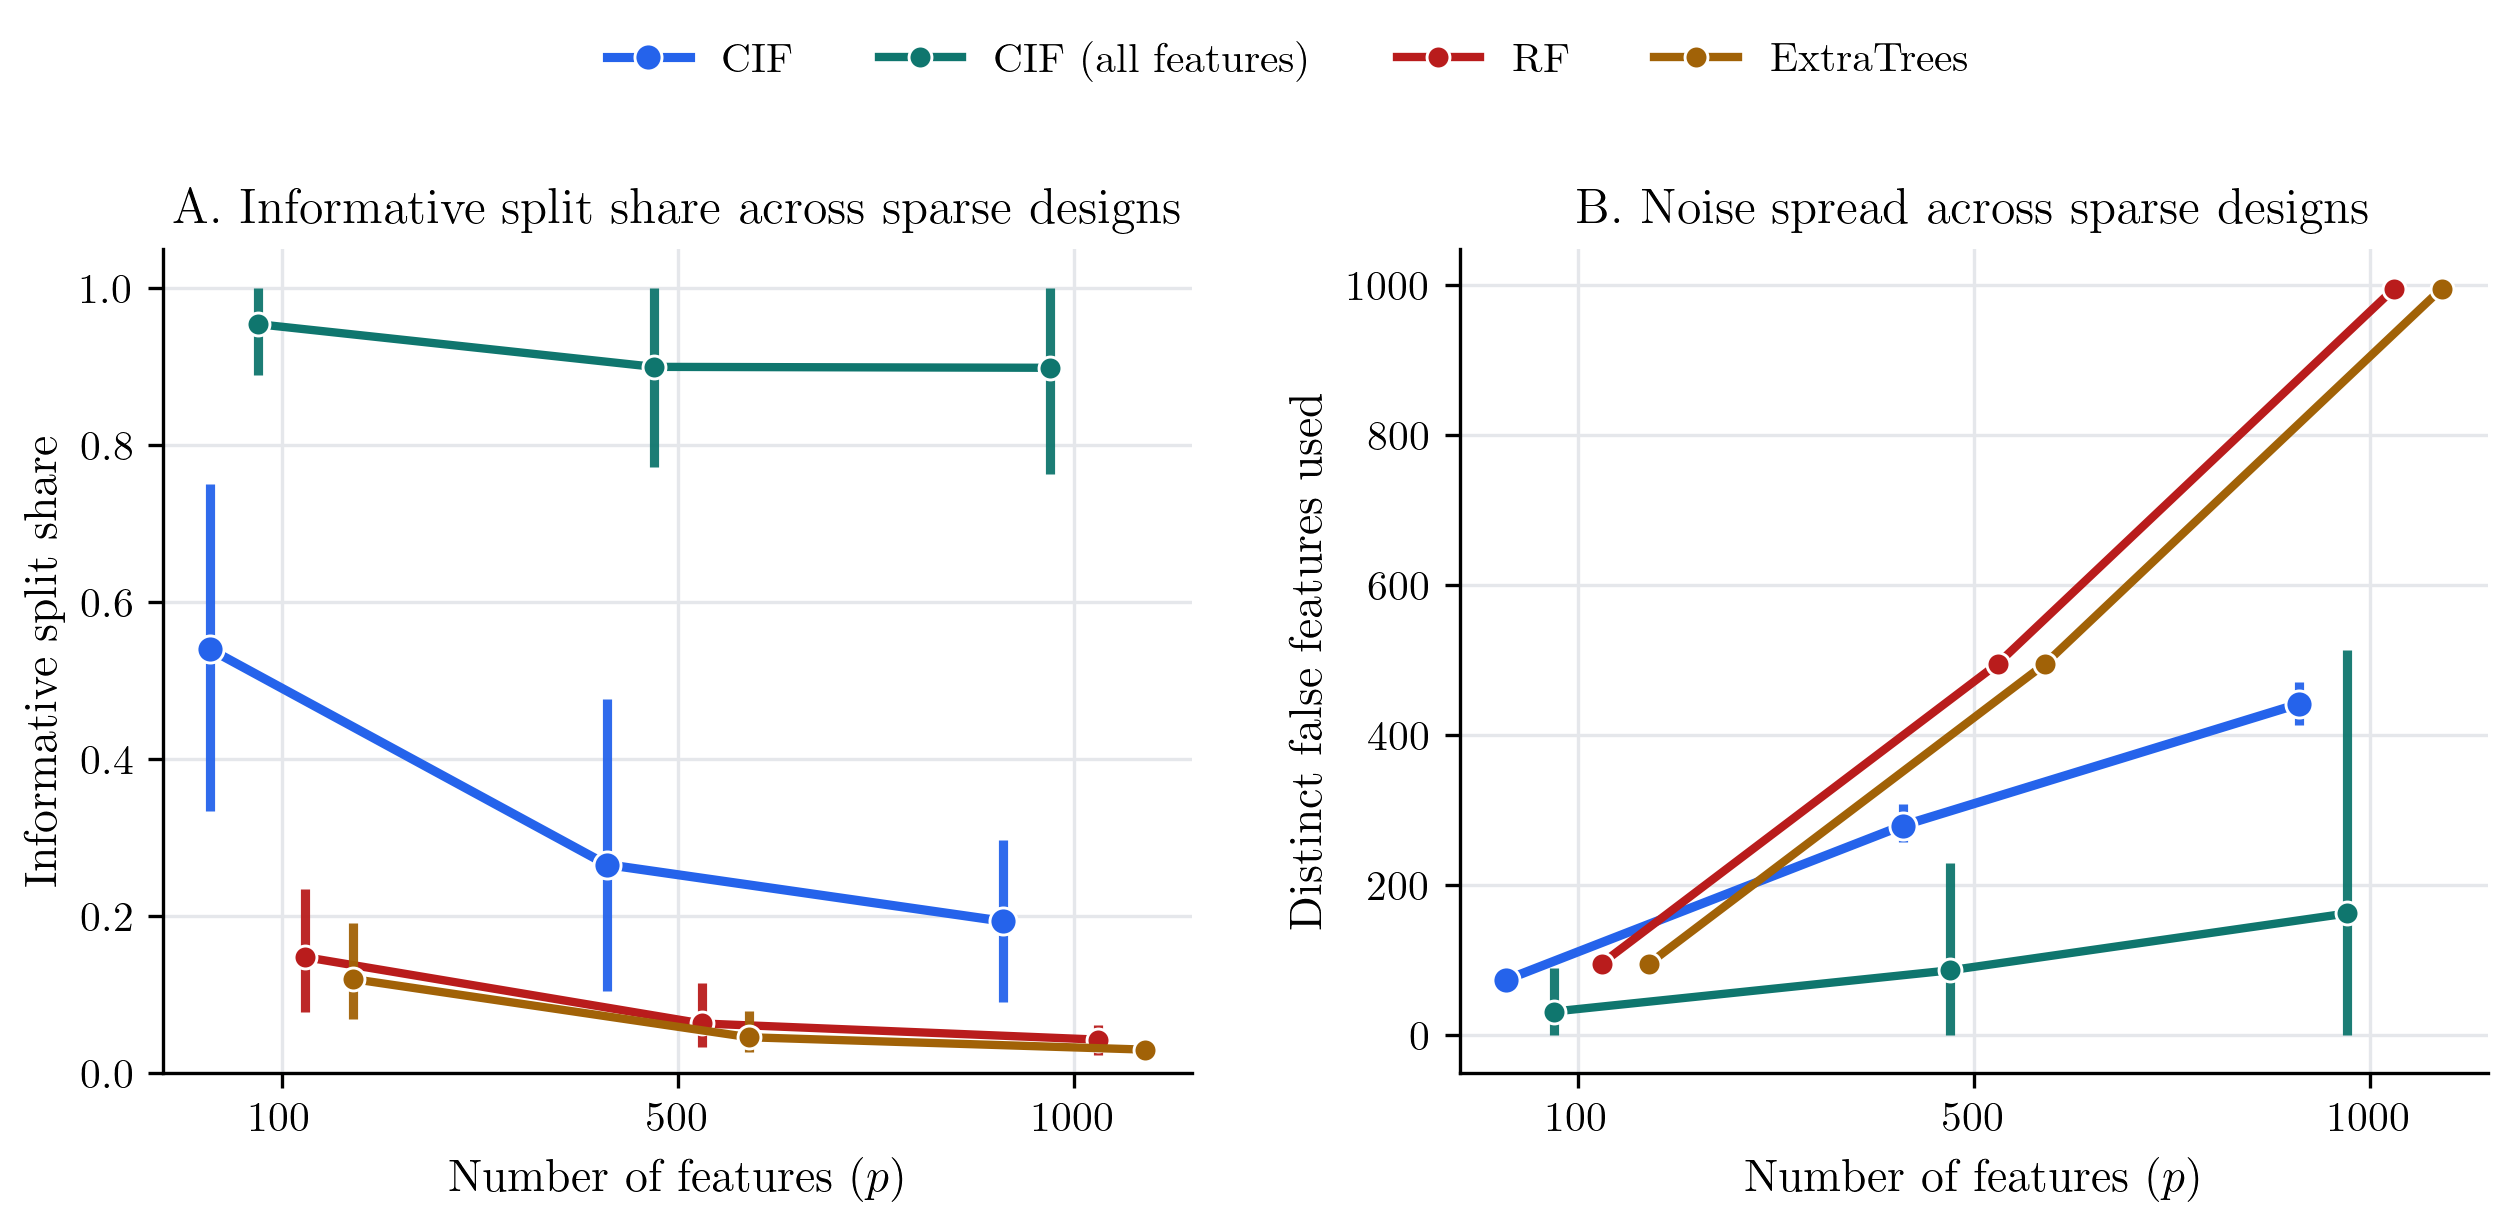
\includegraphics[width=0.88\linewidth]{figures/paper_mechanism_grid_forest_classification_dimension_curves_1000trees.png}\par
  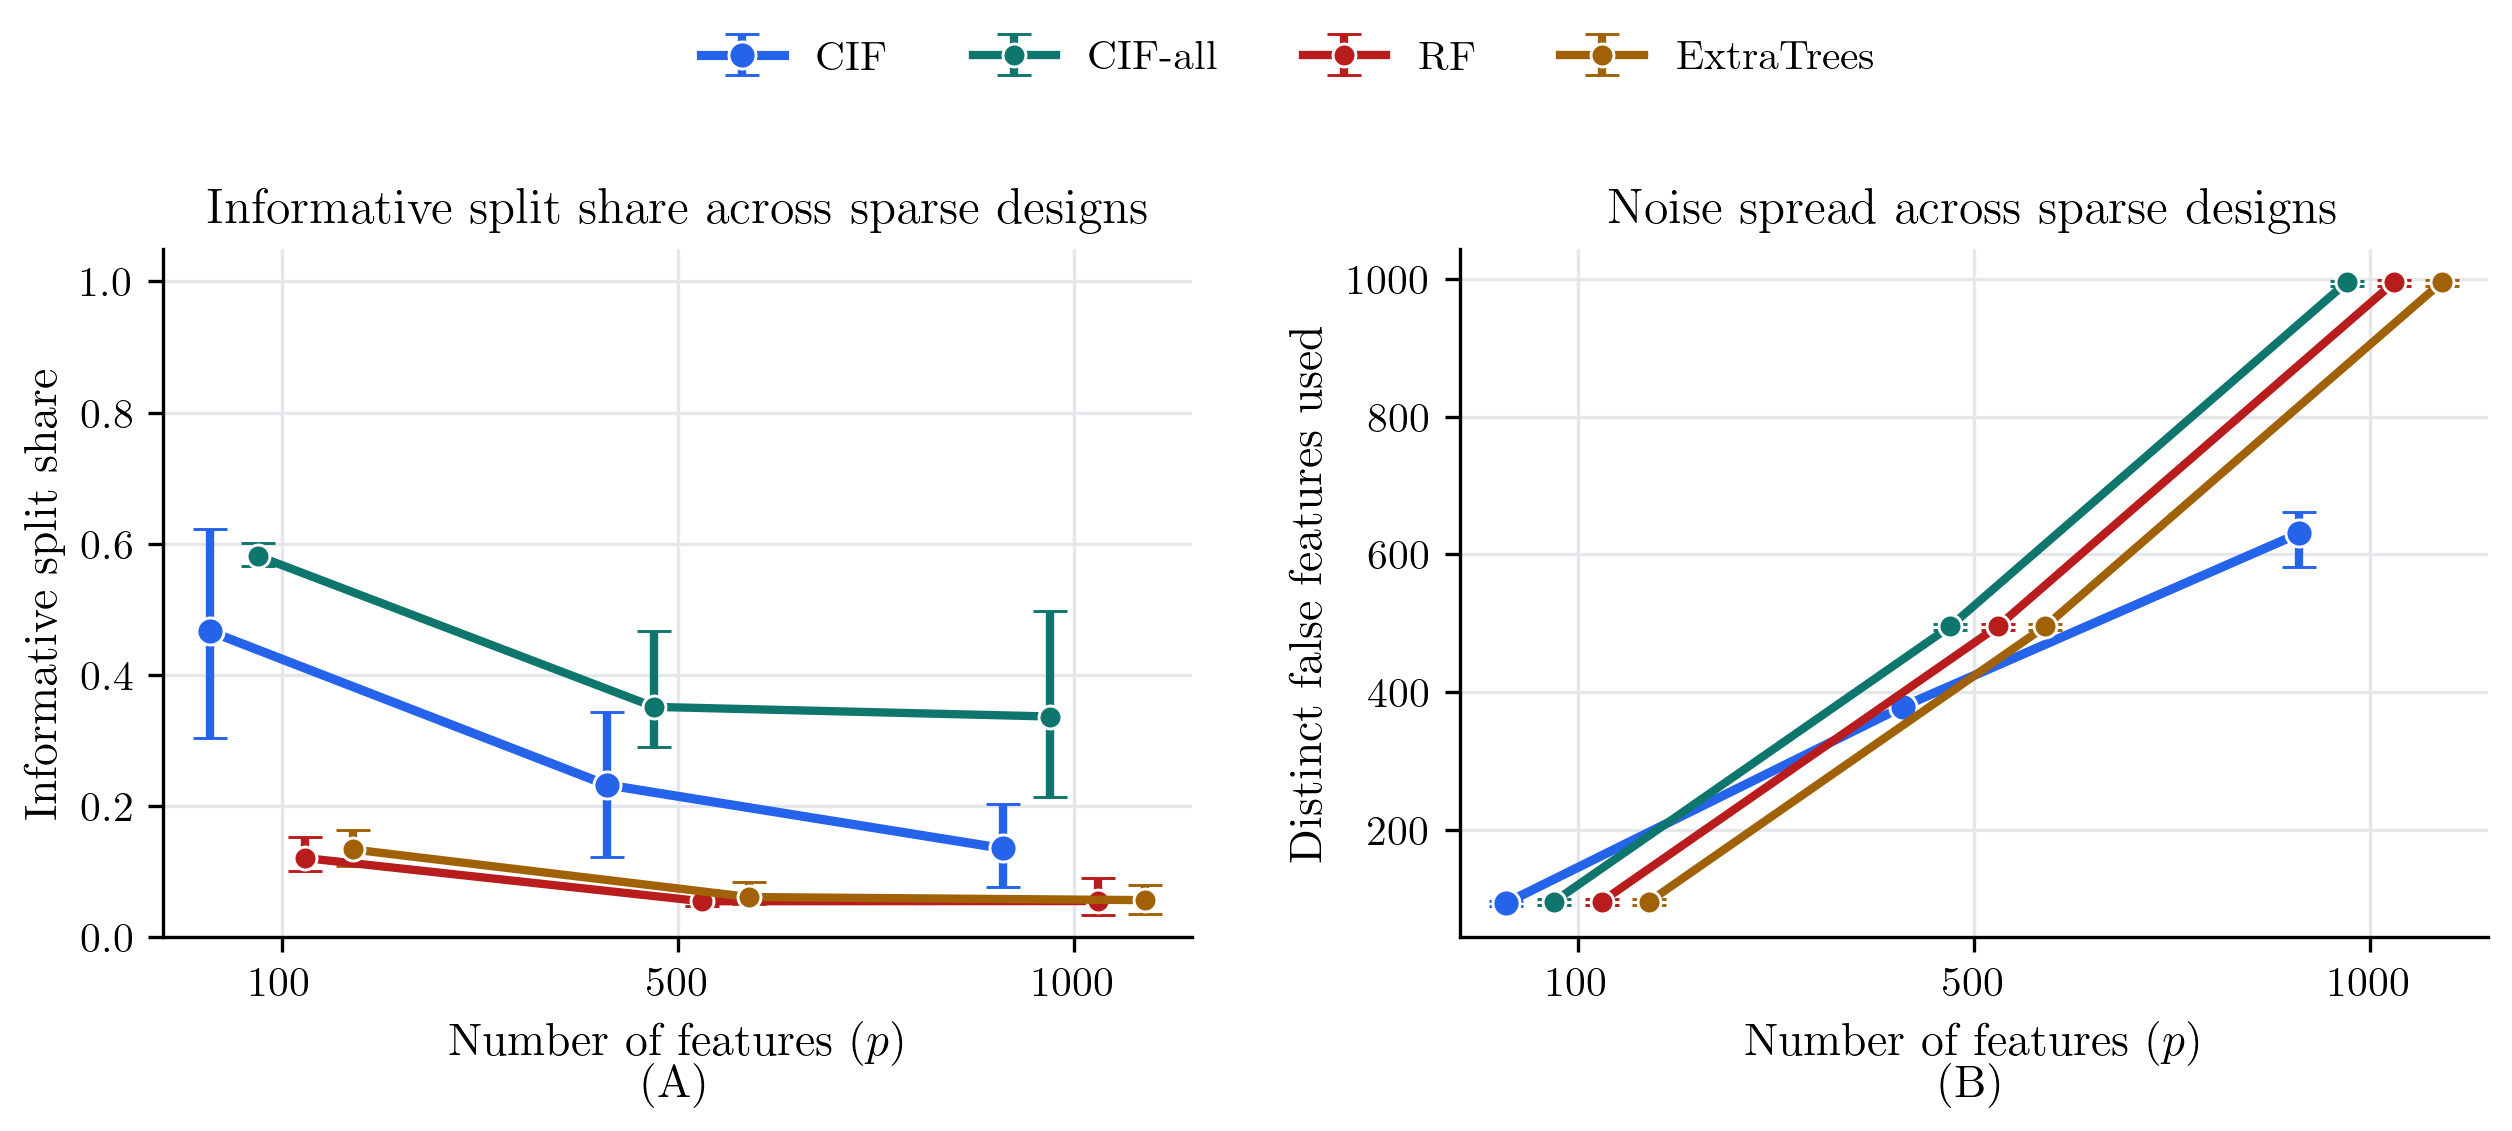
\includegraphics[width=0.88\linewidth]{figures/paper_mechanism_grid_forest_regression_dimension_curves_1000trees.png}
  \caption{Forest feature use by feature dimension $p$, for classification
  (top row) and regression (bottom row), with 1,000 trees per fit. Points are
  means over $n_{\mathrm{informative}} \in \{1,2,5,10\}$; capped bars span the
  minimum and maximum over those four sparse designs. In each row, (A) shows
  the percentage of splits using informative features and (B) the number of
  distinct uninformative features used. CIF samples a subset of features at
  each node; CIF-all evaluates all nonconstant features.}
  \label{fig:candidate-dimension-curves}
  \label{fig:regression-candidate-dimension-curves}
\end{figure}

\section{Runtime and memory accounting}
\label{app:complexity-details}

\paragraph{Notation.}
The runtime of a fit is the sum, over realized nodes, of the scans, copies, and
tests each node reaches. Let $n$ be the training sample count and $p$ the
number of features. At node $t$, $n_t$ samples arrive,
$a_t=|F_{t,\mathrm{avail}}|$ features are available, $d_t^{\mathrm{const}}$ of
them are constant, Stage~A considers $m_t=|F_t|$ features, and feature muting
removes $d_t^{\mathrm{mute}}$ tested features from the descendant pool. Stage~B
generates $\tilde{K}_t$ thresholds for $j_t^\star$, of which $K_t$ remain after
the minimum leaf size filter. Let $C^{\mathrm{sel}}_j(n_t)$ be the cost of one
Stage~A statistic and $C^{\mathrm{split}}(n_t)$ that of one weighted child
impurity, excluding label copies, shuffles, and masks. Both are linear in $n_t$
for the MC and PC selectors with Gini and MSE splitting; the RDC costs
$O(n_t\log n_t)$ for fixed projection count, and distance correlation
$O(n_t\log n_t)$ or $O(n_t^2)$ depending on the backend.

\paragraph{Per-node work.}
Every node pays $O(n_t)$ for the stopping checks and leaf value. A node that can
split pays $O(a_t n_t)$ to find constant features, $O(a_t d_t^{\mathrm{const}})$
to remove them, and $O(a_t d_t^{\mathrm{mute}})$ for muting, so feature
subsampling caps $m_t$ but not this pass. With $\mathcal{J}_t$ the Stage~A
features tested before the scan stops and $b^{\mathrm{sel}}_{t,j}$ the
permutations drawn for feature $j$, the Stage~A work is
\begin{equation}
  S^{\mathrm{A}}_t
  = O\!\left(\sum_{j \in \mathcal{J}_t}
      \bigl(b^{\mathrm{sel}}_{t,j}+1\bigr)
      \bigl(C^{\mathrm{sel}}_j(n_t)+n_t\bigr)\right),
\end{equation}
where the $+1$ is the observed statistic and the $n_t$ term covers label copies
and shuffles; feature scanning adds
$O(\sum_{j\in F_t} C^{\mathrm{sel}}_j(n_t) + m_t\log m_t)$ for the prescan and
sort. Stage~B builds its thresholds in $O(n_t\log n_t)$, because unique values
are sorted before any cap applies; exact search and features with at most four
unique values keep all midpoints. With $\mathcal{C}^{\mathrm{eval}}_t$ the
thresholds tested before the scan stops and $b^{\mathrm{split}}_{t,c}$ the
permutations drawn at threshold $c$, the Stage~B work has the form of
$S^{\mathrm{A}}_t$ with $C^{\mathrm{split}}(n_t)$ in place of
$C^{\mathrm{sel}}_j(n_t)$. At the minimum budget the per-threshold rule draws
$\lceil K_t/\alpha_{\mathrm{split}}\rceil$ permutations for each threshold,
and the max-type rule draws one set of $B$ permutations for all $K_t$
candidates, so
\begin{align*}
  \text{per-threshold rule:}\quad S^{\mathrm{B}}_t
  &= O\!\left(|\mathcal{C}^{\mathrm{eval}}_t|\,
      \lceil K_t/\alpha_{\mathrm{split}}\rceil
      \bigl(C^{\mathrm{split}}(n_t)+n_t\bigr)\right),\\
  \text{max-type rule:}\quad S^{\mathrm{B}}_t
  &= O\!\left((B+1)\,K_t\,\bigl(C^{\mathrm{split}}(n_t)+n_t\bigr)\right),
\end{align*}
where the $n_t$ term covers masks, child-label slices, copies, and shuffles.
The first is quadratic in the candidate count when every threshold is tested,
and the second is linear at fixed $B$. Threshold scanning adds
$O(K_t(C^{\mathrm{split}}(n_t)+n_t) + K_t\log K_t)$ for ordering, and an
accepted split copies the node data into two child matrices with all $p$
columns, at $O(n_t p)$. Adaptive stopping and the two scans reduce work only
when they shorten the realized path, so the worst case is still every feature,
every threshold, and the full budget. Under the corrections a stage of
$n_{\mathrm{tests}}$ tests at nominal level $\alpha_{\mathrm{stage}}$ has a
maximum budget of about $n_{\mathrm{tests}}^2/(4\alpha_{\mathrm{stage}}^2)$ per
test, and an explicit integer budget is multiplied by $n_{\mathrm{tests}}$.

\paragraph{Trees and forests.}
With $W_t$ the work at node $t$, a tree costs
$T_{\mathrm{tree}}=\sum_{t\in\mathcal{V}(\mathcal{T})} W_t$ over its realized
nodes, leaves included, and a binary tree has
$|\mathcal{V}(\mathcal{T})|=2|\mathcal{I}(\mathcal{T})|+1$ nodes for
$|\mathcal{I}(\mathcal{T})|$ internal splits. Honesty computes the node
sum on the structure subsample and adds $O(np)$ for the partition plus a leaf
re-estimation pass. A forest of $M$ trees, with $s_r$ samples for tree $r$
after bootstrap sampling, costs
\begin{equation}
  T_{\mathrm{forest}}
  = O(np) + \sum_{r=1}^{M}\bigl(O(s_r p) + T_{\mathrm{tree},r}\bigr) + O(Mp),
\end{equation}
plus the honesty and out-of-bag scoring passes when they are requested; this
is total work, and wall-clock time also depends on the worker count and load
balance across trees.

\paragraph{Memory.}
The dense matrices dominate the node-local workspaces of
$O(a_t+m_t+n_t+\tilde{K}_t)$ and the permutation buffers, of which a
fixed-budget test without stopping may store its $B$ permuted statistics.
Validation materializes an $O(np)$ matrix, and each accepted split
materializes children of combined size $O(n_t p)$. Because the parent keeps the
sibling child alive during depth-first recursion, peak single-tree memory is
$O(np + p\sum_{u\in\mathcal{P}} n_u)$ over the accepted splits $\mathcal{P}$ on
the active recursion stack, which is $O(np)$ for balanced growth. A forest runs
up to $w=\min(M,n_{\mathrm{jobs}})$ trees at once, so its peak holds $w$ such
workspaces, and fitted storage holds the node records of all trees and $O(Mp)$
per-tree arrays.

\subsection{Measured scaling in \texorpdfstring{$n$}{n} and \texorpdfstring{$p$}{p}}
\label{app:scaling-curves}

\Cref{tab:scaling-curves} reports fit-only time for one CIT and one 100-tree CIF
on Gaussian predictors with a weak planted signal, under the fixed benchmark
settings of \cref{sec:bootstrap} at
$\alpha_{\mathrm{sel}}=\alpha_{\mathrm{split}}=0.05$, with the MC selector and
Gini splitting in classification and the PC selector and MSE splitting in
regression; the forest adds square-root feature sampling. With at most 257 candidates and at most
5{,}140 permutations per threshold, the per-node cost is linear in $n_t$ up to the
$O(n_t \log n_t)$ threshold sort. A
64-fold increase in $n$ at $p=20$ costs the tree about 68 times in
classification and 110 times in regression, and the forest 65 to 77 times. A
25-fold increase in $p$ at $n=2{,}000$ costs the tree 21 and 44 times, because
every predictor is scored at the root and muting removes only failed
predictors, while the forest is flat or falling under square-root feature
sampling.

\begin{table}[tb]
  \centering
  \footnotesize
  \setlength{\tabcolsep}{5pt}
  \begin{tabular}{@{}rrrrrrrrrr@{}}
    \toprule
     & & \multicolumn{4}{c}{Classification} & \multicolumn{4}{c}{Regression} \\
    \cmidrule(lr){3-6}\cmidrule(l){7-10}
     & & \multicolumn{2}{c}{CIT} & \multicolumn{2}{c}{CIF} & \multicolumn{2}{c}{CIT} & \multicolumn{2}{c}{CIF} \\
    \cmidrule(lr){3-4}\cmidrule(lr){5-6}\cmidrule(lr){7-8}\cmidrule(l){9-10}
    $n$ & $p$ & Adaptive & None & Adaptive & None & Adaptive & None & Adaptive & None \\
    \midrule
    500 & 20 & 0.17 & 0.16 & 13.1 & 13.2 & 0.08 & 0.08 & 12.2 & 12.2 \\
    500 & 100 & 0.21 & 0.19 & 13.0 & 13.3 & 0.25 & 0.22 & 12.5 & 12.3 \\
    500 & 500 & 4.2 & 3.5 & 13.8 & 13.4 & 4.3 & 3.3 & 12.2 & 12.1 \\
    2,000 & 20 & 0.61 & 0.57 & 53.7 & 54.8 & 0.38 & 0.36 & 54.9 & 46.3 \\
    2,000 & 100 & 0.87 & 0.81 & 45.6 & 46.1 & 1.0 & 0.92 & 42.9 & 43.0 \\
    2,000 & 500 & 12.6 & 11.0 & 48.6 & 49.7 & 16.4 & 13.2 & 45.5 & 45.7 \\
    8,000 & 20 & 2.8 & 2.7 & 216 & 211 & 1.7 & 1.6 & 191 & 193 \\
    8,000 & 100 & 3.2 & 3.0 & 180 & 182 & 3.9 & 3.5 & 163 & 163 \\
    32,000 & 20 & 11.3 & 10.7 & 988 & 1,015 & 8.5 & 8.1 & 788 & 797 \\
    32,000 & 100 & 11.3 & 10.7 & 655 & 688 & 13.2 & 12.1 & 705 & 685 \\
    \bottomrule
  \end{tabular}
  \caption{Fit-only wall-clock seconds for one CIT and one 100-tree CIF in the
  configuration of \cref{app:scaling-curves}, with adaptive stopping (Adaptive)
  and with no stopping (None), on Gaussian predictors with a weak planted
  signal in five of them. Each entry is the median of two timed fits on two
  data draws, after one untimed fit of the same cell. The cells with $n \ge 8{,}000$ and
  $p=500$ were not run. Tree depth is unbounded, so the forest times are not
  comparable with the depth-3 forests of the head-to-head timing.}
  \label{tab:scaling-curves}
\end{table}

The adaptive stopping checks never end a test early at the minimum budget
(\cref{sec:theory-adaptive}), so the ratio of the time with adaptive stopping
to the time with no stopping measures their cost. It is 1.02 to 1.28 for the tree (median 1.07) and 0.95 to
1.18 for the forest (median 0.99), in line with the runtime ablations of
\cref{tab:runtime-ablations}. Each test pays a fixed cost for the checks, and a
single tree runs one Stage~A test per predictor at every node, so the tree
ratio grows with $p$, from 1.02 to 1.07 at $p=20$ to 1.15 to 1.28 at $p=500$.
On the 14 Benchmark-size datasets of \cref{sec:results-practical}, switching
adaptive stopping off changes tree time by 0.80 to 1.01 (medians 0.97 in
classification and 0.88 in regression) and forest time by 0.99 to 1.34
(medians 1.00 and 1.03). For the tree, threshold scanning saves a median 17
times in classification (45 times on spam and nothing on gisette, 0.96) and 2.8
times in regression, and removing the corrections
gives 0.01 to 1.26 of the reference time.

\section{Threshold test comparison and cardinality designs}
\label{app:stageB-tables}

The threshold test comparison of \cref{sec:experiments-stageB} caps the
histogram candidates at the number of distinct values in the node and runs
five seeds unless stated otherwise. The null calibration uses 2,000 replicates
per cell and seed. The power study makes the response depend on the first
predictor through a step at zero, with class-probability shift
$\delta\in\{0.05,0.10,0.20\}$ or mean shift $\delta\in\{0.2,0.4,0.8\}$ and 500
replicates per cell and seed, and records the rates of any split and of a split
on the planted predictor and the error of the chosen threshold. The
Stage-B-only study runs nominal Stage~B levels from 0.02 to 0.50, with 500 null
replicates per cell, level, and seed over three seeds and 200 replicates of the
planted step, and interpolates power within each cell to a common realized
size of 0.05, or to the largest size both rules reach; its per-threshold test
without the threshold correction runs at nominal 0.05 with 500 null replicates
per cell. Two reruns check the matched comparison, one with a fourth seed of
1,500 null and 1,000 alternative replicates and one with the step moved from the
median to the 85th percentile of the predictor. The scaling study times one
tree on ten Gaussian predictors with a planted linear signal in three of them,
at $n\in\{1{,}000,4{,}000,16{,}000\}$, as the median of three fits with a
1,200-second cap. The real-data study fits one tree on the six Stage~B real
datasets at 256 bins with five-fold cross-validation, recording held-out score,
tree depth, fitting time, and the Spearman agreement of the two rules' feature
importances. The head-to-head timing fits each 100-tree forest once, with the
MC selector, the minimum budget, the two corrections, scanning, muting, the
256-bin histogram, and depth at most 3, on the ten head-to-head datasets and a
synthetic grid of Gaussian predictors with a weak or strong planted signal,
from $n=500$ to $32{,}000$ and $p=20$ to $500$.

\Cref{tab:stageB-calibration} gives the null calibration of the threshold test
comparison in \cref{sec:results-stageB}, whose design is in
\cref{sec:experiments-stageB}, and supports its statement that both Stage~B
rules keep the false-split rate of the whole node decision below 0.05 in every
cell. The rates of 0.0355 to 0.049 without the threshold correction quoted
there come from the same design at 2,000 replicates per cell, where every split
must still pass the Stage~A test first.

\Cref{tab:stageB-only-full} extends \cref{tab:stageB-only} with the sizes under
no stopping, which support the statement in its caption that they agree with
the sizes under adaptive stopping. Over both modes the per-threshold size is
0.000 to 0.027 and the max-type size 0.023 to 0.044. Over the 108 cell and
effect combinations the size-matched difference in power ranges from $-0.054$
to $+0.034$ and has no trend in the bin setting. In five cells the
per-threshold rule does not reach size 0.05 even at nominal 0.50, and the match
is at the largest size both rules reach. The two reruns give size-matched
differences of $-0.006$ ($-0.008$ to $-0.003$) at the fourth seed and $-0.004$
($-0.008$ to $0.000$) with the step at the 85th percentile, with standard
errors of about 0.017 and 0.038 on each difference. The standard errors come
from a parametric bootstrap of the whole matching procedure and put the
smallest detectable difference at about 0.03 for the fourth seed and 0.08 for
the step at the 85th percentile; the sizes in both reruns stay in the ranges
above. The max-type rule also places the threshold less precisely: on each
rule's own detections its threshold sits a median 0.19 standard deviations
from the planted cut against 0.15, and 87\% of its detections fall on the
planted predictor against 90\%.

\Cref{tab:stageB-power} gives the split rates at a common nominal level, whose
gap between the rules \cref{sec:results-stageB} attributes to the lower
realized size of the per-threshold rule. \Cref{tab:stageB-scaling} gives the
single-tree fitting times behind its cost comparison. Adaptive stopping
shortens the per-threshold test by 1.2 to 1.6, 2.2 to 3.2, and 3.8 to 7.8
times at 16, 64, and 256 bins, which narrows the max-type advantage to 1.0 to
1.3, 1.4 to 2.1, and 2.2 to 7.7. Held at 999 permutations per candidate
instead, the per-threshold rule never splits at 64 or 256 bins, because
$\alpha/K$ falls below the resolution $1/(B+1)$. Fitted depths barely differ,
5.0 to 10.7 levels for the max-type rule against 4.0 to 10.0. On the ten
head-to-head datasets the max-type forest reduces madelon from 21 to 2.6
seconds, gamma from 44 to 21, and isolet from 18 to 9.1, and changes the other
seven by at most 1.6 seconds.

\Cref{tab:stageB-real} gives the held-out scores, fitting times, and depths
behind the real-data comparison. The max-type rule scores higher by 0.016 and
0.026 balanced accuracy on vowel, 0.049 and 0.026 $R^2$ on facebook, 0.060 and
0.033 on imports-85, and 0.008 and 0.005 on residential, and lower by 0.018 and
0.020 on page-blocks and by 0.006 on spam with adaptive stopping. It fits 1.2
to 2.4 times faster with adaptive stopping and 1.0 to 8.3 times faster with no
stopping on the four datasets whose nodes admit many candidates, and 16\% and
10\% slower on residential. Fitted depths
agree within about one level (4.8 to 12.4 levels for the max-type rule against
5.4 to 11.4).

\begin{table}[tb]
  \centering
  \footnotesize
  \setlength{\tabcolsep}{5pt}
  \begin{tabular}{@{}lrrcccc@{}}
    \toprule
     & & & \multicolumn{2}{c}{Per-threshold} & \multicolumn{2}{c}{Max-type} \\
    \cmidrule(lr){4-5}\cmidrule(l){6-7}
    \tablehead{Task} & $n$ & Bins & Adaptive & No stopping & Adaptive & No stopping \\
    \midrule
    Classification & 100 & 16 & 0.018 & 0.018 & 0.034 & 0.035 \\
     & 100 & 64 & 0.013 & 0.013 & 0.035 & 0.037 \\
     & 100 & 256 & 0.009 & 0.010 & 0.036 & 0.038 \\
     & 200 & 16 & 0.020 & 0.020 & 0.033 & 0.034 \\
     & 200 & 64 & 0.014 & 0.015 & 0.033 & 0.034 \\
     & 200 & 256 & 0.009 & 0.009 & 0.033 & 0.035 \\
     & 500 & 16 & 0.020 & 0.020 & 0.030 & 0.031 \\
     & 500 & 64 & 0.014 & 0.014 & 0.032 & 0.033 \\
     & 500 & 256 & 0.007 & 0.007 & 0.032 & 0.034 \\
    Regression & 100 & 16 & 0.027 & 0.027 & 0.032 & 0.033 \\
     & 100 & 64 & 0.017 & 0.019 & 0.034 & 0.035 \\
     & 100 & 256 & 0.014 & 0.015 & 0.034 & 0.035 \\
     & 200 & 16 & 0.028 & 0.029 & 0.032 & 0.035 \\
     & 200 & 64 & 0.023 & 0.024 & 0.035 & 0.037 \\
     & 200 & 256 & 0.012 & 0.013 & 0.036 & 0.038 \\
     & 500 & 16 & 0.026 & 0.026 & 0.029 & 0.030 \\
     & 500 & 64 & 0.020 & 0.020 & 0.029 & 0.031 \\
     & 500 & 256 & 0.011 & 0.011 & 0.029 & 0.032 \\
    \bottomrule
  \end{tabular}
  \caption{False-split rate of a depth-one tree under the global null at level
  0.05, by Stage~B rule and stopping mode, over 10,000 replicates per cell
  (five seeds of 2,000). The tree has five independent Gaussian predictors and
  an independent response, and the rate covers Stage~A followed by Stage~B.
  Bins is the histogram setting. Every 95\% Clopper-Pearson interval lies below
  0.05, with largest upper limit 0.042.}
  \label{tab:stageB-calibration}
\end{table}

\begin{table}[tb]
  \centering
  \footnotesize
  \setlength{\tabcolsep}{4pt}
  \begin{tabular}{@{}lrrrrrrrrr@{}}
    \toprule
     & & & \multicolumn{4}{c}{Size at nominal 0.05} & & \multicolumn{2}{c}{Size-matched power} \\
     & & & \multicolumn{2}{c}{Per-threshold} & \multicolumn{2}{c}{Max-type} & Match & & \\
    \tablehead{Task} & $n$ & Bins & Adaptive & None & Adaptive & None & size & Per-threshold & Max-type \\
    \midrule
    Classification & 100 & 16 & 0.013 & 0.013 & 0.032 & 0.033 & 0.050 & 0.390 & 0.379 \\
     & 100 & 64 & 0.007 & 0.007 & 0.036 & 0.039 & 0.044 & 0.385 & 0.354 \\
     & 100 & 256 & 0.007 & 0.007 & 0.036 & 0.042 & 0.034 & 0.335 & 0.318 \\
     & 200 & 16 & 0.010 & 0.011 & 0.037 & 0.039 & 0.050 & 0.643 & 0.618 \\
     & 200 & 64 & 0.008 & 0.009 & 0.035 & 0.039 & 0.050 & 0.630 & 0.615 \\
     & 200 & 256 & 0.003 & 0.003 & 0.039 & 0.039 & 0.031 & 0.562 & 0.538 \\
     & 500 & 16 & 0.015 & 0.015 & 0.032 & 0.037 & 0.050 & 0.958 & 0.953 \\
     & 500 & 64 & 0.007 & 0.007 & 0.029 & 0.035 & 0.050 & 0.961 & 0.964 \\
     & 500 & 256 & 0.000 & 0.001 & 0.023 & 0.032 & 0.034 & 0.958 & 0.952 \\
    Regression & 100 & 16 & 0.019 & 0.019 & 0.023 & 0.031 & 0.050 & 0.292 & 0.281 \\
     & 100 & 64 & 0.013 & 0.013 & 0.029 & 0.035 & 0.050 & 0.305 & 0.285 \\
     & 100 & 256 & 0.011 & 0.010 & 0.031 & 0.037 & 0.050 & 0.317 & 0.299 \\
     & 200 & 16 & 0.027 & 0.026 & 0.033 & 0.038 & 0.050 & 0.591 & 0.581 \\
     & 200 & 64 & 0.017 & 0.017 & 0.033 & 0.043 & 0.050 & 0.619 & 0.598 \\
     & 200 & 256 & 0.008 & 0.009 & 0.041 & 0.044 & 0.050 & 0.632 & 0.579 \\
     & 500 & 16 & 0.026 & 0.026 & 0.031 & 0.032 & 0.050 & 0.947 & 0.942 \\
     & 500 & 64 & 0.015 & 0.016 & 0.029 & 0.033 & 0.050 & 0.966 & 0.952 \\
     & 500 & 256 & 0.005 & 0.006 & 0.026 & 0.034 & 0.046 & 0.963 & 0.951 \\
    \bottomrule
  \end{tabular}
  \caption{Stage-B-only study: the threshold test in isolation, with one
  Gaussian predictor fixed without the response and the Stage~A test disabled.
  Size is the false-split rate of a depth-one tree at nominal level 0.05 over
  1,500 null replicates per cell (three seeds of 500) under adaptive stopping
  and no stopping (None); every 95\% Clopper-Pearson upper limit is below
  0.056. Size-matched power, shown for adaptive stopping at the middle effect
  ($\delta = 0.10$ in classification, $0.4$ in regression), is interpolated
  against realized size over the nominal grid from 0.02 to 0.50 (600 replicates
  per cell and level) to the match size: 0.05, or the largest realized size
  both rules reach where the per-threshold rule does not reach 0.05.}
  \label{tab:stageB-only-full}
\end{table}

\begin{table}[tb]
  \centering
  \footnotesize
  \setlength{\tabcolsep}{4pt}
  \begin{tabular}{@{}lrrrrrrrr@{}}
    \toprule
     & & & \multicolumn{3}{c}{Per-threshold} & \multicolumn{3}{c}{Max-type} \\
    \tablehead{Task} & Effect & $n$ & 16 & 64 & 256 & 16 & 64 & 256 \\
    \midrule
    Classification & 0.05 & 100 & 0.036 & 0.025 & 0.020 & 0.058 & 0.060 & 0.061 \\
     & 0.05 & 200 & 0.058 & 0.047 & 0.033 & 0.084 & 0.088 & 0.088 \\
     & 0.05 & 500 & 0.159 & 0.148 & 0.107 & 0.192 & 0.193 & 0.193 \\
     & 0.10 & 100 & 0.126 & 0.104 & 0.092 & 0.170 & 0.170 & 0.172 \\
     & 0.10 & 200 & 0.315 & 0.296 & 0.247 & 0.362 & 0.360 & 0.364 \\
     & 0.10 & 500 & 0.820 & 0.813 & 0.786 & 0.828 & 0.830 & 0.832 \\
     & 0.20 & 100 & 0.698 & 0.676 & 0.658 & 0.727 & 0.729 & 0.730 \\
     & 0.20 & 200 & 0.971 & 0.972 & 0.968 & 0.972 & 0.972 & 0.972 \\
     & 0.20 & 500 & 1.000 & 1.000 & 1.000 & 1.000 & 1.000 & 1.000 \\
    Regression & 0.2 & 100 & 0.040 & 0.031 & 0.026 & 0.050 & 0.051 & 0.054 \\
     & 0.2 & 200 & 0.079 & 0.066 & 0.045 & 0.086 & 0.091 & 0.090 \\
     & 0.2 & 500 & 0.178 & 0.167 & 0.118 & 0.184 & 0.189 & 0.189 \\
     & 0.4 & 100 & 0.126 & 0.104 & 0.092 & 0.137 & 0.143 & 0.144 \\
     & 0.4 & 200 & 0.326 & 0.297 & 0.246 & 0.332 & 0.338 & 0.340 \\
     & 0.4 & 500 & 0.809 & 0.797 & 0.774 & 0.809 & 0.814 & 0.811 \\
     & 0.8 & 100 & 0.634 & 0.617 & 0.602 & 0.643 & 0.647 & 0.651 \\
     & 0.8 & 200 & 0.962 & 0.962 & 0.955 & 0.963 & 0.964 & 0.963 \\
     & 0.8 & 500 & 1.000 & 1.000 & 1.000 & 1.000 & 1.000 & 1.000 \\
    \bottomrule
  \end{tabular}
  \caption{Split rate at nominal level 0.05 of a depth-one tree with adaptive
  stopping when the response depends on one of five Gaussian predictors through
  a step at zero, by Stage~B construction and bin setting (columns 16, 64, 256),
  over 2,500 replicates per cell (five seeds of 500). The two rules have
  different realized sizes at this level (\cref{tab:stageB-calibration}), so
  the columns compare split rates rather than power; \cref{tab:stageB-only}
  compares power at equal size. Effect is the class-probability
  shift $\pm\delta$ around one half in classification and the mean shift in
  standard-deviation units in regression. No stopping agrees within
  0.014 in every cell.}
  \label{tab:stageB-power}
\end{table}

\begin{table}[tb]
  \centering
  \footnotesize
  \setlength{\tabcolsep}{4pt}
  \begin{tabular}{@{}lrrrrrrrr@{}}
    \toprule
     & & & \multicolumn{2}{c}{Adaptive} & \multicolumn{3}{c}{No stopping} & \\
    \tablehead{Task} & $n$ & Bins & Per-threshold & Max-type & Per-threshold & Fixed & Max-type & Fixed depth \\
    \midrule
    Classification & 1,000 & 16 & 0.04 & 0.04 & 0.05 & 0.04 & 0.06 & 5 \\
     & 1,000 & 64 & 0.07 & 0.04 & 0.20 & 0.06 & 0.11 & 0 \\
     & 1,000 & 256 & 0.45 & 0.09 & 3.52 & 0.24 & 0.28 & 0 \\
     & 4,000 & 16 & 0.12 & 0.11 & 0.19 & 0.14 & 0.22 & 6 \\
     & 4,000 & 64 & 0.31 & 0.15 & 0.99 & 0.22 & 0.47 & 0 \\
     & 4,000 & 256 & 1.83 & 0.31 & 14.2 & 0.86 & 1.35 & 0 \\
     & 16,000 & 16 & 0.47 & 0.37 & 0.75 & 0.55 & 0.93 & 8 \\
     & 16,000 & 64 & 1.11 & 0.59 & 3.57 & 0.89 & 2.10 & 0 \\
     & 16,000 & 256 & 9.36 & 1.22 & 59.0 & 3.46 & 6.28 & 0 \\
    Regression & 1,000 & 16 & 0.06 & 0.05 & 0.07 & 0.06 & 0.08 & 6 \\
     & 1,000 & 64 & 0.10 & 0.07 & 0.22 & 0.06 & 0.15 & 0 \\
     & 1,000 & 256 & 0.22 & 0.10 & 0.84 & 0.22 & 0.30 & 0 \\
     & 4,000 & 16 & 0.17 & 0.15 & 0.22 & 0.18 & 0.26 & 8 \\
     & 4,000 & 64 & 0.37 & 0.22 & 1.10 & 0.20 & 0.54 & 0 \\
     & 4,000 & 256 & 1.29 & 0.40 & 8.77 & 0.79 & 1.39 & 0 \\
     & 16,000 & 16 & 0.59 & 0.50 & 0.82 & 0.65 & 1.03 & 10 \\
     & 16,000 & 64 & 1.12 & 0.71 & 3.31 & 0.84 & 2.15 & 0 \\
     & 16,000 & 256 & 7.51 & 1.39 & 54.5 & 3.26 & 6.27 & 0 \\
    \bottomrule
  \end{tabular}
  \caption{Fitting time in seconds of one tree on ten Gaussian predictors with a
  planted linear signal, by Stage~B rule and stopping mode. All arms are timed in one run of five
  seeds; each entry is the median over seeds of the median of three timed fits,
  and each timed fit follows an untimed identical fit, so compilation is
  excluded. Bins is the histogram setting. Fixed is the
  per-threshold rule held at 999 permutations per candidate; it exists only with
  no stopping because the sequential path raises any budget to the floor
  $\lceil K/\alpha \rceil$, and Fixed depth is its fitted depth (0 where it never
  splits, because $\alpha/K < 1/1000$). No fit reached the 1,200-second cap.}
  \label{tab:stageB-scaling}
\end{table}

\begin{table}[tb]
  \centering
  \footnotesize
  \setlength{\tabcolsep}{4pt}
  \begin{tabular}{@{}lrrlrrrrrr@{}}
    \toprule
     & & & & \multicolumn{3}{c}{Adaptive} & \multicolumn{3}{c}{No stopping} \\
    \cmidrule(lr){5-7}\cmidrule(l){8-10}
    \tablehead{Dataset} & $n$ & $p$ & \tablehead{Rule} & Score & Seconds & Depth & Score & Seconds & Depth \\
    \midrule
    vowel & 990 & 10 & Per-threshold & 0.689 & 0.23 & 10.0 & 0.691 & 0.57 & 10.0 \\
     & & & Max-type & 0.705 & 0.15 & 11.2 & 0.717 & 0.40 & 11.4 \\
    \addlinespace
    spam & 4,601 & 57 & Per-threshold & 0.908 & 0.86 & 11.2 & 0.908 & 3.03 & 11.4 \\
     & & & Max-type & 0.902 & 0.71 & 12.4 & 0.908 & 3.01 & 11.4 \\
    \addlinespace
    page-blocks & 5,473 & 10 & Per-threshold & 0.768 & 0.69 & 10.0 & 0.768 & 5.85 & 10.0 \\
     & & & Max-type & 0.750 & 0.29 & 11.2 & 0.748 & 1.45 & 10.0 \\
    \addlinespace
    imports-85 & 205 & 76 & Per-threshold & 0.638 & 0.07 & 5.4 & 0.638 & 0.17 & 5.4 \\
     & & & Max-type & 0.698 & 0.07 & 4.8 & 0.671 & 0.18 & 5.2 \\
    \addlinespace
    residential & 372 & 107 & Per-threshold & 0.925 & 0.49 & 6.4 & 0.926 & 2.30 & 6.4 \\
     & & & Max-type & 0.933 & 0.57 & 7.2 & 0.931 & 2.53 & 6.6 \\
    \addlinespace
    facebook & 500 & 21 & Per-threshold & 0.754 & 0.33 & 9.0 & 0.754 & 2.09 & 9.0 \\
     & & & Max-type & 0.803 & 0.15 & 9.8 & 0.780 & 0.25 & 8.6 \\
    \bottomrule
  \end{tabular}
  \caption{Five-fold held-out score (balanced accuracy for vowel, spam, and
  page-blocks; $R^2$ for imports-85, residential, and facebook), fitting time in
  seconds, and fitted depth of one tree at the 256-bin histogram setting, by
  Stage~B rule and stopping mode. Each entry is the median over five seeds of
  the fold assignment. Each time is the second of two identical fits, so
  compilation is excluded.}
  \label{tab:stageB-real}
\end{table}

\subsection{Weak-signal cardinality designs}
\label{app:cardinality}

\Cref{tab:weak-signal-cardinality} gives the top-ten composition, support, and
downstream score of each ranking in the weak-signal designs behind the
cardinality comparison of \cref{sec:results-stageB}. The random forest ranked by
out-of-bag permutation importance keeps the preference of impurity importance
for high-cardinality noise, with a 500-level share above that of impurity
importance at the two weaker signals in both tasks.

\begin{table}[tb]
  \centering
  \footnotesize
  \setlength{\tabcolsep}{5pt}
  \begin{tabular}{@{}lrlrrrrr@{}}
    \toprule
     & & & \multicolumn{3}{c}{Share of the top ten} & & \\
    \tablehead{Task} & Signal & Ranking & Informative & 500-level noise & Binary noise & Support & Score \\
    \midrule
    Classification & 0.05 & CIF & 0.31 & 0.26 & 0.31 & 37 & 0.52 \\
     & & CIF, max-type & 0.34 & 0.28 & 0.26 & 46 & 0.51 \\
     & & RF impurity & 0.42 & 0.38 & 0.00 & 70 & 0.52 \\
     & & RF permutation & 0.30 & 0.47 & 0.06 & 34 & 0.51 \\
     & 0.10 & CIF & 0.64 & 0.16 & 0.13 & 45 & 0.56 \\
     & & CIF, max-type & 0.66 & 0.20 & 0.06 & 53 & 0.55 \\
     & & RF impurity & 0.72 & 0.19 & 0.00 & 70 & 0.56 \\
     & & RF permutation & 0.49 & 0.36 & 0.02 & 36 & 0.56 \\
     & 0.20 & CIF & 0.95 & 0.04 & 0.01 & 59 & 0.68 \\
     & & CIF, max-type & 0.96 & 0.04 & 0.00 & 65 & 0.69 \\
     & & RF impurity & 0.99 & 0.01 & 0.00 & 70 & 0.69 \\
     & & RF permutation & 0.87 & 0.09 & 0.00 & 39 & 0.67 \\
    Regression & 0.05 & CIF & 0.26 & 0.24 & 0.40 & 17 & $-$0.11 \\
     & & CIF, max-type & 0.34 & 0.22 & 0.30 & 21 & $-$0.11 \\
     & & RF impurity & 0.43 & 0.38 & 0.00 & 70 & $-$0.11 \\
     & & RF permutation & 0.37 & 0.43 & 0.05 & 34 & $-$0.10 \\
     & 0.10 & CIF & 0.64 & 0.11 & 0.20 & 24 & $-$0.05 \\
     & & CIF, max-type & 0.65 & 0.13 & 0.15 & 28 & $-$0.04 \\
     & & RF impurity & 0.73 & 0.17 & 0.00 & 70 & $-$0.04 \\
     & & RF permutation & 0.57 & 0.27 & 0.01 & 37 & $-$0.06 \\
     & 0.20 & CIF & 0.95 & 0.03 & 0.02 & 36 & 0.28 \\
     & & CIF, max-type & 0.95 & 0.02 & 0.02 & 44 & 0.28 \\
     & & RF impurity & 0.99 & 0.01 & 0.00 & 70 & 0.29 \\
     & & RF permutation & 0.95 & 0.03 & 0.00 & 39 & 0.28 \\
    \bottomrule
  \end{tabular}
  \caption{Weak-signal designs with mixed-cardinality noise, $n = 1{,}000$.
  Ten informative standard normal features have marginal correlation with the
  response given by the Signal column; the noise is 25 columns of integer codes
  on 500 levels, 25 binary columns, and 10 Gaussian columns. Shares are the mean
  composition of each ranking's top ten over 25 fits (5 seeds by 5 folds;
  standard errors 0.01 to 0.03); the remainder is Gaussian noise. Support is
  the mean number of features with nonzero importance; Score is the held-out
  balanced accuracy or $R^2$ of the downstream learners on the top ten. A
  ranking indifferent to cardinality would give each of the 500-level and binary
  noise types 25/60 of the top-ten places not taken by informative features. CIF is
  the selected configuration with the MC selector in classification and the PC
  selector in regression; CIF, max-type adds the max-type Stage~B rule; RF
  permutation is the same random forest ranked by out-of-bag permutation
  importance.}
  \label{tab:weak-signal-cardinality}
\end{table}

\end{appendices}

\end{document}
